\chapter{Experiments}

\section{Proposed workflow and methodology}

In order to obtain the details of how system-level physical measurement
estimates energy consumption by a component (such as a CPU or a GPU)
during an application execution, several steps must be taken:

\begin{enumerate}
    \item Exclusive reservation of the entire computational node.
    \item Observation of the disk consumption and network usage before and
    during tests.
    \item Monitoring of the CPUs and GPUs utilization before and during tests.
    \item Running the benchmark kernels on an abstract processor only.
    Abstract processor comprises of the multicore CPU processor consisting
    of a certain number of physical cores and DRAM\@.
    \item Gathering of the power measurements.
    \item Verification of the accuracy and reliability of the software
    measurements tools, based on ground truth results.
\end{enumerate}

One of the notable mentions that could be done in order to reduce the amount
of uncertain power draw measurements done by the background components is
setting the fans to full speed. This solution have a potential of reducing
power draw fluctuations, especially during higher workloads, i\. e\. when
running benchmarks kernels utilizing maximum amount of GPUs or running Hybrid
configuration, where power draw of the entire nodes are very high. This could
not be implemented, however, as the administrator of the department's servers
stated, that interference in servers fans could be crucial for the nodes
stability.

\textbf{For Intel RAPL / NVIDIA Management Library:}
\begin{enumerate}
    \item Obtain base power of idle CPUs / GPUs.
    \item Obtain execution time of benchmark application.
    \item Obtain total energy consumption of the CPUs / GPUs during tests.
    \item Calculate dynamic energy consumption by subtracting base energy from
    total energy used during run.
\end{enumerate}

\textbf{For Yokotool:}
\begin{enumerate}
    \item Obtain base power of idle CPUs.
    \item Obtain execution time of benchmark application.
    \item Obtain total energy consumption of the CPUs during tests.
    \item Calculate dynamic energy consumption by subtracting base power from
    total energy used during run
\end{enumerate}

\newpage

In addition to the main experiments workflow, another methodology must be
adapted $-$ the data collection methodology. In order for the results to be
properly comparable, several point have to be met:
\begin{enumerate}
    \item Tests environment must be identical in every case, to eliminate
    discrepancy of the results.
    \item The results of the power draw reading must be properly compared for
    the device only measurements (Intel RAPL / NVML) and the measurements of
    the entire node (Yokotool).
    \item Experiments should be conducted on different nodes that utilizes
    different hardware, in order to state repeatability of tests.
    \item Experiments should be conducted, using different benchmark kernels
    or application, to remove the possibility of bias of the results, due to
    poor diversification of test cases.
    \item Test runs must be repeated many times.
\end{enumerate}

\section{Main tests}

\subsection{Overview on the scheduler script}

In order to automate the experiments, an entire scheduler script had to be
created. Its has two main tasks: first is to store the information about the
configurations and run the benchmarks according to the presets. The second
is to run the measurements softwares and save all the results in the ordered
manner.

Both of these goals are reached by using dictionaries with key-value pairs.
That created a~tree-like dependencies between the corresponding layers of
configurations. Finally, that solution works for both choosing the right
config and providing the path to save measurements.

\newpage

% \subsection{Main automation function $-$ scheduler()}
\subsection{Main automation function}

% NOTE TO SELF: Make sure this chart belongs to this section

The entire scheduler script consists of classes and functions that are
explicitly designated for their purposes in the code. Overview of them is
as follows:

\begin{itemize}
    \item \textbf{class `Config'} $-$ Contains all the informations about the servers,
    devices, implementations, benchmarks and configurations, handles the
    relations between them and provides correct pathes to the corresponding
    measurements directories.
    \item \textbf{class `Benchmark'} $-$ Defines functions responsible for
    executing CPUs and GPUs benchmarks, as well as the measurements
    softwares: Linux Perf, NVIDIA Management Library and Yokotool
    \item \textbf{class `Execution'} $-$ This class contains functions tasked with
    calling the benchmark kernels and checking their status, if they are still
    running, for the purpose of ending the measurements. Since the
    measurements softwares are highly dependent on benchmarks being run, they
    are executed directly from the \emph{main\@()} function and
    the \emph{Execution} class only has the functions tasked with the proper
    termination of them.
    \item \textbf{function `scheduler\@()'} $-$ This major function triggers
    secondary functions from \emph{Execution} class and watched their status.
    \item \textbf{function `main\@()'} $-$ Runs every configuration
    sequentially, based on the lists of presets. Additionally, repeats every
    ten times in order to achieve repeatability of the experiments.
\end{itemize}

In order to visualize the entire workflow of the scheduler, as well as the 
workings of the individual processes, two charts has been created:
\begin{itemize}
    \item \textbf{General Flowchart} $-$ This chart
    (\textbf{Fig.~\ref{fig:general_flowchart}}) describes the relations
    between the currently used configurations and the instructions executed
    based on those conditions.
    \item \textbf{Processes Flowchart} $-$ This chart
    (\textbf{Fig.~\ref{fig:processes_flowchart}}) shows the working priciples of the
    \emph{runner\@()} subfunction, which shows the benchmarks and measurements
    softwares are started on a~high level of abstraction.
\end{itemize}

\newpage

\begin{figure}[hbtp!]
    \centering
    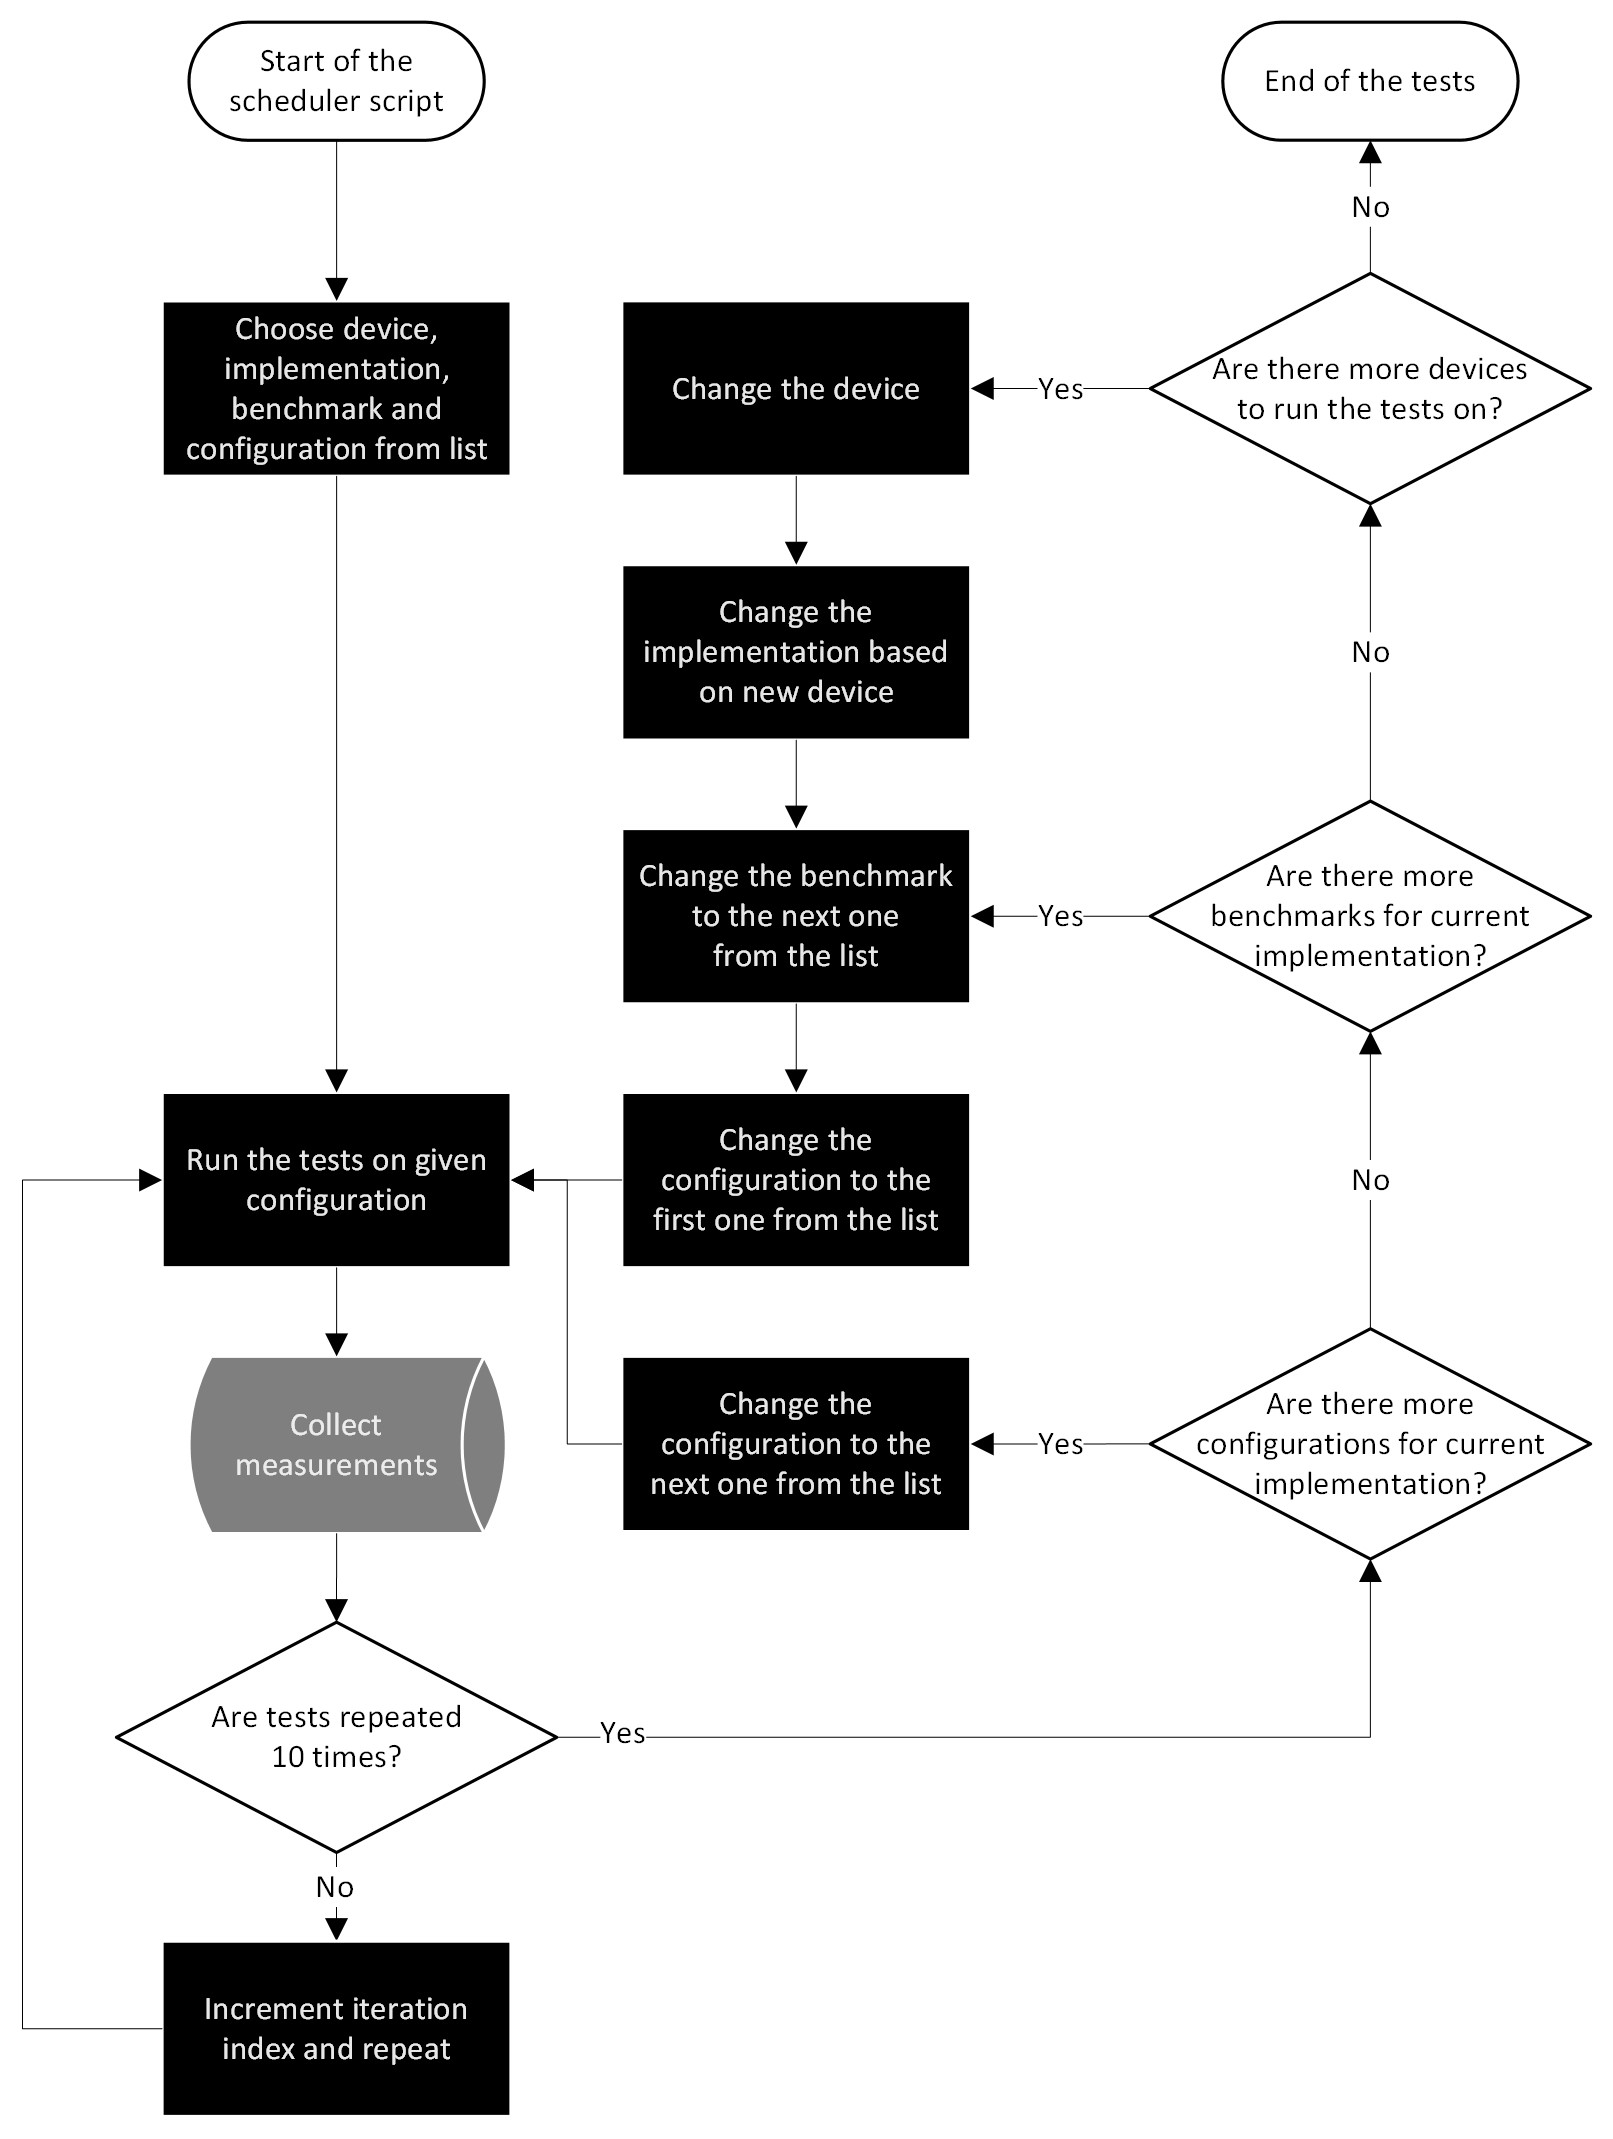
\includegraphics{general_flowchart}
    \caption{General Flowchart}~\label{fig:general_flowchart}
\end{figure}

\begin{figure}[hbtp!]
    \centering
    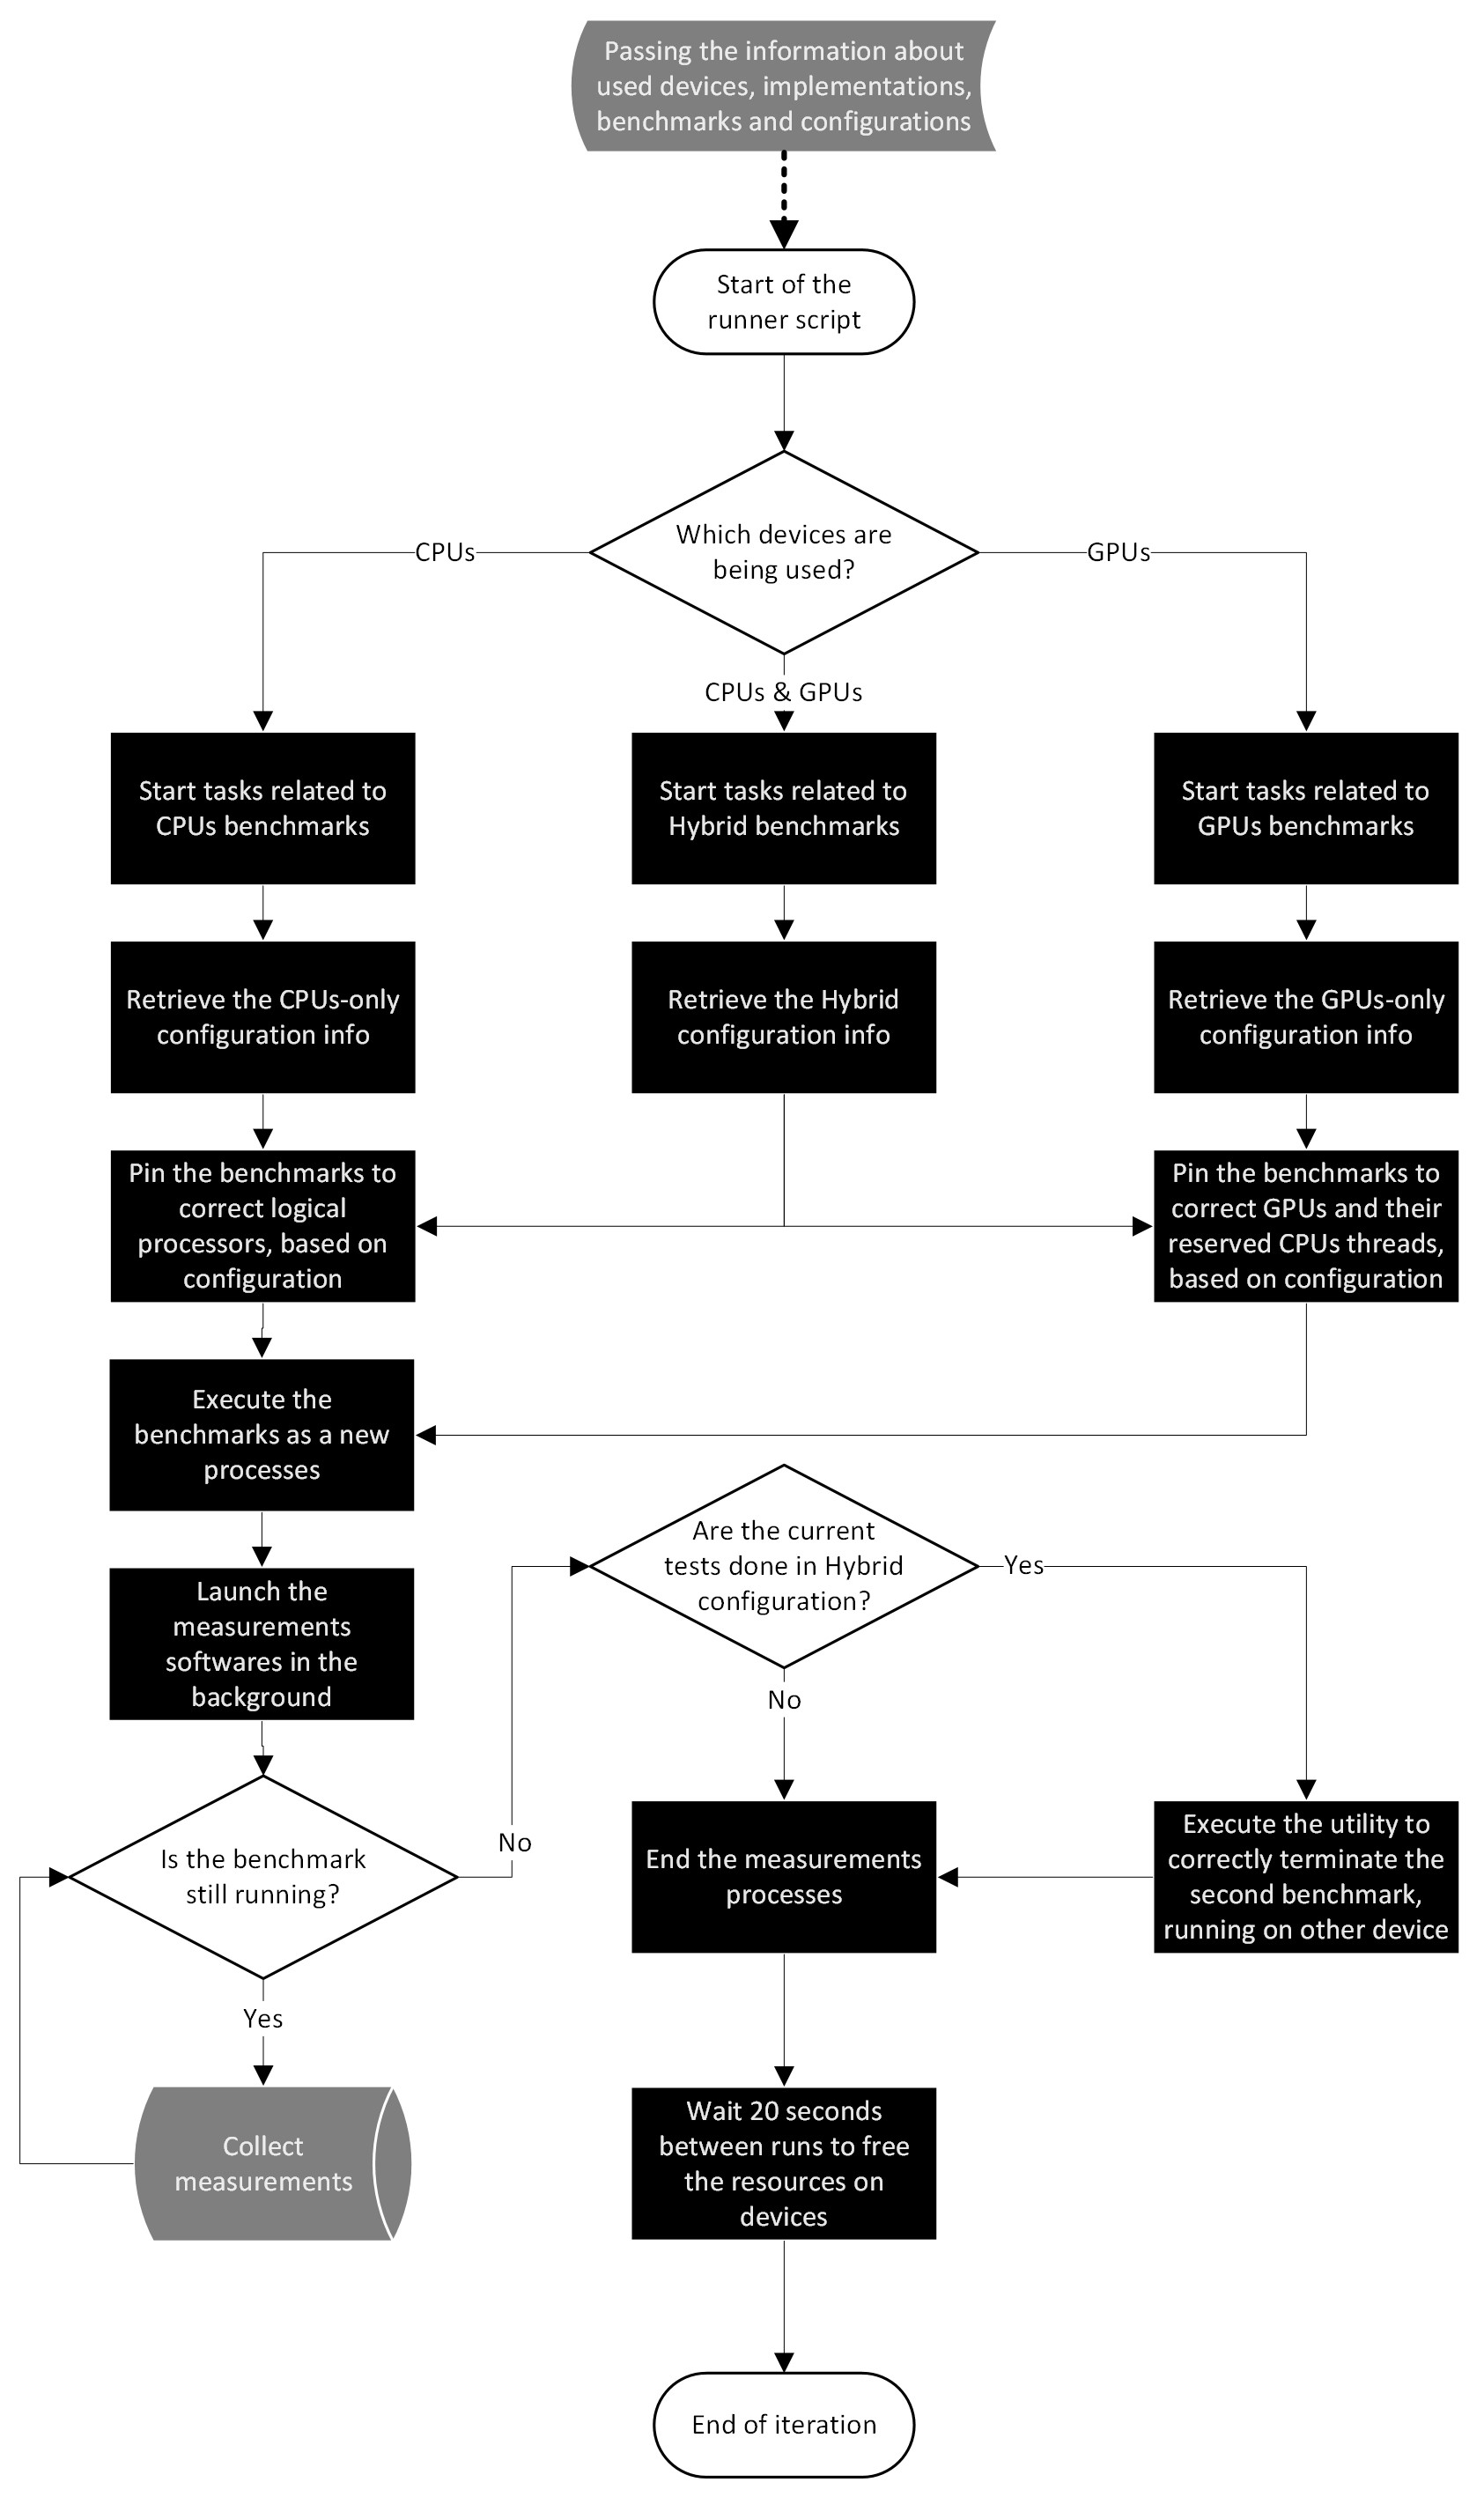
\includegraphics{processes_flowchart.jpeg}
    \caption{Processes Flowchart}~\label{fig:processes_flowchart}
\end{figure}

\newpage

% \subsection{Threads pinning and kernels execution $-$ cpu\_benchmark()}
\subsection{Threads pinning and kernels execution}

This function is responsible of executing CPUs benchmarks, based on the
given configuration. It creates a separate processes by utilizing the
Python \emph{subprocess} module. 

\begin{lstlisting}[language=Python]
    cpu_benchmark = subprocess.Popen(
        [
            "taskset --cpu-list <T> <P> <B> > /dev/null 2>&1"
        ],
        shell=True
    )
    return cpu_benchmark.pid
\end{lstlisting}

Here is an explanation of every part of the command:

\begin{itemize}
    \item \textbf{cpu\_benchmark} $-$ A variable of type
    \emph{<class `subprocess.Popen'>} is created mainly in order to
    retrieve PID later on.
    \item \textbf{subprocess.Popen} $-$ The underlying process creation and
    management is handled by the Popen class. Its function is to execute
    a child program in a new process.
    \item \textbf{taskset} $-$ This command is used to set or retrieve the
    CPU affinity of a running process given its pid, or to launch a new
    command with a given CPU affinity.
    \item \textbf{--cpu-list} $-$ This option interprets mask as numerical
    list of processors instead of a bitmask. Numbers are separated by
    commas and may include ranges. For example: 0,5,8-11.
    \item Variables that dynamically changes based on the configurations:
    \begin{conditions}
        \textbf{T} & Logical processors indexes \\
        \textbf{P} & Specified absolute path to the correct measurements folder \\
        \textbf{B} & Currently used benchmark kernel \\
    \end{conditions}
    \item \textbf{\textgreater~/dev/null 2\textgreater\&1} $-$
    Redirecting \emph{stderr} containing error messages from the
    executed command or script to \emph{stdout} to the output of the
    command. Both are, in fact, redirected then to the so-called
    \emph{null device}. The result of that action is suppression of all
    messages printed by the benchmark kernels. It is useful when
    collecting logs from the terminal, that is running the entire
    scheduler script, without unnecessary messages.
    \item \textbf{shell=True} $-$ Invokes the program as `shell'
\end{itemize}

Finally, the function returns the PID of newly created process
as an integer value. It is done for the purpose of terminating the
benchmark in a Hybrid configuration.

\newpage

% \subsection{GPUs and threads management $-$ gpu\_benchmark\@()}
\subsection{GPUs and threads management}

This function consists of two parts: first part is responsible for executing
the Horovod-Python benchmark and the second part is responsible for running
the OMP-CUDA benchmark.

\begin{lstlisting}[language=Python]
    gpu_benchmark = subprocess.Popen(
        [
            "mpirun -np <N> --map-by socket -x NCCL_DEBUG=INFO \
            python3 <P>+"Xception.py > /dev/null 2>&1"
        ],
        shell=True
    )
    return gpu_benchmark.pid
\end{lstlisting}

Here is an explanation of every part of the command:

\begin{itemize}
    \item \textbf{gpu\_benchmark} $-$ A variable of type
    \emph{<class `subprocess.Popen'>} is created mainly in order to
    retrieve PID later on.
    \item \textbf{subprocess.Popen} $-$ The underlying process creation and
    management is handled by the Popen class. Its function is to execute
    a child program in a new process.
    \item \textbf{mpirun} $-$ This command is used to execute serial and
    parallel jobs. It will run X copies of specified program in the current
    run-time environment and scheduling (by default) in a~round-robin fashion
    by CPU slot.
    \item \textbf{-np} $-$ This option specifies, how many processes will be
    started.
    \item Variables that dynamically changes based on the configurations:
    \begin{conditions}
        \textbf{N} & Number of GPUs used in training \\
        \textbf{P} & Specified absolute path to the correct measurements folder \\
    \end{conditions}
    \item \textbf{--map-by socket} $-$ Map to the specified object, such as 
    slot, hwthread, core, socket, numa, board, node and more. In this
    particular case, benchmark application is mapped by `socket', allowing to
    utilize multiple GPUs for training in a ditributed manner.
    \item \textbf{-x} $-$ Export the specified environment variables to the
    remote nodes before executing the program.
    \item \textbf{NCCL\_DEBUG=INFO} $-$ This flag is used for debugging. In
    case of NCCL failure, you can set NCCL\_DEBUG=INFO to print an explicit
    warning message as well as basic NCCL initialization information.
    \item \textbf{python3} $-$ Specify the use of Python interpreter when
    executing the script of deep neural networks model training.
    \item \textbf{Xception.py} $-$ Name of the script file.
    \item \textbf{\textgreater~/dev/null 2\textgreater\&1} $-$
    As mentioned in the previous subsection, this command suppresses the
    output from the terminal, in order to avoid the unnecessary messages.
    \item \textbf{shell=True} $-$ Invokes the program as `shell'
\end{itemize}

Finally, the function returns the PID of newly created process
as an integer value. It is done for the purpose of terminating the
benchmark in a Hybrid configuration.

\newpage

The second part of the function that runs the OMP-CUDA benchmarks is as
follows:

\begin{lstlisting}[language=Python]
    list_of_gpu_benchmarks = []
    value = Config.taskset_gpu[configuration_gpu]
    for i in range(0, len(value), 1):
        gpu_benchmark = subprocess.Popen(
            [
                "taskset --cpu-list <I> <P+I> <B> > /dev/null 2>&1"
            ],
            shell=True,
        )
        list_of_gpu_benchmarks.append(gpu_benchmark.pid)
    return list_of_gpu_benchmarks
\end{lstlisting}

Here is an explanation of every part of the command:

\begin{itemize}
    \item \textbf{gpu\_benchmark} $-$ A variable of type
    \emph{<class `subprocess.Popen'>} is created mainly in order to
    retrieve PID later on.
    \item \textbf{subprocess.Popen} $-$ The underlying process creation and
    management is handled by the Popen class. Its function is to execute
    a child program in a new process.
    \item \textbf{taskset} $-$ This command is used to set or retrieve the
    CPU affinity of a running process given its pid, or to launch a new
    command with a given CPU affinity.
    \item \textbf{--cpu-list} $-$ This option interprets mask as numerical
    list of processors instead of a bitmask. Numbers are separated by
    commas and may include ranges.
    \item Variables that dynamically changes based on the configurations:
    \begin{conditions}
        \textbf{I} & \parbox[t]{12cm}{Allocation of individual logical
        processors to the GPUs, based on the index number from special
        dictionary} \\
        \textbf{P+I} & \parbox[t]{12cm}{Specified absolute path to
        the correct measurements folder, modified by the number of total GPUs
        used} \\
        \textbf{B} & Currently used benchmark kernel \\
    \end{conditions}
    \item \textbf{\textgreater~/dev/null 2\textgreater\&1} $-$
    As mentioned in the previous subsection, this command suppresses the
    output from the terminal, in order to avoid the unnecessary messages.
    \item \textbf{shell=True} $-$ Invokes the program as `shell'
    \item \textbf{list\_of\_gpu\_benchmarks.append\@(gpu\_benchmark.pid)} $-$
    Filling the list with PIDs of benchmarks for later termination.
\end{itemize}

Finally, the function returns the PID of newly created process
as an integer value. In this particular case, if there are more than one GPUs
used in tests, the PIDs of all spawned processes are parsed as a list to the
function that is responsible in orderly terminating all the kernels.

\newpage

% \subsection{Measurements with Yokotool software $-$ yoko\@()}
\subsection{Measurements with Yokotool software}

This function utilizes the high-level Python wrapper for Yokogawa WT310E Power
Meter, the \emph{Yokotool}.

Syntax is similar to the previous examples:

\begin{lstlisting}[language=Python]
    yokotool = subprocess.Popen(
        [
            "yokotool read T,P -o <P+N> > /dev/null 2>&1 &"
        ],
        shell=True
    )
    return yokotool.pid
\end{lstlisting}

Here is an explanation of every part of the command:

\begin{itemize}
    \item \textbf{yokotool} $-$ Yokotool's command line interface is based
    on commands and sub-commands, similar to git and many other tools. This
    invokes the Yokotool wrapper for use.
    \item \textbf{read} $-$ Read measurements data.
    \item \textbf{T,P} $-$ Specifies, what data we want to read. In this
    particular case it is time \textbf{T} measured from the start of the epoch
    (on `UNIX time' is starts at 00:00:00 UTC on 1 January 1970) and power
    \textbf{P}, measured in Watts [W]. Output is separated with comma for
    easy manipulation of data after tests.
    \item \textbf{-o} $-$ This flags redirects the output from the
    measurements to a file for later analysis.
    \item Variables that dynamically changes based on the configurations:
    \begin{conditions}
        \textbf{P+N} & \parbox[t]{12cm}{Specified absolute path to
        the correct measurements folder, modified by the current number of
        iterations} \\
    \end{conditions}
    \item \textbf{\textgreater~/dev/null 2\textgreater\&1} $-$
    As mentioned in the previous subsection, this command suppresses the
    output from the terminal, in order to avoid the unnecessary messages.
    In this case, and additional \& is placed at the end, which means that
    the entire command is put as a~background process.
    \item \textbf{shell=True} $-$ Invokes the program as `shell'
\end{itemize}

Finally, the function returns the PID of newly created process
as an integer value. It is done for the purpose of terminating the
measurements by the designated function.

\newpage

% \subsection{Measurements with Linux Perf software $-$ perf\@()}
\subsection{Measurements with Linux Perf software}

Linux Perf is a lightweight profiling tool with performance counters.
It utilizes Intel RAPL for measurements of pre-defined events on CPUs.
To obtain more informations about what can be measured by Linux Perf,
one can use \emph{perf list} command in the terminal.

\begin{lstlisting}[language=Python]
    list_of_perf_pids = []
    pin_to_cpus = ("0", "10")
    idx_names = {"0": "0", "10": "1"}
    for i in pin_to_cpus:
        perf = subprocess.Popen(
            [
                "perf stat --event=power/energy-pkg/ \
                --cpu=<C> --delay 100 --interval-print 100 \
                --summary --field-separator , \
                --output <P+N> > /dev/null 2>&1 &"
            ],
            shell = True,
        )
        list_of_perf_pids.append(perf.pid)
    return list_of_perf_pids
\end{lstlisting}

Here is an explanation of every part of the command:

\begin{itemize}
    \item \textbf{perf} $-$ Invocation of measurements tool.
    \item \textbf{stat} $-$ Run a command and gather performance counter
    statistics.
    \item \textbf{--event=power/energy-pkg/} $-$ Event selector, in this case,
    the measured physical quantity is the energy usage of selected CPUs,
    during the benchmark kernel execution.
    \item \textbf{--cpu=<C>} $-$ Targeting of a specific CPU\. Correct integer
    value is based on the output of \emph{lscpu} command and the information
    about \emph{NUMA node\@(s)}.
    \item \textbf{--delay 100} $-$ A small delay of 100 [ms] is introduced in
    order to offset the slight delay of measurements of Yokogawa power meter.
    This solution has been introduced as a result of an observation during the
    preliminary tests. 
    \item \textbf{--interval-print 100} $-$ Measurements are performed with
    the same time interval of 100 [ms] set as two others measurements methods.
    \item \textbf{--summary} $-$ At the end of the measurements, an additional
    information about total energy used during tests, as well as the total
    measurements time is given. Mainly used during preliminary tests as an
    additional insight on gathered results.
    \item \textbf{--field-separator \,} $-$ Sets the output delimiter for
    easier access in softwares like LibreOffice $-$ every printed value is
    separated by commas `\,'
    \item \textbf{--output} $-$ Saves measurements to file. In this case,
    file names matches the consecutive runs.
    \item Variables that dynamically changes based on the configurations:
    \begin{conditions}
        \textbf{P+N} & \parbox[t]{12cm}{Specified absolute path to
        the correct measurements folder, modified by the current number of
        iterations} \\
    \end{conditions}
    \item \textbf{\textgreater~/dev/null 2\textgreater\&1} $-$
    Silences the output, redirecting it to null device and puts the process
    in the background.
    \item \textbf{shell=True} $-$ Invokes the program as `shell'
\end{itemize}

Finally, the function returns the PID of newly created process
as an integer value. It is done for the purpose of terminating the
measurements by the designated function.

% \subsection{Measurements with NVML handling function $-$ nvml\@()}
\subsection{Measurements with NVML handling function}

The method of gathering the measurements of power draw of GPUs, using NVIDIA
Management Library is a little different than in previously shown
implementations. No new processes are spawned, due to the fact, that the
measurements are handled by a special function already implemented in the
scheduler script. This function has two core parts: the first one is
responsible of precise executing the measurements every 100 [ms] $-$ it works
as an built-in scheduler, and the second part handled the invocation of
NVML-specific functions and saving the results to the file.

A short code-snippet below illustrates the practical usage of NVML related
function

\begin{lstlisting}[language=Python]
    import py3nvml
    nvmlInit()
    handle_Idx0 = nvmlDeviceGetHandleByIndex(0)
    # based on number of GPUs used, there are more
    # variables of that kind
    measure_Idx0 = nvmlDeviceGetPowerUsage(handle_Idx0) / 1000.0
    # rest of code contains the sub-scheduler routine
    # and saves the output to file.
\end{lstlisting}

\begin{itemize}
    \item \textbf{import py3nvml} $-$ Import of a module, that function as
    a high level Python wrapper for NVML\@.
    \item \textbf{nvmlInit\@()} $-$ NVIDIA Management Library initialization.
    It is mandatory to run before calling any other methods.
    \item \textbf{handle\_Idx0 = nvmlDeviceGetHandleByIndex\@(0)} $-$ create
    variable \emph{handle\_Idx0} and assign the return value of data type
    \emph{<class `py3nvml.py3nvml.LP\_struct\_c\_nvmlDevice\_t'>}, which is,
    in fact, a pointer to a memory register containing data about specific
    GPU\@.
    \item \textbf{measure\_Idx0 = nvmlDeviceGetPowerUsage\@(handle\_Idx0) / 1000.0}
    $-$ This function return a value of power draw of a specified GPU, in
    Watts [W]. 
\end{itemize}

In terms of proper ending the measurements process, this task is handled quite
differently than in previous implementations. The \emph{nvml\@()} function is
started as a parallel thread, using \emph{multiprocessing.Process\@()} module.
The thread is then started as a daemon, collecting measurements and saving
them in the background. After the end of benchmark kernel, the function is
ended by using innate multiprocessing function $-$ \emph{.terminate\@()}.

\newpage

\subsection{Termination of benchmarks in Hybrid configuration}

In order to make sure that the Hybrid benchmarks starts and ends at the same
time, an additional subroutine has been implemented. At first, the condition
is checked if used \emph{devices} in tests are currently set to \emph{Hybrid}.
Then, a special `while' loop is started, in which a special functions checks,
if CPUs and GPUs benchmarks are still running. They work by periodically
checking, if PID associated with respective kernels still exists. If the 
benchmark on one of the devices has ended, then the second one should be
terminated as well. The flag is passed to a function that, based on PID or
PIDs of the second benchmark, starts the cleaning process. Major facilitation
comes from the utilities of \emph{psutil} module. This solution allows to
easily find all the child processes spawned by the parent benchmark process,
terminate them iteratively in a ordered manner, and finally, terminate the
parent process. After that, the measurements threads are terminated via
another, designated for that function and the current run is ended.

\subsection{Cleanup of measurements daemons}

In terms of the termination of measurements daemons, a single function
handles Linux Perf, NVIDIA Management Library and Yokotool. It utilizes two
popular Python modules: \emph{os} and \emph{signal}. The first module provides
a portable way of using operating system dependent
functionality~\cite{Python_os_module}, while the second allows defining custom
handlers to be executed when a signal is received~\cite{Python_signal_module}.
In case of Perf and Yokotool, at first, the PIDs of those processes are being
received, either by using \emph{pidof} or \emph{pigrep} of those daemons.
Then, they are terminated using following, quite self-explanatory command:

\begin{lstlisting}[language=Python]
    os.kill(<PID>, signal.SIGTERM)
\end{lstlisting}

Since measurements of GPUs power draw that uses NVML are incorporated directly
into the scheduler script as an function, the entire thread is being handled
and terminated by using the function, that comes from \emph{multiprocessing}
module $-$ \emph{.terminate\@()}.

\section{Analysis of the results and discussion}

This section contains a summary of tables with measurements results as well as
the analysis of the dependencies between individual results.

The first set of tables contains the information about the average power draw
and average energy used for every configuration chosen during the preliminary
tests. The tables themselves are self-explanatory, the captions associated
with them gives hints about used server, device, implementation, benchmark
and finally, the data displayed. 

Two things should be noted, however. First, the physical quantities with label
(Yokogawa) means that the measurements has been done using Yokogawa WT310E
Power Meter and are related to the entire node, while those with labels
(CPU\@: <index>) and (GPU\@: <index>) are related to measurements done using
Linux Perf and NVML respectively. Second, the configurations execution
times vary $-$ majority of the tests have shorter execution times the more
resources of used devices are dedicated. Such configurations are\@:
OMP-CPP benchmarks for \emph{sanna.kask}, MPI-Fortran and Horovod-Python
for \emph{vinnana.kask} and their hybrid variants. This is due to the fact,
those implementations utilize parallel programmings paradigms, therefore the
execution speed-up can be observed. In case of the OMP-CUDA benchmarks,
situation is different $-$ those benchmarks were prepared for single GPU tests
only. Since the main purpose of the benchmarks is to simply strain and fully
utilize the devices resources, rather than compute meaningful research
problems, the OMP-CUDA benchmarks on multi-GPUs are simply many instances of
the same benchmark, running on different GPUs. Since those kernels are
independent from each other, the average execution times between configurations
are rougly the same. This also explains the fact, that the Hybrid benchmarks
that were run on \emph{sanna.kask} has sometimes shorter execution times the
more resources are dedicated and sometimes and sometimes they are similar.
The Hybrid benchmarks works in a way, that the listener function from the
scheduler script checks, whether the benchmarks are running or not. If the
CPUs benchmarks ends, the termination signal is send to GPUs benchmarks,
resulting with varying execution times. If the GPUs benchmarks in given
configuration ends faster, the CPUs benchmarks are terminated in return,
resulting in similar execution times.



\newpage

\begin{table}[hbt!]
    \rowcolors{1}{Lavender!80!gray}{white}
    \centering
    \caption{server: \textbf{sanna.kask}, device: \textbf{1 CPU}, implementation: \textbf{OMP-CPP},\\
    benchmark: \textbf{bt.C}, data displayed: \textbf{power draw}}\label{tbl:OMP-CPP_1CPU_btC_power}
    \setlength{\tabcolsep}{5mm}
    \begin{tblr}{
        vlines,
        row{1}={font=\bfseries,halign=c,bg=lightgray!30},
        row{2,5-6,9-10,13-14,17-18,21-22,25-26} = {bg = lightgray!30}
        }
    \hline
        & \SetCell[c=4]{c} 1 CPU  \\
    \hline
        Results from 10 runs                                    & 1 Thread  & 5 Threads & 10 Threads    & 20 Threads \\
    \hline
        {Avg. Exec\@. time [s]}                                 & 1054.795  & 216.315   & 114.315       & 101.372 \\
    \hline
        {Std\@. dev\@. of time [-]}                             & 0.966     & 0.243     & 0.121         & 0.158 \\
    \hline
        {(Yokogawa) \\ Avg\@. power draw [W]}                   & 379.962   & 402.881   & 432.171       & 445.752 \\
    \hline
        {(Yokogawa) \\ Std\@. dev\@. of avg\@. power draw [-]}  & 0.605     & 0.225     & 0.382         & 1.007 \\
    \hline
        {(CPU\@: 0) \\ Avg\@. power draw [W]}                   & 33.717    & 51.274    & 70.433        & 77.958 \\
    \hline
        {(CPU\@: 0) \\ Std\@. dev\@. of avg\@. power draw [-]}  & 0.102     & 0.13      & 0.085         & 0.089 \\
    \hline
        {(CPU\@: 1) \\ Avg\@. power draw [W]}                   & 28.98     & 28.887    & 28.871        & 28.874 \\
    \hline
        {(CPU\@: 1) \\ Std\@. dev\@. of avg\@. power draw [-]}  & 0.125     & 0.062     & 0.067         & 0.055 \\
    \hline
        {(GPU\@: 0) \\ Avg\@. power draw [W]}                   & 21.755    & 21.673    & 21.604        & 21.634 \\
    \hline
        {(GPU\@: 0) \\ Std\@. dev\@. of avg\@. power draw [-]}  & 0.343     & 0.061     & 0.2           & 0.05 \\
    \hline
        {(GPU\@: 1) \\ Avg\@. power draw [W]}                   & 25.522    & 25.534    & 25.516        & 25.524 \\
    \hline
        {(GPU\@: 1) \\ Std\@. dev\@. of avg\@. power draw [-]}  & 0.023     & 0.032     & 0.052         & 0.029 \\
    \hline
        {(GPU\@: 2) \\ Avg\@. power draw [W]}                   & 13.96     & 14.024    & 13.744        & 13.642 \\
    \hline
        {(GPU\@: 2) \\ Std\@. dev\@. of avg\@. power draw [-]}  & 0.117     & 0.114     & 0.243         & 0.157 \\
    \hline
        {(GPU\@: 3) \\ Avg\@. power draw [W]}                   & 17.196    & 17.21     & 17.207        & 17.209 \\
    \hline
        {(GPU\@: 3) \\ Std\@. dev\@. of avg\@. power draw [-]}  & 0.016     & 0.022     & 0.015         & 0.012 \\
    \hline
        {(GPU\@: 4) \\ Avg\@. power draw [W]}                   & 4.109     & 4.122     & 4.119         & 4.096 \\
    \hline
        {(GPU\@: 4) \\ Std\@. dev\@. of avg\@. power draw [-]}  & 0.01      & 0.018     & 0.016         & 0.012 \\
    \hline
        {(GPU\@: 5) \\ Avg\@. power draw [W]}                   & 18.456    & 18.372    & 18.297        & 18.334 \\
    \hline
        {(GPU\@: 5) \\ Std\@. dev\@. of avg\@. power draw [-]}  & 0.04      & 0.097     & 0.107         & 0.111 \\
    \hline
        {(GPU\@: 6) \\ Avg\@. power draw [W]}                   & 6.285     & 6.3       & 6.351         & 6.449 \\
    \hline
        {(GPU\@: 6) \\ Std\@. dev\@. of avg\@. power draw [-]}  & 0.075     & 0.08      & 0.146         & 0.075 \\
    \hline
        {(GPU\@: 7) \\ Avg\@. power draw [W]}                   & 12.174    & 12. 163   & 12.071        & 12.134 \\
    \hline
        {(GPU\@: 7) \\ Std\@. dev\@. of avg\@. power draw [-]}  & 0.313     & 0.14      & 0.316         & 0.311 \\
    \hline
    \end{tblr}
\end{table}

\begin{table}[hbt!]
    \rowcolors{1}{Lavender!80!gray}{white}
    \centering
    \caption{server: \textbf{sanna.kask}, device: \textbf{1 CPU}, implementation: \textbf{OMP-CPP},\\
    benchmark: \textbf{bt.C}, data displayed: \textbf{energy used}}\label{tbl:OMP-CPP_1CPU_btC_energy}
    \setlength{\tabcolsep}{5mm}
    \begin{tblr}{
        vlines,
        row{1}={font=\bfseries,halign=c,bg=lightgray!30},
        row{2,5-6,9-10,13-14,17-18,21-22,25-26} = {bg = lightgray!30}
        }
    \hline
        & \SetCell[c=4]{c} 1 CPU  \\
    \hline
        Results from 10 runs                                        & 2 Threads & 10 Threads    & 20 Threads    & 40 Threads \\
    \hline
        {Avg. Exec\@. time [s]}                                     & 1054.795  & 216.315   & 114.315       & 101.372 \\
    \hline
        {Std\@. dev\@. of time [-]}                                 & 0.966     & 0.243     & 0.121         & 0.158 \\
    \hline
        {(Yokogawa) \\ Avg\@. energy used [kJ]}                     & 4006.66   & 870.223   & 492.718       & 450.299 \\
    \hline
        {(Yokogawa) \\ Std\@. dev\@. of avg\@. energy used [-]}     & 7.695     & 1.038     & 0.644         & 1.35 \\
    \hline
        {(CPU\@: 0) \\ Avg\@. energy used [kJ]}                     & 35.555    & 11.078    & 8.033         & 7.883 \\
    \hline
        {(CPU\@: 0) \\ Std\@. dev\@. of avg\@. energy used [-]}     & 0.123     & 0.032     & 0.012         & 0.006 \\
    \hline
        {(CPU\@: 1) \\ Avg\@. energy used [kJ]}                     & 30.56     & 6.241     & 3.293         & 2.92 \\
    \hline
        {(CPU\@: 1) \\ Std\@. dev\@. of avg\@. energy used [-]}     & 0.145     & 0.015     & 0.009         & 0.006 \\
    \hline
        {(GPU\@: 0) \\ Avg\@. energy used [kJ]}                     & 229.411   & 46.824    & 24.642        & 21.805 \\
    \hline
        {(GPU\@: 0) \\ Std\@. dev\@. of avg\@. energy used [-]}     & 3.68      & 0.131     & 0.224         & 0.051 \\
    \hline
        {(GPU\@: 1) \\ Avg\@. energy used [kJ]}                     & 269.144   & 55.166    & 29.104        & 25.81 \\
    \hline
        {(GPU\@: 1) \\ Std\@. dev\@. of avg\@. energy used [-]}     & 0.244     & 0.1       & 0.062         & 0.039 \\
    \hline
        {(GPU\@: 2) \\ Avg\@. energy used [kJ]}                     & 147.218   & 30.298    & 15.676        & 13.795 \\
    \hline
        {(GPU\@: 2) \\ Std\@. dev\@. of avg\@. energy used [-]}     & 1.259     & 0.253     & 0.278         & 0.16 \\
    \hline
        {(GPU\@: 3) \\ Avg\@. energy used [kJ]}                     & 181.342   & 37.183    & 19.626        & 17.402 \\
    \hline
        {(GPU\@: 3) \\ Std\@. dev\@. of avg\@. energy used [-]}     & 0.229     & 0.061     & 0.024         & 0.024 \\
    \hline
        {(GPU\@: 4) \\ Avg\@. energy used [kJ]}                     & 43.328    & 8.905     & 4.698         & 4.142 \\
    \hline
        {(GPU\@: 4) \\ Std\@. dev\@. of avg\@. energy used [-]}     & 0.113     & 0.044     & 0.016         & 0.014 \\
    \hline
        {(GPU\@: 5) \\ Avg\@. energy used [kJ]}                     & 194.623   & 39.693    & 20.87         & 18.539 \\
    \hline
        {(GPU\@: 5) \\ Std\@. dev\@. of avg\@. energy used [-]}     & 0.432     & 0.212     & 0.13          & 0.112 \\
    \hline
        {(GPU\@: 6) \\ Avg\@. energy used [kJ]}                     & 66.28     & 13.611    & 7.244         & 6.522 \\
    \hline
        {(GPU\@: 6) \\ Std\@. dev\@. of avg\@. energy used [-]}     & 0.781     & 0.167     & 0.168         & 0.078 \\
    \hline
        {(GPU\@: 7) \\ Avg\@. energy used [kJ]}                     & 128.383   & 26.278    & 13.769        & 12.27 \\
    \hline
        {(GPU\@: 7) \\ Std\@. dev\@. of avg\@. energy used [-]}     & 3.336     & 0.312     & 0.358         & 0.318 \\
    \hline
    \end{tblr}
\end{table}

\begin{table}[hbt!]
    \rowcolors{1}{Lavender!80!gray}{white}
    \centering
    \caption{server: \textbf{sanna.kask}, device: \textbf{2 CPUs}, implementation: \textbf{OMP-CPP},\\
    benchmark: \textbf{bt.C}, data displayed: \textbf{power draw}}\label{tbl:OMP-CPP_2CPUs_btC_power}
    \setlength{\tabcolsep}{5mm}
    \begin{tblr}{
        vlines,
        row{1}={font=\bfseries,halign=c,bg=lightgray!30},
        row{2,5-6,9-10,13-14,17-18,21-22,25-26} = {bg = lightgray!30}
        }
    \hline
        & \SetCell[c=4]{c} 2 CPUs  \\
    \hline
        Results from 10 runs                                    & 2 Threads & 10 Threads    & 20 Threads    & 40 Threads \\
    \hline
        {Avg. Exec\@. time [s]}                                 & 861.634   & 114.56        & 69.86         & 64.855 \\
    \hline
        {Std\@. dev\@. of time [-]}    [FIX THIS RUN!!!]        & 107.726   & 1.843         & 0.395         & 0.979 \\
    \hline
        {(Yokogawa) \\ Avg\@. power draw [W]}                   & 382.827   & 432.746       & 477.802       & 500.032 \\
    \hline
        {(Yokogawa) \\ Std\@. dev\@. of avg\@. power draw [-]}  & 1.469     & 0.575         & 1.18          & 2.708 \\
    \hline
        {(CPU\@: 0) \\ Avg\@. power draw [W]}                   & 33.397    & 51.044        & 65.793        & 71.718 \\
    \hline
        {(CPU\@: 0) \\ Std\@. dev\@. of avg\@. power draw [-]}  & 0.336     & 0.188         & 0.175         & 0.372 \\
    \hline
        {(CPU\@: 1) \\ Avg\@. power draw [W]}                   & 31.426    & 49.813        & 65.932        & 71.781 \\
    \hline
        {(CPU\@: 1) \\ Std\@. dev\@. of avg\@. power draw [-]}  & 1.188     & 0.239         & 0.166         & 0.358 \\
    \hline
        {(GPU\@: 0) \\ Avg\@. power draw [W]}                   & 21.634    & 21.663        & 21.595        & 21.714 \\
    \hline
        {(GPU\@: 0) \\ Std\@. dev\@. of avg\@. power draw [-]}  & 0.105     & 0.115         & 0.064         & 0.068 \\
    \hline
        {(GPU\@: 1) \\ Avg\@. power draw [W]}                   & 25.556    & 25.553        & 25.577        & 25.549 \\
    \hline
        {(GPU\@: 1) \\ Std\@. dev\@. of avg\@. power draw [-]}  & 0.039     & 0.029         & 0.047         & 0.025 \\
    \hline
        {(GPU\@: 2) \\ Avg\@. power draw [W]}                   & 14.01     & 13.63         & 13.701        & 13.732 \\
    \hline
        {(GPU\@: 2) \\ Std\@. dev\@. of avg\@. power draw [-]}  & 0.172     & 0.153         & 0.134         & 0.132 \\
    \hline
        {(GPU\@: 3) \\ Avg\@. power draw [W]}                   & 17.213    & 17.181        & 17.207        & 17.204 \\
    \hline
        {(GPU\@: 3) \\ Std\@. dev\@. of avg\@. power draw [-]}  & 0.012     & 0.012         & 0.021         & 0.022 \\
    \hline
        {(GPU\@: 4) \\ Avg\@. power draw [W]}                   & 4.091     & 4.11          & 4.108         & 4.105 \\
    \hline
        {(GPU\@: 4) \\ Std\@. dev\@. of avg\@. power draw [-]}  & 0.006     & 0.025         & 0.01          & 0.017 \\
    \hline
        {(GPU\@: 5) \\ Avg\@. power draw [W]}                   & 18.414    & 18.358        & 18.574        & 18.639 \\
    \hline
        {(GPU\@: 5) \\ Std\@. dev\@. of avg\@. power draw [-]}  & 0.058     & 0.062         & 0.127         & 0.089 \\
    \hline
        {(GPU\@: 6) \\ Avg\@. power draw [W]}                   & 6.437     & 6.457         & 6.484         & 6.507 \\
    \hline
        {(GPU\@: 6) \\ Std\@. dev\@. of avg\@. power draw [-]}  & 0.189     & 0.11          & 0.103         & 0.17 \\
    \hline
        {(GPU\@: 7) \\ Avg\@. power draw [W]}                   & 12.281    & 12.136        & 11.891        & 11.98 \\
    \hline
        {(GPU\@: 7) \\ Std\@. dev\@. of avg\@. power draw [-]}  & 0.362     & 0.253         & 0.158         & 0.135 \\
    \hline
    \end{tblr}
\end{table}

\begin{table}[!htbp]
    \rowcolors{1}{Lavender!80!gray}{white}
    \centering
    \caption{server: \textbf{sanna.kask}, device: \textbf{2 CPUs}, implementation: \textbf{OMP-CPP},\\
    benchmark: \textbf{bt.C}, data displayed: \textbf{energy used}}\label{tbl:OMP-CPP_2CPUs_btC_energy}
    \setlength{\tabcolsep}{5mm}
    \begin{tblr}{
        vlines,
        row{1}={font=\bfseries,halign=c,bg=lightgray!30},
        row{2,5-6,9-10,13-14,17-18,21-22,25-26} = {bg = lightgray!30}
        }
    \hline
        & \SetCell[c=4]{c} 2 CPUs  \\
    \hline
        Results from 10 runs                                        & 2 Threads & 10 Threads    & 20 Threads    & 40 Threads \\
    \hline
        {Avg. Exec\@. time [s]}                                     & 955.334   & 114.56        & 69.86         & 64.855 \\
    \hline
        {Std\@. dev\@. of time [-]}                                 & 1.891     & 1.843         & 0.395         & 0.979 \\
    \hline
        {(Yokogawa) \\ Avg\@. energy used [kJ]}                     & 365.73    & 49.575        & 33.379        & 32.428 \\
    \hline
        {(Yokogawa) \\ Std\@. dev\@. of avg\@. energy used [-]}     & 1.935     & 0.739         & 0.188         & 0.39 \\
    \hline
        {(CPU\@: 0) \\ Avg\@. energy used [kJ]}                     & 28.779    & 5.834         & 4.578         & 4.63 \\
    \hline
        {(CPU\@: 0) \\ Std\@. dev\@. of avg\@. energy used [-]}     & 3.718     & 0.084         & 0.018         & 0.05 \\
    \hline
        {(CPU\@: 1) \\ Avg\@. energy used [kJ]}                     & 26.958    & 5.693         & 4.587         & 4.634 \\
    \hline
        {(CPU\@: 1) \\ Std\@. dev\@. of avg\@. energy used [-]}     & 2.456     & 0.07          & 0.024         & 0.05 \\
    \hline
        {(GPU\@: 0) \\ Avg\@. energy used [kJ]}                     & 20.668    & 2.482         & 1.509         & 1.408 \\
    \hline
        {(GPU\@: 0) \\ Std\@. dev\@. of avg\@. energy used [-]}     & 0.108     & 0.05          & 0.007         & 0.022 \\
    \hline
        {(GPU\@: 1) \\ Avg\@. energy used [kJ]}                     & 24.415    & 2.927         & 1.787         & 1.657 \\
    \hline
        {(GPU\@: 1) \\ Std\@. dev\@. of avg\@. energy used [-]}     & 0.055     & 0.046         & 0.011         & 0.024 \\
    \hline
        {(GPU\@: 2) \\ Avg\@. energy used [kJ]}                     & 13.384    & 1.562         & 0.957         & 0.891 \\
    \hline
        {(GPU\@: 2) \\ Std\@. dev\@. of avg\@. energy used [-]}     & 0.163     & 0.034         & 0.012         & 0.016 \\
    \hline
        {(GPU\@: 3) \\ Avg\@. energy used [kJ]}                     & 16.444    & 1.968         & 1.202         & 1.116 \\
    \hline
        {(GPU\@: 3) \\ Std\@. dev\@. of avg\@. energy used [-]}     & 0.032     & 0.031         & 0.006         & 0.017 \\
    \hline
        {(GPU\@: 4) \\ Avg\@. energy used [kJ]}                     & 3.908     & 0.471         & 0.287         & 0.266 \\
    \hline
        {(GPU\@: 4) \\ Std\@. dev\@. of avg\@. energy used [-]}     & 0.006     & 0.006         & 0.002         & 0.004 \\
    \hline
        {(GPU\@: 5) \\ Avg\@. energy used [kJ]}                     & 17.591    & 2.103         & 1.298         & 1.209 \\
    \hline
        {(GPU\@: 5) \\ Std\@. dev\@. of avg\@. energy used [-]}     & 0.064     & 0.036         & 0.007         & 0.021 \\
    \hline
        {(GPU\@: 6) \\ Avg\@. energy used [kJ]}                     & 6.149     & 0.74          & 0.453         & 0.422 \\
    \hline
        {(GPU\@: 6) \\ Std\@. dev\@. of avg\@. energy used [-]}     & 0.179     & 0.018         & 0.007         & 0.008 \\
    \hline
        {(GPU\@: 7) \\ Avg\@. energy used [kJ]}                     & 11.733    & 1.39          & 0.831         & 0.777 \\
    \hline
        {(GPU\@: 7) \\ Std\@. dev\@. of avg\@. energy used [-]}     & 0.351     & 0.028         & 0.011         & 0.014 \\
    \hline
    \end{tblr}
\end{table}



\begin{table}[hbt!]
    \rowcolors{1}{Lavender!80!gray}{white}
    \centering
    \caption{server: \textbf{sanna.kask}, device: \textbf{1 CPU}, implementation: \textbf{OMP-CPP},\\
    benchmark: \textbf{is.D}, data displayed: \textbf{power draw}}\label{tbl:OMP-CPP_1CPU_isD_power}
    \setlength{\tabcolsep}{5mm}
    \begin{tblr}{
        vlines,
        row{1}={font=\bfseries,halign=c,bg=lightgray!30},
        row{2,5-6,9-10,13-14,17-18,21-22,25-26} = {bg = lightgray!30}
        }
    \hline
        & \SetCell[c=4]{c} 1 CPU  \\
    \hline
        Results from 10 runs                                    & 1 Thread  & 5 Threads     & 10 Threads    & 20 Threads \\
    \hline
        {Avg. Exec\@. time [s]}                                 & 649       & 183.121       & 76.25         & 57.389 \\
    \hline
        {Std\@. dev\@. of time [-]}                             & 0.277     & 125.881 [FIX] & 0.26          & 0.056 \\
    \hline
        {(Yokogawa) \\ Avg\@. power draw [W]}                   & 378.666   & 394.555       & 413.561       & 426.861 \\
    \hline
        {(Yokogawa) \\ Std\@. dev\@. of avg\@. power draw [-]}  & 0.076     & 0.278         & 0.28          & 0.464 \\
    \hline
        {(CPU\@: 0) \\ Avg\@. power draw [W]}                   & 32.558    & 42.525        & 56.774        & 63.154 \\
    \hline
        {(CPU\@: 0) \\ Std\@. dev\@. of avg\@. power draw [-]}  & 0.032     & 5.14          & 0.01          & 0.048 \\
    \hline
        {(CPU\@: 1) \\ Avg\@. power draw [W]}                   & 28.52     & 28.607        & 29.026        & 29.05 \\
    \hline
        {(CPU\@: 1) \\ Std\@. dev\@. of avg\@. power draw [-]}  & 0.135     & 1.489         & 0.077         & 0.062 \\
    \hline
        {(GPU\@: 0) \\ Avg\@. power draw [W]}                   & 21.648    & 21.72         & 21.707        & 21.791 \\
    \hline
        {(GPU\@: 0) \\ Std\@. dev\@. of avg\@. power draw [-]}  & 0.056     & 0.063         & 0.04          & 0.076 \\
    \hline
        {(GPU\@: 1) \\ Avg\@. power draw [W]}                   & 25.545    & 25.563        & 25.548        & 25.504 \\
    \hline
        {(GPU\@: 1) \\ Std\@. dev\@. of avg\@. power draw [-]}  & 0.024     & 0.028         & 0.046         & 0.026 \\
    \hline
        {(GPU\@: 2) \\ Avg\@. power draw [W]}                   & 13.861    & 13.718        & 13.501        & 13.791 \\
    \hline
        {(GPU\@: 2) \\ Std\@. dev\@. of avg\@. power draw [-]}  & 0.161     & 0.142         & 0.148         & 0.166 \\
    \hline
        {(GPU\@: 3) \\ Avg\@. power draw [W]}                   & 17.227    & 17.235        & 17.209        & 17.225 \\
    \hline
        {(GPU\@: 3) \\ Std\@. dev\@. of avg\@. power draw [-]}  & 0.022     & 0.023         & 0.013         & 0.017 \\
    \hline
        {(GPU\@: 4) \\ Avg\@. power draw [W]}                   & 4.104     & 4.112         & 4.103         & 4.084 \\
    \hline
        {(GPU\@: 4) \\ Std\@. dev\@. of avg\@. power draw [-]}  & 0.016     & 0.013         & 0.017         & 0.02 \\
    \hline
        {(GPU\@: 5) \\ Avg\@. power draw [W]}                   & 18.345    & 18.483        & 18.409        & 18.436 \\
    \hline
        {(GPU\@: 5) \\ Std\@. dev\@. of avg\@. power draw [-]}  & 0.068     & 0.103         & 0.088         & 0.131 \\
    \hline
        {(GPU\@: 6) \\ Avg\@. power draw [W]}                   & 6.488     & 6.221         & 6.268         & 6.298 \\
    \hline
        {(GPU\@: 6) \\ Std\@. dev\@. of avg\@. power draw [-]}  & 0.157     & 0.074         & 0.095         & 0.116 \\
    \hline
        {(GPU\@: 7) \\ Avg\@. power draw [W]}                   & 12.351    & 12.097        & 12.134        & 12.576 \\
    \hline
        {(GPU\@: 7) \\ Std\@. dev\@. of avg\@. power draw [-]}  & 0.119     & 0.098         & 0.175         & 0.138 \\
    \hline
    \end{tblr}
\end{table}

\begin{table}[hbt!]
    \rowcolors{1}{Lavender!80!gray}{white}
    \centering
    \caption{server: \textbf{sanna.kask}, device: \textbf{1 CPU}, implementation: \textbf{OMP-CPP},\\
    benchmark: \textbf{is.D}, data displayed: \textbf{energy used}}\label{tbl:OMP-CPP_1CPU_isD_energy}
    \setlength{\tabcolsep}{5mm}
    \begin{tblr}{
        vlines,
        row{1}={font=\bfseries,halign=c,bg=lightgray!30},
        row{2,5-6,9-10,13-14,17-18,21-22,25-26} = {bg = lightgray!30}
        }
    \hline
        & \SetCell[c=4]{c} 1 CPU  \\
    \hline
        Results from 10 runs                                        & 1 Thread  & 5 Threads     & 10 Threads    & 20 Threads \\
    \hline
        {Avg. Exec\@. time [s]}                                     & 649       & 183.121       & 76.25         & 57.389 \\
    \hline
        {Std\@. dev\@. of time [-]}                                 & 0.277     & 125.881       & 0.26          & 0.056 \\
    \hline
        {(Yokogawa) \\ Avg\@. energy used [kJ]}                     & 245,754  & 56,548       & 31,534       & 24,497 \\
    \hline
        {(Yokogawa) \\ Std\@. dev\@. of avg\@. energy used [-]}     & 0,101     & 0,03        & 0,09         & 0,024 \\
    \hline
        {(CPU\@: 0) \\ Avg\@. energy used [kJ]}                     & 21.122    & 7.194         & 4.314         & 3.607 \\
    \hline
        {(CPU\@: 0) \\ Std\@. dev\@. of avg\@. energy used [-]}     & 0.028     & 2.777         & 0.014         & 0.004 \\
    \hline
        {(CPU\@: 1) \\ Avg\@. energy used [kJ]}                     & 18.502    & 5.063         & 2.206         & 1.659 \\
    \hline
        {(CPU\@: 1) \\ Std\@. dev\@. of avg\@. energy used [-]}     & 0.085     & 2.857         & 0.005         & 0.004 \\
    \hline
        {(GPU\@: 0) \\ Avg\@. energy used [kJ]}                     & 14,05   & 3,113        & 1,655       & 1,251 \\
    \hline
        {(GPU\@: 0) \\ Std\@. dev\@. of avg\@. energy used [-]}     & 0,034     & 0,009          & 0,008          & 0,004 \\
    \hline
        {(GPU\@: 1) \\ Avg\@. energy used [kJ]}                     & 16,579   & 3,664        & 1,948        & 1,464 \\
    \hline
        {(GPU\@: 1) \\ Std\@. dev\@. of avg\@. energy used [-]}     & 0,014     & 0,004         & 0,007         & 0,001 \\
    \hline
        {(GPU\@: 2) \\ Avg\@. energy used [kJ]}                     & 8,996     & 1,966        & 1,03        & 0,792 \\
    \hline
        {(GPU\@: 2) \\ Std\@. dev\@. of avg\@. energy used [-]}     & 0,103     & 0,021         & 0,013         & 0,009 \\
    \hline
        {(GPU\@: 3) \\ Avg\@. energy used [kJ]}                     & 11,18   & 2,47        & 1,312       & 0,988 \\
    \hline
        {(GPU\@: 3) \\ Std\@. dev\@. of avg\@. energy used [-]}     & 0,016     & 0,004         & 0,004         & 0,001 \\
    \hline
        {(GPU\@: 4) \\ Avg\@. energy used [kJ]}                     & 2,663    & 0,589         & 0,313         & 0,234 \\
    \hline
        {(GPU\@: 4) \\ Std\@. dev\@. of avg\@. energy used [-]}     & 0,01     & 0,002         & 0,002         & 0,001 \\
    \hline
        {(GPU\@: 5) \\ Avg\@. energy used [kJ]}                     & 11,906   & 2,649        & 1,403        & 1,058 \\
    \hline
        {(GPU\@: 5) \\ Std\@. dev\@. of avg\@. energy used [-]}     & 0,04       & 0,015         & 0,008         & 0,008 \\
    \hline
        {(GPU\@: 6) \\ Avg\@. energy used [kJ]}                     & 4,211    & 0,892         & 0,478         & 0,362 \\
    \hline
        {(GPU\@: 6) \\ Std\@. dev\@. of avg\@. energy used [-]}     & 0,103     & 0,011         & 0,007         & 0,007 \\
    \hline
        {(GPU\@: 7) \\ Avg\@. energy used [kJ]}                     & 8,016    & 1,734         & 0,925          & 0,722 \\
    \hline
        {(GPU\@: 7) \\ Std\@. dev\@. of avg\@. energy used [-]}     & 0,078     & 0,014         & 0,014         & 0,008 \\
    \hline
    \end{tblr}
\end{table}

\begin{table}[!htbp]
    \rowcolors{1}{Lavender!80!gray}{white}
    \centering
    \caption{server: \textbf{sanna.kask}, device: \textbf{2 CPUs}, implementation: \textbf{OMP-CPP},\\
    benchmark: \textbf{is.D}, data displayed: \textbf{power draw}}\label{tbl:OMP-CPP_2CPUs_btC_power}
    \setlength{\tabcolsep}{5mm}
    \begin{tblr}{
        vlines,
        row{1}={font=\bfseries,halign=c,bg=lightgray!30},
        row{2,5-6,9-10,13-14,17-18,21-22,25-26} = {bg = lightgray!30}
        }
    \hline
        & \SetCell[c=4]{c} 2 CPUs  \\
    \hline
        Results from 10 runs                                    & 2 Threads & 10 Threads    & 20 Threads    & 40 Threads \\
    \hline
        {Avg. Exec\@. time [s]}                                 & 393.075   & 86.848        & 47.879        & 38.223 \\
    \hline
        {Std\@. dev\@. of time [-]}                             & 7.964     & 2.783         & 1.263         & 1.377 \\
    \hline
        {(Yokogawa) \\ Avg\@. power draw [W]}                   & 383.887   & 414.22        & 447.238       & 470.243 \\
    \hline
        {(Yokogawa) \\ Std\@. dev\@. of avg\@. power draw [-]}  & 0.326     & 0.689         & 1.146         & 2.189 \\
    \hline
        {(CPU\@: 0) \\ Avg\@. power draw [W]}                   & 32.17     & 43.594        & 54.718        & 60.222 \\
    \hline
        {(CPU\@: 0) \\ Std\@. dev\@. of avg\@. power draw [-]}  & 0.18      & 0.266         & 0.449         & 0.635 \\
    \hline
        {(CPU\@: 1) \\ Avg\@. power draw [W]}                   & 32.6      & 42.639        & 53.835        & 58.977 \\
    \hline
        {(CPU\@: 1) \\ Std\@. dev\@. of avg\@. power draw [-]}  & 0.235     & 0.237         & 0.284         & 0.623 \\
    \hline
        {(GPU\@: 0) \\ Avg\@. power draw [W]}                   & 21.695    & 21.572        & 21.577        & 21.557 \\
    \hline
        {(GPU\@: 0) \\ Std\@. dev\@. of avg\@. power draw [-]}  & 0.083     & 0.06          & 0.072         & 0.072 \\
    \hline
        {(GPU\@: 1) \\ Avg\@. power draw [W]}                   & 25.538    & 25.531        & 25.514        & 25.52 \\
    \hline
        {(GPU\@: 1) \\ Std\@. dev\@. of avg\@. power draw [-]}  & 0.026     & 0.029         & 0.025         & 0.027 \\
    \hline
        {(GPU\@: 2) \\ Avg\@. power draw [W]}                   & 13.802    & 13.757        & 13.892        & 13.832 \\
    \hline
        {(GPU\@: 2) \\ Std\@. dev\@. of avg\@. power draw [-]}  & 0.167     & 0.152         & 0.138         & 0.167 \\
    \hline
        {(GPU\@: 3) \\ Avg\@. power draw [W]}                   & 17.229    & 17.23         & 17.227        & 17.225 \\
    \hline
        {(GPU\@: 3) \\ Std\@. dev\@. of avg\@. power draw [-]}  & 0.013     & 0.016         & 0.017         & 0.021 \\
    \hline
        {(GPU\@: 4) \\ Avg\@. power draw [W]}                   & 4.108     & 4.076         & 4.101         & 4.095 \\
    \hline
        {(GPU\@: 4) \\ Std\@. dev\@. of avg\@. power draw [-]}  & 0.014     & 0.017         & 0.023         & 0.005 \\
    \hline
        {(GPU\@: 5) \\ Avg\@. power draw [W]}                   & 18.309    & 18.404        & 18.385        & 18.488 \\
    \hline
        {(GPU\@: 5) \\ Std\@. dev\@. of avg\@. power draw [-]}  & 0.124     & 0.102         & 0.093         & 0.077 \\
    \hline
        {(GPU\@: 6) \\ Avg\@. power draw [W]}                   & 6.199     & 6.356         & 6.41          & 6.282 \\
    \hline
        {(GPU\@: 6) \\ Std\@. dev\@. of avg\@. power draw [-]}  & 0.053     & 0.067         & 0.056         & 0.077 \\
    \hline
        {(GPU\@: 7) \\ Avg\@. power draw [W]}                   & 12.377    & 12.525        & 12.336        & 12.424 \\
    \hline
        {(GPU\@: 7) \\ Std\@. dev\@. of avg\@. power draw [-]}  & 0.183     & 0.183         & 0.21          & 0.163 \\
    \hline
    \end{tblr}
\end{table}

\begin{table}[!htbp]
    \rowcolors{1}{Lavender!80!gray}{white}
    \centering
    \caption{server: \textbf{sanna.kask}, device: \textbf{2 CPUs}, implementation: \textbf{OMP-CPP},\\
    benchmark: \textbf{is.D}, data displayed: \textbf{energy used}}\label{tbl:OMP-CPP_2CPUs_isD_energy}
    \setlength{\tabcolsep}{5mm}
    \begin{tblr}{
        vlines,
        row{1}={font=\bfseries,halign=c,bg=lightgray!30},
        row{2,5-6,9-10,13-14,17-18,21-22,25-26} = {bg = lightgray!30}
        }
    \hline
        & \SetCell[c=4]{c} 2 CPUs  \\
    \hline
        Results from 10 runs                                        & 2 Threads & 10 Threads    & 20 Threads    & 40 Threads \\
        \hline
        {Avg. Exec\@. time [s]}                                     & 393.075   & 86.848        & 47.879        & 38.223 \\
    \hline
        {Std\@. dev\@. of time [-]}                                 & 7.964     & 2.783         & 1.263         & 1.377 \\
    \hline
        {(Yokogawa) \\ Avg\@. energy used [kJ]}                     & 150.896   & 35.972        & 21.412        & 17.972 \\
    \hline
        {(Yokogawa) \\ Std\@. dev\@. of avg\@. energy used [-]}     & 3.034     & 1.099         & 0.523         & 0.585 \\
    \hline
        {(CPU\@: 0) \\ Avg\@. energy used [kJ]}                     & 12.799    & 3.774         & 2.603         & 2.279 \\
    \hline
        {(CPU\@: 0) \\ Std\@. dev\@. of avg\@. energy used [-]}     & 0.628     & 0.103         & 0.051         & 0.06 \\
    \hline
        {(CPU\@: 1) \\ Avg\@. energy used [kJ]}                     & 12.968    & 3.691         & 2.561         & 2.232 \\
    \hline
        {(CPU\@: 1) \\ Std\@. dev\@. of avg\@. energy used [-]}     & 0.605     & 0.102         & 0.058         & 0.06 \\
    \hline
        {(GPU\@: 0) \\ Avg\@. energy used [kJ]}                     & 8.528     & 1.873         & 1.033         & 0.824 \\
    \hline
        {(GPU\@: 0) \\ Std\@. dev\@. of avg\@. energy used [-]}     & 0.176     & 0.062         & 0.027         & 0.03 \\
    \hline
        {(GPU\@: 1) \\ Avg\@. energy used [kJ]}                     & 10.038    & 2.217         & 1.222         & 0.976 \\
    \hline
        {(GPU\@: 1) \\ Std\@. dev\@. of avg\@. energy used [-]}     & 0.2       & 0.072         & 0.033         & 0.035 \\
    \hline
        {(GPU\@: 2) \\ Avg\@. energy used [kJ]}                     & 5.426     & 1.195         & 0.665         & 0.529 \\
    \hline
        {(GPU\@: 2) \\ Std\@. dev\@. of avg\@. energy used [-]}     & 0.141     & 0.037         & 0.018         & 0.019 \\
    \hline
        {(GPU\@: 3) \\ Avg\@. energy used [kJ]}                     & 6.772     & 1.496         & 0.825         & 0.658 \\
    \hline
        {(GPU\@: 3) \\ Std\@. dev\@. of avg\@. energy used [-]}     & 0.137     & 0.049         & 0.022         & 0.024 \\
    \hline
        {(GPU\@: 4) \\ Avg\@. energy used [kJ]}                     & 1.615     & 0.354         & 0.196         & 0.157 \\
    \hline
        {(GPU\@: 4) \\ Std\@. dev\@. of avg\@. energy used [-]}     & 0.034     & 0.012         & 0.005         & 0.006 \\
    \hline
        {(GPU\@: 5) \\ Avg\@. energy used [kJ]}                     & 7.198     & 1.598         & 0.88          & 0.707 \\
    \hline
        {(GPU\@: 5) \\ Std\@. dev\@. of avg\@. energy used [-]}     & 0.189     & 0.053         & 0.022         & 0.026 \\
    \hline
        {(GPU\@: 6) \\ Avg\@. energy used [kJ]}                     & 2.437     & 0.552         & 0.307         & 0.24 \\
    \hline
        {(GPU\@: 6) \\ Std\@. dev\@. of avg\@. energy used [-]}     & 0.048     & 0.017         & 0.009         & 0.009 \\
    \hline
        {(GPU\@: 7) \\ Avg\@. energy used [kJ]}                     & 4.865     & 1.088         & 0.591         & 0.475 \\
    \hline
        {(GPU\@: 7) \\ Std\@. dev\@. of avg\@. energy used [-]}     & 0.115     & 0.043         & 0.021         & 0.018 \\
    \hline
    \end{tblr}
\end{table}



\begin{table}[hbt!]
    \rowcolors{1}{Lavender!80!gray}{white}
    \centering
    \caption{server: \textbf{sanna.kask}, device: \textbf{1 CPU}, implementation: \textbf{OMP-CPP},\\
    benchmark: \textbf{lu.C}, data displayed: \textbf{power draw}}\label{tbl:OMP-CPP_1CPU_luC_power}
    \setlength{\tabcolsep}{5mm}
    \begin{tblr}{
        vlines,
        row{1}={font=\bfseries,halign=c,bg=lightgray!30},
        row{2,5-6,9-10,13-14,17-18,21-22,25-26} = {bg = lightgray!30}
        }
    \hline
        & \SetCell[c=4]{c} 1 CPU  \\
    \hline
        Results from 10 runs                                    & 1 Thread  & 5 Threads     & 10 Threads    & 20 Threads \\
    \hline
        {Avg. Exec\@. time [s]}                                 & 703.566   & 147.528       & 76.747        & 64.501 \\
    \hline
        {Std\@. dev\@. of time [-]}                             & 10.667    & 1.844         & 0.169         & 0.421 \\
    \hline
        {(Yokogawa) \\ Avg\@. power draw [W]}                   & 383.095   & 417.551       & 456.064       & 470.299 \\
    \hline
        {(Yokogawa) \\ Std\@. dev\@. of avg\@. power draw [-]}  & 1.031     & 8.528         & 29.324        & 8.099 \\
    \hline
        {(CPU\@: 0) \\ Avg\@. power draw [W]}                   & 34.852    & 54.436        & 74.175        & 82.297 \\
    \hline
        {(CPU\@: 0) \\ Std\@. dev\@. of avg\@. power draw [-]}  & 0.064     & 0.167         & 0.091         & 0.128 \\
    \hline
        {(CPU\@: 1) \\ Avg\@. power draw [W]}                   & 28.756    & 29.406        & 30            & 29.246 \\
    \hline
        {(CPU\@: 1) \\ Std\@. dev\@. of avg\@. power draw [-]}  & 0.133     & 0.542         & 1.638         & 0.638 \\
    \hline
        {(GPU\@: 0) \\ Avg\@. power draw [W]}                   & 21.946    & 26.237        & 31.805        & 27.565 \\
    \hline
        {(GPU\@: 0) \\ Std\@. dev\@. of avg\@. power draw [-]}  & 0.789     & 6.809         & 24.367        & 6.578 \\
    \hline
        {(GPU\@: 1) \\ Avg\@. power draw [W]}                   & 25.496    & 25.515        & 25.487        & 25.474 \\
    \hline
        {(GPU\@: 1) \\ Std\@. dev\@. of avg\@. power draw [-]}  & 0.027     & 0.026         & 0.027         & 0.031 \\
    \hline
        {(GPU\@: 2) \\ Avg\@. power draw [W]}                   & 13.741    & 13.592        & 13.864        & 13.625 \\
    \hline
        {(GPU\@: 2) \\ Std\@. dev\@. of avg\@. power draw [-]}  & 0.206     & 0.142         & 0.209         & 0.127 \\
    \hline
        {(GPU\@: 3) \\ Avg\@. power draw [W]}                   & 17.222    & 17.26         & 17.271        & 17.28 \\
    \hline
        {(GPU\@: 3) \\ Std\@. dev\@. of avg\@. power draw [-]}  & 0.023     & 0.019         & 0.022         & 0.024 \\
    \hline
        {(GPU\@: 4) \\ Avg\@. power draw [W]}                   & 4.108     & 4.101         & 4.116         & 4.127 \\
    \hline
        {(GPU\@: 4) \\ Std\@. dev\@. of avg\@. power draw [-]}  & 0.013     & 0.012         & 0.008         & 0.018 \\
    \hline
        {(GPU\@: 5) \\ Avg\@. power draw [W]}                   & 18.188    & 18.372        & 18.366        & 18.332 \\
    \hline
        {(GPU\@: 5) \\ Std\@. dev\@. of avg\@. power draw [-]}  & 0.1       & 0.118         & 0.069         & 0.094 \\
    \hline
        {(GPU\@: 6) \\ Avg\@. power draw [W]}                   & 6.44      & 6.528         & 6.402         & 6.444 \\
    \hline
        {(GPU\@: 6) \\ Std\@. dev\@. of avg\@. power draw [-]}  & 0.142     & 0.125         & 0.101         & 0.092 \\
    \hline
        {(GPU\@: 7) \\ Avg\@. power draw [W]}                   & 12.915    & 12.736        & 12.772        & 12.863 \\
    \hline
        {(GPU\@: 7) \\ Std\@. dev\@. of avg\@. power draw [-]}  & 0.131     & 0.132         & 0.198         & 0.143 \\
    \hline
    \end{tblr}
\end{table}

\begin{table}[!htbp]
    \rowcolors{1}{Lavender!80!gray}{white}
    \centering
    \caption{server: \textbf{sanna.kask}, device: \textbf{1 CPU}, implementation: \textbf{OMP-CPP},\\
    benchmark: \textbf{lu.C}, data displayed: \textbf{energy used}}\label{tbl:OMP-CPP_1CPU_luC_energy}
    \setlength{\tabcolsep}{5mm}
    \begin{tblr}{
        vlines,
        row{1}={font=\bfseries,halign=c,bg=lightgray!30},
        row{2,5-6,9-10,13-14,17-18,21-22,25-26} = {bg = lightgray!30}
        }
    \hline
        & \SetCell[c=4]{c} 1 CPU  \\
    \hline
        Results from 10 runs                                        & 1 Thread  & 5 Threads     & 10 Threads    & 20 Threads \\
    \hline
        {Avg. Exec\@. time [s]}                                     & 706.566   & 147.528       & 76.747        & 64.501 \\
    \hline
        {Std\@. dev\@. of time [-]}                                 & 5.233     & 1.844         & 0.169         & 0.421 \\
    \hline
        {(Yokogawa) \\ Avg\@. energy used [kJ]}                     & 270.681   & 61.597        & 35.005        & 30.335 \\
    \hline
        {(Yokogawa) \\ Std\@. dev\@. of avg\@. energy used [-]}     & 2.117     & 1.321         & 2.319         & 0.554 \\
    \hline
        {(CPU\@: 0) \\ Avg\@. energy used [kJ]}                     & 24.511    & 8.016         & 5.673         & 5.286 \\
    \hline
        {(CPU\@: 0) \\ Std\@. dev\@. of avg\@. energy used [-]}     & 0.34      & 0.078         & 0.014         & 0.03 \\
    \hline
        {(CPU\@: 1) \\ Avg\@. energy used [kJ]}                     & 20.224    & 4.33          & 2.295         & 1.879 \\
    \hline
        {(CPU\@: 1) \\ Std\@. dev\@. of avg\@. energy used [-]}     & 0.35      & 0.093         & 0.13          & 0.051 \\
    \hline
        {(GPU\@: 0) \\ Avg\@. energy used [kJ]}                     & 15.507    & 3.868         & 2.444         & 1.778 \\
    \hline
        {(GPU\@: 0) \\ Std\@. dev\@. of avg\@. energy used [-]}     & 0.572     & 0.991         & 1.88          & 0.424 \\
    \hline
        {(GPU\@: 1) \\ Avg\@. energy used [kJ]}                     & 18.015    & 3.764         & 1.956         & 1.643 \\
    \hline
        {(GPU\@: 1) \\ Std\@. dev\@. of avg\@. energy used [-]}     & 0.129     & 0.048         & 0.003         & 0.011 \\
    \hline
        {(GPU\@: 2) \\ Avg\@. energy used [kJ]}                     & 9.709     & 2.005         & 1.064         & 0.879 \\
    \hline
        {(GPU\@: 2) \\ Std\@. dev\@. of avg\@. energy used [-]}     & 0.174     & 0.027         & 0.016         & 0.009 \\
    \hline
        {(GPU\@: 3) \\ Avg\@. energy used [kJ]}                     & 12.168    & 2.546         & 1.325         & 1.115 \\
    \hline
        {(GPU\@: 3) \\ Std\@. dev\@. of avg\@. energy used [-]}     & 0.093     & 0.03          & 0.004         & 0.008 \\
    \hline
        {(GPU\@: 4) \\ Avg\@. energy used [kJ]}                     & 2.903     & 0.605         & 0.316         & 0.266 \\
    \hline
        {(GPU\@: 4) \\ Std\@. dev\@. of avg\@. energy used [-]}     & 0.024     & 0.008         & 0.001         & 0.002 \\
    \hline
        {(GPU\@: 5) \\ Avg\@. energy used [kJ]}                     & 12.851    & 2.71          & 1.41          & 1.182 \\
    \hline
        {(GPU\@: 5) \\ Std\@. dev\@. of avg\@. energy used [-]}     & 0.11      & 0.04          & 0.007         & 0.004 \\
    \hline
        {(GPU\@: 6) \\ Avg\@. energy used [kJ]}                     & 4.55      & 0.963         & 0.492         & 0.415 \\
    \hline
        {(GPU\@: 6) \\ Std\@. dev\@. of avg\@. energy used [-]}     & 0.105     & 0.022         & 0.008         & 0.007 \\
    \hline
        {(GPU\@: 7) \\ Avg\@. energy used [kJ]}                     & 9.125     & 1.879         & 0.98          & 0.83 \\
    \hline
        {(GPU\@: 7) \\ Std\@. dev\@. of avg\@. energy used [-]}     & 0.088     & 0.024         & 0.015         & 0.007 \\
    \hline
    \end{tblr}
\end{table}

\begin{table}[hbt!]
    \rowcolors{1}{Lavender!80!gray}{white}
    \centering
    \caption{server: \textbf{sanna.kask}, device: \textbf{2 CPUs}, implementation: \textbf{OMP-CPP},\\
    benchmark: \textbf{lu.C}, data displayed: \textbf{power draw}}\label{tbl:OMP-CPP_2CPUs_luC_power}
    \setlength{\tabcolsep}{5mm}
    \begin{tblr}{
        vlines,
        row{1}={font=\bfseries,halign=c,bg=lightgray!30},
        row{2,5-6,9-10,13-14,17-18,21-22,25-26} = {bg = lightgray!30}
        }
    \hline
        & \SetCell[c=4]{c} 2 CPUs  \\
    \hline
        Results from 10 runs                                    & 2 Threads & 10 Threads    & 20 Threads    & 40 Threads \\
    \hline
        {Avg. Exec\@. time [s]}                                 & 598.76    & 75.879        & 46.189        & 43.611 \\
    \hline
        {Std\@. dev\@. of time [-]}                             & 90.086    & 0.893         & 0.889         & 0.981 \\
    \hline
        {(Yokogawa) \\ Avg\@. power draw [W]}                   & 385.213   & 437.88        & 484.794       & 502.661 \\
    \hline
        {(Yokogawa) \\ Std\@. dev\@. of avg\@. power draw [-]}  & 1.288     & 0.628         & 2.355         & 2.661 \\
    \hline
        {(CPU\@: 0) \\ Avg\@. power draw [W]}                   & 32.9      & 52.479        & 67.311        & 71.26 \\
    \hline
        {(CPU\@: 0) \\ Std\@. dev\@. of avg\@. power draw [-]}  & 0.397     & 0.208         & 0.387         & 0.434 \\
    \hline
        {(CPU\@: 1) \\ Avg\@. power draw [W]}                   & 33.085    & 51.276        & 67.364        & 71.366 \\
    \hline
        {(CPU\@: 1) \\ Std\@. dev\@. of avg\@. power draw [-]}  & 0.657     & 0.266         & 0.473         & 0.458 \\
    \hline
        {(GPU\@: 0) \\ Avg\@. power draw [W]}                   & 21.581    & 21.577        & 21.593        & 21.517 \\
    \hline
        {(GPU\@: 0) \\ Std\@. dev\@. of avg\@. power draw [-]}  & 0.156     & 0.065         & 0.09          & 0.08 \\
    \hline
        {(GPU\@: 1) \\ Avg\@. power draw [W]}                   & 25.514    & 25.488        & 25.473        & 25.461 \\
    \hline
        {(GPU\@: 1) \\ Std\@. dev\@. of avg\@. power draw [-]}  & 0.028     & 0.022         & 0.035         & 0.025 \\
    \hline
        {(GPU\@: 2) \\ Avg\@. power draw [W]}                   & 13.522    & 13.952        & 13.853        & 14.04 \\
    \hline
        {(GPU\@: 2) \\ Std\@. dev\@. of avg\@. power draw [-]}  & 0.171     & 0.184         & 0.116         & 0.193 \\
    \hline
        {(GPU\@: 3) \\ Avg\@. power draw [W]}                   & 17.235    & 17.224        & 17.25         & 17.225 \\
    \hline
        {(GPU\@: 3) \\ Std\@. dev\@. of avg\@. power draw [-]}  & 0.037     & 0.014         & 0.022         & 0.015 \\
    \hline
        {(GPU\@: 4) \\ Avg\@. power draw [W]}                   & 4.095     & 4.085         & 4.09          & 4.083 \\
    \hline
        {(GPU\@: 4) \\ Std\@. dev\@. of avg\@. power draw [-]}  & 0.046     & 0.011         & 0.017         & 0.013 \\
    \hline
        {(GPU\@: 5) \\ Avg\@. power draw [W]}                   & 18.365    & 18.626        & 18.685        & 18.529 \\
    \hline
        {(GPU\@: 5) \\ Std\@. dev\@. of avg\@. power draw [-]}  & 0.12      & 0.17          & 0.116         & 0.09 \\
    \hline
        {(GPU\@: 6) \\ Avg\@. power draw [W]}                   & 6.19      & 6.092         & 6.173         & 6.306 \\
    \hline
        {(GPU\@: 6) \\ Std\@. dev\@. of avg\@. power draw [-]}  & 0.174     & 0.12          & 0.094         & 0.128 \\
    \hline
        {(GPU\@: 7) \\ Avg\@. power draw [W]}                   & 12.276    & 12.53         & 12.253        & 12.635 \\
    \hline
        {(GPU\@: 7) \\ Std\@. dev\@. of avg\@. power draw [-]}  & 0.227     & 0.148         & 0.308         & 0.149 \\
    \hline
    \end{tblr}
\end{table}

\begin{table}[hbt!]
    \rowcolors{1}{Lavender!80!gray}{white}
    \centering
    \caption{server: \textbf{sanna.kask}, device: \textbf{2 CPUs}, implementation: \textbf{OMP-CPP},\\
    benchmark: \textbf{lu.C}, data displayed: \textbf{energy used}}\label{tbl:OMP-CPP_2CPUs_luC_energy}
    \setlength{\tabcolsep}{5mm}
    \begin{tblr}{
        vlines,
        row{1}={font=\bfseries,halign=c,bg=lightgray!30},
        row{2,5-6,9-10,13-14,17-18,21-22,25-26} = {bg = lightgray!30}
        }
    \hline
        & \SetCell[c=4]{c} 2 CPUs  \\
    \hline
        Results from 10 runs                                        & 2 Threads & 10 Threads    & 20 Threads    & 40 Threads \\
    \hline
        {Avg. Exec\@. time [s]}                                     & 598.76    & 75.879        & 46.189        & 43.611 \\
    \hline
        {Std\@. dev\@. of time [-]}                                 & 90.086    & 0.893         & 0.889         & 0.981 \\
    \hline
        {(Yokogawa) \\ Avg\@. energy used [kJ]}                     & 2304.186  & 330.728       & 222.455       & 217.23 \\
    \hline
        {(Yokogawa) \\ Std\@. dev\@. of avg\@. energy used [-]}     & 338.904   & 3.712         & 3.354         & 4.006 \\
    \hline
        {(CPU\@: 0) \\ Avg\@. energy used [kJ]}                     & 19.668    & 3.968         & 3.089         & 3.084 \\
    \hline
        {(CPU\@: 0) \\ Std\@. dev\@. of avg\@. energy used [-]}     & 2.786     & 0.043         & 0.045         & 0.052 \\
    \hline
        {(CPU\@: 1) \\ Avg\@. energy used [kJ]}                     & 19.754    & 3.877         & 3.09          & 3.088 \\
    \hline
        {(CPU\@: 1) \\ Std\@. dev\@. of avg\@. energy used [-]}     & 2.606     & 0.034         & 0.043         & 0.051 \\
    \hline
        {(GPU\@: 0) \\ Avg\@. energy used [kJ]}                     & 129.162   & 16.312        & 9.92          & 9.328 \\
    \hline
        {(GPU\@: 0) \\ Std\@. dev\@. of avg\@. energy used [-]}     & 19.462    & 0.194         & 0.21          & 0.219 \\
    \hline
        {(GPU\@: 1) \\ Avg\@. energy used [kJ]}                     & 152.691   & 19.269        & 11.702        & 11.037 \\
    \hline
        {(GPU\@: 1) \\ Std\@. dev\@. of avg\@. energy used [-]}     & 22.944    & 0.224         & 0.223         & 0.251 \\
    \hline
        {(GPU\@: 2) \\ Avg\@. energy used [kJ]}                     & 80.925    & 10.546        & 6.364         & 6.086 \\
    \hline
        {(GPU\@: 2) \\ Std\@. dev\@. of avg\@. energy used [-]}     & 12.224    & 0.204         & 0.141         & 0.166 \\
    \hline
        {(GPU\@: 3) \\ Avg\@. energy used [kJ]}                     & 103.156   & 13.021        & 7.924         & 7.467 \\
    \hline
        {(GPU\@: 3) \\ Std\@. dev\@. of avg\@. energy used [-]}     & 15.588    & 0.154         & 0.152         & 0.17 \\
    \hline
        {(GPU\@: 4) \\ Avg\@. energy used [kJ]}                     & 24.514    & 3.088         & 1.879         & 1.77 \\
    \hline
        {(GPU\@: 4) \\ Std\@. dev\@. of avg\@. energy used [-]}     & 3.732     & 0.035         & 0.038         & 0.041 \\
    \hline
        {(GPU\@: 5) \\ Avg\@. energy used [kJ]}                     & 109.964   & 14.082        & 8.584         & 8.032 \\
    \hline
        {(GPU\@: 5) \\ Std\@. dev\@. of avg\@. energy used [-]}     & 16.954    & 0.25          & 0.204         & 0.183 \\
    \hline
        {(GPU\@: 6) \\ Avg\@. energy used [kJ]}                     & 37.031    & 4.605         & 2.836         & 2.733 \\
    \hline
        {(GPU\@: 6) \\ Std\@. dev\@. of avg\@. energy used [-]}     & 5.55      & 0.093         & 0.056         & 0.083 \\
    \hline
        {(GPU\@: 7) \\ Avg\@. energy used [kJ]}                     & 73.537    & 9.473         & 5.63          & 5.477 \\
    \hline
        {(GPU\@: 7) \\ Std\@. dev\@. of avg\@. energy used [-]}     & 11.567    & 0.156         & 0.199         & 0.118 \\
    \hline
    \end{tblr}
\end{table}



\begin{table}[!htbp]
    \rowcolors{1}{Lavender!80!gray}{white}
    \centering
    \caption{server: \textbf{sanna.kask}, device: \textbf{GPUs}, implementation: \textbf{OMP-CUDA},\\
    benchmark: \textbf{ep.D}, data displayed: \textbf{power draw}}\label{tbl:OMP-CUDA_GPUs_epD_power}
    \setlength{\tabcolsep}{5mm}
    \begin{tblr}{
        vlines,
        row{1}={font=\bfseries,halign=c,bg=lightgray!30},
        row{2,5-6,9-10,13-14,17-18,21-22,25-26} = {bg = lightgray!30}
        }
    \hline
        & \SetCell[c=4]{c} GPUs  \\
    \hline
        Results from 10 runs                                    & 1 GPU     & 2 GPUs    & 4 GPUs    & 8 GPUs \\
    \hline
        {Avg. Exec\@. time [s]}                                 & 28.154    & 28.336    & 28.342    & 28.956 \\
    \hline
        {Std\@. dev\@. of time [-]}                             & 0.148     & 0.035     & 0.15      & 0.132 \\
    \hline
        {(Yokogawa) \\ Avg\@. power draw [W]}                   & 547.031   & 703.097   & 1287.656  & 1946.823 \\
    \hline
        {(Yokogawa) \\ Std\@. dev\@. of avg\@. power draw [-]}  & 7.345     & 4.882     & 20.937    & 15.778 \\
    \hline
        {(CPU\@: 0) \\ Avg\@. power draw [W]}                   & 33.478    & 38.279    & 38.121    & 45.37 \\
    \hline
        {(CPU\@: 0) \\ Std\@. dev\@. of avg\@. power draw [-]}  & 0.043     & 0.038     & 0.035     & 0.135 \\
    \hline
        {(CPU\@: 1) \\ Avg\@. power draw [W]}                   & 28.434    & 28.669    & 36.312    & 44.512 \\
    \hline
        {(CPU\@: 1) \\ Std\@. dev\@. of avg\@. power draw [-]}  & 0.139     & 0.123     & 0.194     & 0.116 \\
    \hline
        {(GPU\@: 0) \\ Avg\@. power draw [W]}                   & 158.814   & 159.994   & 155.383   & 152.417 \\
    \hline
        {(GPU\@: 0) \\ Std\@. dev\@. of avg\@. power draw [-]}  & 1.964     & 0.503     & 0.74      & 0.532 \\
    \hline
        {(GPU\@: 1) \\ Avg\@. power draw [W]}                   & 25.339    & 163.717   & 160.382   & 157.506 \\
    \hline
        {(GPU\@: 1) \\ Std\@. dev\@. of avg\@. power draw [-]}  & 0.04      & 2.372     & 0.874     & 0.548 \\
    \hline
        {(GPU\@: 2) \\ Avg\@. power draw [W]}                   & 14.108    & 14.047    & 163.474   & 160.36 \\
    \hline
        {(GPU\@: 2) \\ Std\@. dev\@. of avg\@. power draw [-]}  & 0.189     & 0.106     & 1.832     & 1.365 \\
    \hline
        {(GPU\@: 3) \\ Avg\@. power draw [W]}                   & 17.211    & 17.21     & 176.651   & 175.437 \\
    \hline
        {(GPU\@: 3) \\ Std\@. dev\@. of avg\@. power draw [-]}  & 0.016     & 0.023     & 2.46      & 0.978 \\
    \hline
        {(GPU\@: 4) \\ Avg\@. power draw [W]}                   & 4.114     & 4.155     & 4.234     & 154.105 \\
    \hline
        {(GPU\@: 4) \\ Std\@. dev\@. of avg\@. power draw [-]}  & 0.014     & 0.014     & 0.022     & 1.687 \\
    \hline
        {(GPU\@: 5) \\ Avg\@. power draw [W]}                   & 18.475    & 18.543    & 19.306    & 168.136 \\
    \hline
        {(GPU\@: 5) \\ Std\@. dev\@. of avg\@. power draw [-]}  & 0.101     & 0.051     & 0.132     & 1.009 \\
    \hline
        {(GPU\@: 6) \\ Avg\@. power draw [W]}                   & 6.194     & 6.378     & 7.139     & 159.608 \\
    \hline
        {(GPU\@: 6) \\ Std\@. dev\@. of avg\@. power draw [-]}  & 0.08      & 0.12      & 0.441     & 1.287 \\
    \hline
        {(GPU\@: 7) \\ Avg\@. power draw [W]}                   & 12.047    & 12.126    & 13.2      & 176.508 \\
    \hline
        {(GPU\@: 7) \\ Std\@. dev\@. of avg\@. power draw [-]}  & 0.183     & 0.122     & 0.177     & 2.815 \\
    \hline
    \end{tblr}
\end{table}

\begin{table}[hbt!]
    \rowcolors{1}{Lavender!80!gray}{white}
    \centering
    \caption{server: \textbf{sanna.kask}, device: \textbf{GPUs}, implementation: \textbf{OMP-CUDA},\\
    benchmark: \textbf{ep.D}, data displayed: \textbf{power draw}}\label{tbl:OMP-CUDA_GPUs_epD_power}
    \setlength{\tabcolsep}{5mm}
    \begin{tblr}{
        vlines,
        row{1}={font=\bfseries,halign=c,bg=lightgray!30},
        row{2,5-6,9-10,13-14,17-18,21-22,25-26} = {bg = lightgray!30}
        }
    \hline
        & \SetCell[c=4]{c} GPUs  \\
    \hline
        Results from 10 runs                                        & 1 GPU     & 2 GPUs    & 4 GPUs    & 8 GPUs \\
        \hline
        {Avg. Exec\@. time [s]}                                     & 28.154    & 28.336    & 28.342    & 28.956 \\
    \hline
        {Std\@. dev\@. of time [-]}                                 & 0.148     & 0.035     & 0.15      & 0.132 \\
    \hline
        {(Yokogawa) \\ Avg\@. energy used [kJ]}                     & 152.288   & 197.076   & 359.654   & 553.485 \\
    \hline
        {(Yokogawa) \\ Std\@. dev\@. of avg\@. energy used [-]}     & 1.743     & 1.111     & 6.925     & 5.535 \\
    \hline
        {(CPU\@: 0) \\ Avg\@. energy used [kJ]}                     & 0.934     & 1.075     & 1.071     & 1.302 \\
    \hline
        {(CPU\@: 0) \\ Std\@. dev\@. of avg\@. energy used [-]}     & 0.005     & 0.001     & 0.006     & 0.006 \\
    \hline
        {(CPU\@: 1) \\ Avg\@. energy used [kJ]}                     & 0.793     & 0.805     & 1.02      & 1.277 \\
    \hline
        {(CPU\@: 1) \\ Std\@. dev\@. of avg\@. energy used [-]}     & 0.008     & 0.004     & 0.009     & 0.005 \\
    \hline
        {(GPU\@: 0) \\ Avg\@. energy used [kJ]}                     & 44.264    & 44.864    & 43.601    & 43.575 \\
    \hline
        {(GPU\@: 0) \\ Std\@. dev\@. of avg\@. energy used [-]}     & 0.739     & 0.111     & 0.397     & 0.084 \\
    \hline
        {(GPU\@: 1) \\ Avg\@. energy used [kJ]}                     & 7.062     & 45.923    & 45.004    & 45.031 \\
    \hline
        {(GPU\@: 1) \\ Std\@. dev\@. of avg\@. energy used [-]}     & 0.037     & 0.663     & 0.455     & 0.201 \\
    \hline
        {(GPU\@: 2) \\ Avg\@. energy used [kJ]}                     & 3.932     & 3.94      & 45.869    & 45.846 \\
    \hline
        {(GPU\@: 2) \\ Std\@. dev\@. of avg\@. energy used [-]}     & 0.06      & 0.034     & 0.361     & 0.382 \\
    \hline
        {(GPU\@: 3) \\ Avg\@. energy used [kJ]}                     & 4.797     & 4.827     & 49.566    & 50.158 \\
    \hline
        {(GPU\@: 3) \\ Std\@. dev\@. of avg\@. energy used [-]}     & 0.024     & 0.012     & 0.504     & 0.454 \\
    \hline
        {(GPU\@: 4) \\ Avg\@. energy used [kJ]}                     & 1.146     & 1.166     & 1.188     & 44.058 \\
    \hline
        {(GPU\@: 4) \\ Std\@. dev\@. of avg\@. energy used [-]}     & 0.008     & 0.005     & 0.01      & 0.487 \\
    \hline
        {(GPU\@: 5) \\ Avg\@. energy used [kJ]}                     & 5.149     & 5.201     & 5.417     & 48.069 \\
    \hline
        {(GPU\@: 5) \\ Std\@. dev\@. of avg\@. energy used [-]}     & 0.041     & 0.017     & 0.051     & 0.23 \\
    \hline
        {(GPU\@: 6) \\ Avg\@. energy used [kJ]}                     & 1.726     & 1.789     & 2.003     & 45.631 \\
    \hline
        {(GPU\@: 6) \\ Std\@. dev\@. of avg\@. energy used [-]}     & 0.023     & 0.036     & 0.129     & 0.371 \\
    \hline
        {(GPU\@: 7) \\ Avg\@. energy used [kJ]}                     & 3.357     & 3.402     & 3.704     & 50.463 \\
    \hline
        {(GPU\@: 7) \\ Std\@. dev\@. of avg\@. energy used [-]}     & 0.051     & 0.036     & 0.057     & 0.823 \\
    \hline
    \end{tblr}
\end{table}

\begin{table}[!htbp]
    \rowcolors{1}{Lavender!80!gray}{white}
    \centering
    \caption{server: \textbf{sanna.kask}, device: \textbf{GPUs}, implementation: \textbf{OMP-CUDA},\\
    benchmark: \textbf{lu.D}, data displayed: \textbf{power draw}}\label{tbl:OMP-CUDA_GPUs_luD_power}
    \setlength{\tabcolsep}{5mm}
    \begin{tblr}{
        vlines,
        row{1}={font=\bfseries,halign=c,bg=lightgray!30},
        row{2,5-6,9-10,13-14,17-18,21-22,25-26} = {bg = lightgray!30}
        }
    \hline
        & \SetCell[c=4]{c} GPUs  \\
    \hline
        Results from 10 runs                                    & 1 GPU     & 2 GPUs    & 4 GPUs    & 8 GPUs \\
    \hline
        {Avg. Exec\@. time [s]}                                 & 303.873   & 303.892   & 303.94    & 304.673 \\
    \hline
        {Std\@. dev\@. of time [-]}                             & 0.07      & 0.089     & 0.073     & 0.177 \\
    \hline
        {(Yokogawa) \\ Avg\@. power draw [W]}                   & 605.116   & 806.718   & 1456.046  & 2453.513 \\
    \hline
        {(Yokogawa) \\ Std\@. dev\@. of avg\@. power draw [-]}  & 1.115     & 4.324     & 34.057    & 27.56 \\
    \hline
        {(CPU\@: 0) \\ Avg\@. power draw [W]}                   & 33.388    & 37.623    & 37.77     & 46.243 \\
    \hline
        {(CPU\@: 0) \\ Std\@. dev\@. of avg\@. power draw [-]}  & 0.038     & 0.317     & 0.44      & 0.149 \\
    \hline
        {(CPU\@: 1) \\ Avg\@. power draw [W]}                   & 29.156    & 29.271    & 37.316    & 45.244 \\
    \hline
        {(CPU\@: 1) \\ Std\@. dev\@. of avg\@. power draw [-]}  & 0.135     & 0.081     & 0.089     & 0.071 \\
    \hline
        {(GPU\@: 0) \\ Avg\@. power draw [W]}                   & 222.687   & 221.965   & 208.846   & 207.528 \\
    \hline
        {(GPU\@: 0) \\ Std\@. dev\@. of avg\@. power draw [-]}  & 1.532     & 0.87      & 1.528     & 0.83 \\
    \hline
        {(GPU\@: 1) \\ Avg\@. power draw [W]}                   & 25.209    & 227.456   & 215.767   & 213.007 \\
    \hline
        {(GPU\@: 1) \\ Std\@. dev\@. of avg\@. power draw [-]}  & 0.04      & 1.971     & 0.837     & 0.207 \\
    \hline
        {(GPU\@: 2) \\ Avg\@. power draw [W]}                   & 13.17     & 13.093    & 218.461   & 216.842 \\
    \hline
        {(GPU\@: 2) \\ Std\@. dev\@. of avg\@. power draw [-]}  & 0.126     & 0.099     & 0.602     & 0.545 \\
    \hline
        {(GPU\@: 3) \\ Avg\@. power draw [W]}                   & 17.246    & 17.321    & 222.286   & 220.981 \\
    \hline
        {(GPU\@: 3) \\ Std\@. dev\@. of avg\@. power draw [-]}  & 0.025     & 0.043     & 0.449     & 0.55 \\
    \hline
        {(GPU\@: 4) \\ Avg\@. power draw [W]}                   & 4.075     & 4.103     & 4.35      & 214.034 \\
    \hline
        {(GPU\@: 4) \\ Std\@. dev\@. of avg\@. power draw [-]}  & 0.015     & 0.023     & 0.043     & 0.409 \\
    \hline
        {(GPU\@: 5) \\ Avg\@. power draw [W]}                   & 18.557    & 18.811    & 20.909    & 214.9 \\
    \hline
        {(GPU\@: 5) \\ Std\@. dev\@. of avg\@. power draw [-]}  & 0.11      & 0.117     & 0.144     & 0.215 \\
    \hline
        {(GPU\@: 6) \\ Avg\@. power draw [W]}                   & 8.246     & 8.769     & 8.016     & 220.018 \\
    \hline
        {(GPU\@: 6) \\ Std\@. dev\@. of avg\@. power draw [-]}  & 0.198     & 0.087     & 0.13      & 0.542 \\
    \hline
        {(GPU\@: 7) \\ Avg\@. power draw [W]}                   & 13.041    & 13.062    & 13.302    & 245.404 \\
    \hline
        {(GPU\@: 7) \\ Std\@. dev\@. of avg\@. power draw [-]}  & 0.141     & 0.162     & 0.171     & 1.431 \\
    \hline
    \end{tblr}
\end{table}

\begin{table}[!htbp]
    \rowcolors{1}{Lavender!80!gray}{white}
    \centering
    \caption{server: \textbf{sanna.kask}, device: \textbf{GPUs}, implementation: \textbf{OMP-CUDA},\\
    benchmark: \textbf{lu.D}, data displayed: \textbf{energy used}}\label{tbl:OMP-CUDA_GPUs_luD_energy}
    \setlength{\tabcolsep}{5mm}
    \begin{tblr}{
        vlines,
        row{1}={font=\bfseries,halign=c,bg=lightgray!30},
        row{2,5-6,9-10,13-14,17-18,21-22,25-26} = {bg = lightgray!30}
        }
    \hline
        & \SetCell[c=4]{c} GPUs  \\
    \hline
        Results from 10 runs                                        & 1 GPU     & 2 GPUs    & 4 GPUs    & 8 GPUs \\
    \hline
        {Avg. Exec\@. time [s]}                                     & 303.873   & 303.892   & 303.94    & 304.673 \\
    \hline
        {Std\@. dev\@. of time [-]}                                 & 0.07      & 0.089     & 0.073     & 0.177 \\
    \hline
        {(Yokogawa) \\ Avg\@. energy used [kJ]}                     & 183.878   & 245.155   & 442.551   & 747.518 \\
    \hline
        {(Yokogawa) \\ Std\@. dev\@. of avg\@. energy used [-]}     & 0.355     & 1.311     & 10.395    & 8.234 \\
    \hline
        {(CPU\@: 0) \\ Avg\@. energy used [kJ]}                     & 10.137    & 11.423    & 11.47     & 14.076 \\
    \hline
        {(CPU\@: 0) \\ Std\@. dev\@. of avg\@. energy used [-]}     & 0.013     & 0.096     & 0.132     & 0.044 \\
    \hline
        {(CPU\@: 1) \\ Avg\@. energy used [kJ]}                     & 8.852     & 8.887     & 11.332    & 13.772 \\
    \hline
        {(CPU\@: 1) \\ Std\@. dev\@. of avg\@. energy used [-]}     & 0.041     & 0.025     & 0.028     & 0.026 \\
    \hline
        {(GPU\@: 0) \\ Avg\@. energy used [kJ]}                     & 67.669    & 67.453    & 63.477    & 63.228 \\
    \hline
        {(GPU\@: 0) \\ Std\@. dev\@. of avg\@. energy used [-]}     & 0.467     & 0.266     & 0.466     & 0.271 \\
    \hline
        {(GPU\@: 1) \\ Avg\@. energy used [kJ]}                     & 7.66      & 69.122    & 65.58     & 64.897 \\
    \hline
        {(GPU\@: 1) \\ Std\@. dev\@. of avg\@. energy used [-]}     & 0.012     & 0.597     & 0.257     & 0.048 \\
    \hline
        {(GPU\@: 2) \\ Avg\@. energy used [kJ]}                     & 4.002     & 3.979     & 66.399    & 66.066 \\
    \hline
        {(GPU\@: 2) \\ Std\@. dev\@. of avg\@. energy used [-]}     & 0.039     & 0.03      & 0.176     & 0.182 \\
    \hline
        {(GPU\@: 3) \\ Avg\@. energy used [kJ]}                     & 5.241     & 5.264     & 67.562    & 67.327 \\
    \hline
        {(GPU\@: 3) \\ Std\@. dev\@. of avg\@. energy used [-]}     & 0.007     & 0.014     & 0.147     & 0.167 \\
    \hline
        {(GPU\@: 4) \\ Avg\@. energy used [kJ]}                     & 1.238     & 1.247     & 1.322     & 65.21 \\
    \hline
        {(GPU\@: 4) \\ Std\@. dev\@. of avg\@. energy used [-]}     & 0.004     & 0.007     & 0.013     & 0.116 \\
    \hline
        {(GPU\@: 5) \\ Avg\@. energy used [kJ]}                     & 5.639     & 5.717     & 6.355     & 65.474 \\
    \hline
        {(GPU\@: 5) \\ Std\@. dev\@. of avg\@. energy used [-]}     & 0.033     & 0.035     & 0.044     & 0.068 \\
    \hline
        {(GPU\@: 6) \\ Avg\@. energy used [kJ]}                     & 2.506     & 2.665     & 2.436     & 67.033 \\
    \hline
        {(GPU\@: 6) \\ Std\@. dev\@. of avg\@. energy used [-]}     & 0.06      & 0.027     & 0.039     & 0.156 \\
    \hline
        {(GPU\@: 7) \\ Avg\@. energy used [kJ]}                     & 3.963     & 3.969     & 4.043     & 74.768 \\
    \hline
        {(GPU\@: 7) \\ Std\@. dev\@. of avg\@. energy used [-]}     & 0.043     & 0.049     & 0.052     & 0.437 \\
    \hline
    \end{tblr}
\end{table}

\begin{table}[!htbp]
    \rowcolors{1}{Lavender!80!gray}{white}
    \centering
    \caption{server: \textbf{sanna.kask}, device: \textbf{GPUs}, implementation: \textbf{OMP-CUDA},\\
    benchmark: \textbf{sp.D}, data displayed: \textbf{power draw}}\label{tbl:OMP-CUDA_GPUs_spD_power}
    \setlength{\tabcolsep}{5mm}
    \begin{tblr}{
        vlines,
        row{1}={font=\bfseries,halign=c,bg=lightgray!30},
        row{2,5-6,9-10,13-14,17-18,21-22,25-26} = {bg = lightgray!30}
        }
    \hline
        & \SetCell[c=4]{c} GPUs  \\
    \hline
        Results from 10 runs                                    & 1 GPU     & 2 GPUs    & 4 GPUs    & 8 GPUs \\
    \hline
        {Avg. Exec\@. time [s]}                                 & 222.319   & 222.368   & 222.136   & 222.79 \\
    \hline
        {Std\@. dev\@. of time [-]}                             & 0.128     & 0.122     & 0.073     & 0.215 \\
    \hline
        {(Yokogawa) \\ Avg\@. power draw [W]}                   & 604.859   & 807.122   & 1488.43   & 2479.957 \\
    \hline
        {(Yokogawa) \\ Std\@. dev\@. of avg\@. power draw [-]}  & 3.025     & 4.083     & 33.983    & 20.783 \\
    \hline
        {(CPU\@: 0) \\ Avg\@. power draw [W]}                   & 33.366    & 37.119    & 37.595    & 46.159 \\
    \hline
        {(CPU\@: 0) \\ Std\@. dev\@. of avg\@. power draw [-]}  & 0.056     & 0.204     & 0.106     & 0.1 \\
    \hline
        {(CPU\@: 1) \\ Avg\@. power draw [W]}                   & 29.143    & 29.373    & 37.426    & 45.29 \\
    \hline
        {(CPU\@: 1) \\ Std\@. dev\@. of avg\@. power draw [-]}  & 0.094     & 0.056     & 0.1       & 0.068 \\
    \hline
        {(GPU\@: 0) \\ Avg\@. power draw [W]}                   & 220.497   & 222.542   & 207.888   & 207.154 \\
    \hline
        {(GPU\@: 0) \\ Std\@. dev\@. of avg\@. power draw [-]}  & 2.315     & 1.705     & 0.74      & 0.613 \\
    \hline
        {(GPU\@: 1) \\ Avg\@. power draw [W]}                   & 25.442    & 226.649   & 215.391   & 213.297 \\
    \hline
        {(GPU\@: 1) \\ Std\@. dev\@. of avg\@. power draw [-]}  & 0.038     & 3.073     & 0.363     & 1.211 \\
    \hline
        {(GPU\@: 2) \\ Avg\@. power draw [W]}                   & 13.469    & 13.427    & 216.762   & 215.364 \\
    \hline
        {(GPU\@: 2) \\ Std\@. dev\@. of avg\@. power draw [-]}  & 0.183     & 0.188     & 1.363     & 0.905 \\
    \hline
        {(GPU\@: 3) \\ Avg\@. power draw [W]}                   & 17.244    & 17.247    & 221.942   & 221.593 \\
    \hline
        {(GPU\@: 3) \\ Std\@. dev\@. of avg\@. power draw [-]}  & 0.025     & 0.025     & 0.962     & 0.575 \\
    \hline
        {(GPU\@: 4) \\ Avg\@. power draw [W]}                   & 4.05      & 4.028     & 4.061     & 211.718 \\
    \hline
        {(GPU\@: 4) \\ Std\@. dev\@. of avg\@. power draw [-]}  & 0.012     & 0.022     & 0.014     & 0.595 \\
    \hline
        {(GPU\@: 5) \\ Avg\@. power draw [W]}                   & 18.49     & 18.685    & 20.532    & 213.672 \\
    \hline
        {(GPU\@: 5) \\ Std\@. dev\@. of avg\@. power draw [-]}  & 0.167     & 0.078     & 0.147     & 0.188 \\
    \hline
        {(GPU\@: 6) \\ Avg\@. power draw [W]}                   & 7.626     & 7.912     & 7.129     & 219.677 \\
    \hline
        {(GPU\@: 6) \\ Std\@. dev\@. of avg\@. power draw [-]}  & 0.181     & 0.089     & 0.173     & 1.284 \\
    \hline
        {(GPU\@: 7) \\ Avg\@. power draw [W]}                   & 13.469    & 13.329    & 14.158    & 244.845 \\
    \hline
        {(GPU\@: 7) \\ Std\@. dev\@. of avg\@. power draw [-]}  & 0.237     & 0.152     & 0.158     & 1.533 \\
    \hline
    \end{tblr}
\end{table}

\begin{table}[hbt!]
    \rowcolors{1}{Lavender!80!gray}{white}
    \centering
    \caption{server: \textbf{sanna.kask}, device: \textbf{GPUs}, implementation: \textbf{OMP-CUDA},\\
    benchmark: \textbf{sp.D}, data displayed: \textbf{energy used}}\label{tbl:OMP-CUDA_GPUs_spD_energy}
    \setlength{\tabcolsep}{5mm}
    \begin{tblr}{
        vlines,
        row{1}={font=\bfseries,halign=c,bg=lightgray!30},
        row{2,5-6,9-10,13-14,17-18,21-22,25-26} = {bg = lightgray!30}
        }
    \hline
        & \SetCell[c=4]{c} GPUs  \\
    \hline
        Results from 10 runs                                        & 1 GPU     & 2 GPUs    & 4 GPUs    & 8 GPUs \\
    \hline
        {Avg. Exec\@. time [s]}                                     & 222.319   & 222.368   & 222.136   & 222.79 \\
    \hline
        {Std\@. dev\@. of time [-]}                                 & 0.128     & 0.122     & 0.073     & 0.215 \\
    \hline
        {(Yokogawa) \\ Avg\@. energy used [kJ]}                     & 134,471  & 179,478  & 330,635   & 552,51 \\
    \hline
        {(Yokogawa) \\ Std\@. dev\@. of avg\@. energy used [-]}     & 0,599     & 0,912     & 7,618    & 4,649 \\
    \hline
        {(CPU\@: 0) \\ Avg\@. energy used [kJ]}                     & 7.409     & 8.244     & 8.341     & 10.271 \\
    \hline
        {(CPU\@: 0) \\ Std\@. dev\@. of avg\@. energy used [-]}     & 0.016     & 0.045     & 0.023     & 0.023 \\
    \hline
        {(CPU\@: 1) \\ Avg\@. energy used [kJ]}                     & 6.471     & 6.524     & 8.304     & 10.078 \\
    \hline
        {(CPU\@: 1) \\ Std\@. dev\@. of avg\@. energy used [-]}     & 0.024     & 0.014     & 0.023     & 0.019 \\
    \hline
        {(GPU\@: 0) \\ Avg\@. energy used [kJ]}                     & 49,021   & 49,486   & 46,18    & 46,152 \\
    \hline
        {(GPU\@: 0) \\ Std\@. dev\@. of avg\@. energy used [-]}     & 0,54     & 0,386     & 0,172      & 0,139 \\
    \hline
        {(GPU\@: 1) \\ Avg\@. energy used [kJ]}                     & 5,656    & 50,4   & 47,846   & 47,52 \\
    \hline
        {(GPU\@: 1) \\ Std\@. dev\@. of avg\@. energy used [-]}     & 0,011     & 0,696    & 0,089     & 0,266 \\
    \hline
        {(GPU\@: 2) \\ Avg\@. energy used [kJ]}                     & 2,994    & 2,986    & 48,151   & 47,981 \\
    \hline
        {(GPU\@: 2) \\ Std\@. dev\@. of avg\@. energy used [-]}     & 0,04     & 0,041     & 0,298     & 0,212 \\
    \hline
        {(GPU\@: 3) \\ Avg\@. energy used [kJ]}                     & 3,834    & 3,835    & 49,302   & 49,369 \\
    \hline
        {(GPU\@: 3) \\ Std\@. dev\@. of avg\@. energy used [-]}     & 0,007     & 0,005     & 0,224     & 0,145 \\
    \hline
        {(GPU\@: 4) \\ Avg\@. energy used [kJ]}                     & 0,9     & 0,896    & 0,902     & 47,169 \\
    \hline
        {(GPU\@: 4) \\ Std\@. dev\@. of avg\@. energy used [-]}     & 0,002     & 0,005     & 0,003     & 0,119 \\
    \hline
        {(GPU\@: 5) \\ Avg\@. energy used [kJ]}                     & 4,111    & 4,155    & 4,561    & 47,604 \\
    \hline
        {(GPU\@: 5) \\ Std\@. dev\@. of avg\@. energy used [-]}     & 0,036     & 0,017     & 0,034     & 0,032 \\
    \hline
        {(GPU\@: 6) \\ Avg\@. energy used [kJ]}                     & 1,695    & 1,759     & 1,584    & 48,942 \\
    \hline
        {(GPU\@: 6) \\ Std\@. dev\@. of avg\@. energy used [-]}     & 0,04    & 0,02       & 0,038     & 0,296 \\
    \hline
        {(GPU\@: 7) \\ Avg\@. energy used [kJ]}                     & 2,994    & 2,964     & 3,145    & 54,549 \\
    \hline
        {(GPU\@: 7) \\ Std\@. dev\@. of avg\@. energy used [-]}     & 0,051     & 0,033     & 0,036     & 0,353 \\
    \hline
    \end{tblr}
\end{table}



\begin{table}[hbt!]
    \rowcolors{1}{Lavender!80!gray}{white}
    \centering
    \caption{server: \textbf{sanna.kask}, device: \textbf{Hybrid}, implementation: \textbf{OMP-CPP+OMP-CUDA},\\
    benchmark: \textbf{bt.C+lu.D}, data displayed: \textbf{power draw}}\label{tbl:OMP-CPP_OMP-CUDA_Hybrid_btC_luD_power}
    \setlength{\tabcolsep}{5mm}
    \begin{tblr}{
        vlines,
        row{1}={font=\bfseries,halign=c,bg=lightgray!30},
        row{2,5-6,9-10,13-14,17-18,21-22,25-26} = {bg = lightgray!30}
        }
    \hline
        & \SetCell[c=4]{c} Hybrid  \\
    \hline
        Results from 10 runs (GPU(s) + Threads)                 & 1 + 4     & 2 + 8     & 4 + 16        & 8 + 32  \\
    \hline
        {Avg. Exec\@. time [s]}                                 & 269.755   & 139.845   & 86.92         & 82.297 \\
    \hline
        {Std\@. dev\@. of time [-]}                             & 2.918     & 0.269     & 0.441         & 0.692 \\
    \hline
        {(Yokogawa) \\ Avg\@. power draw [W]}                   & 627.96    & 849.046   & 1677.74       & 2594.956 \\
    \hline
        {(Yokogawa) \\ Std\@. dev\@. of avg\@. power draw [-]}  & 2.936     & 7.87      & 6.929         & 14.026 \\
    \hline
        {(CPU\@: 0) \\ Avg\@. power draw [W]}                   & 51.318    & 70.893    & 66.181        & 73.708 \\
    \hline
        {(CPU\@: 0) \\ Std\@. dev\@. of avg\@. power draw [-]}  & 0.379     & 0.092     & 0.157         & 0.171 \\
    \hline
        {(CPU\@: 1) \\ Avg\@. power draw [W]}                   & 29.779    & 29.812    & 66.803        & 74.48 \\
    \hline
        {(CPU\@: 1) \\ Std\@. dev\@. of avg\@. power draw [-]}  & 0.087     & 0.031     & 0.159         & 0.204 \\
    \hline
        {(GPU\@: 0) \\ Avg\@. power draw [W]}                   & 219.962   & 218.631   & 204.386       & 203.447 \\
    \hline
        {(GPU\@: 0) \\ Std\@. dev\@. of avg\@. power draw [-]}  & 1.83      & 0.458     & 0.149         & 0.612 \\
    \hline
        {(GPU\@: 1) \\ Avg\@. power draw [W]}                   & 25.054    & 223.668   & 212.302       & 209.995 \\
    \hline
        {(GPU\@: 1) \\ Std\@. dev\@. of avg\@. power draw [-]}  & 0.051     & 3.104     & 0.471         & 0.608 \\
    \hline
        {(GPU\@: 2) \\ Avg\@. power draw [W]}                   & 13.377    & 13.227    & 214.191       & 213.455 \\
    \hline
        {(GPU\@: 2) \\ Std\@. dev\@. of avg\@. power draw [-]}  & 0.225     & 0.133     & 1.027         & 1.34 \\
    \hline
        {(GPU\@: 3) \\ Avg\@. power draw [W]}                   & 17.233    & 17.291    & 221.448       & 219.9 \\
    \hline
        {(GPU\@: 3) \\ Std\@. dev\@. of avg\@. power draw [-]}  & 0.023     & 0.03      & 0.359         & 0.426 \\
    \hline
        {(GPU\@: 4) \\ Avg\@. power draw [W]}                   & 4.059     & 4.119     & 4.562         & 209.92 \\
    \hline
        {(GPU\@: 4) \\ Std\@. dev\@. of avg\@. power draw [-]}  & 0.016     & 0.013     & 0.058         & 1.43 \\
    \hline
        {(GPU\@: 5) \\ Avg\@. power draw [W]}                   & 18.469    & 18.811    & 21.059        & 212.269 \\
    \hline
        {(GPU\@: 5) \\ Std\@. dev\@. of avg\@. power draw [-]}  & 0.164     & 0.103     & 0.228         & 0.875 \\
    \hline
        {(GPU\@: 6) \\ Avg\@. power draw [W]}                   & 7.945     & 8.335     & 8.52          & 216.049 \\
    \hline
        {(GPU\@: 6) \\ Std\@. dev\@. of avg\@. power draw [-]}  & 0.12      & 0.183     & 0.513         & 1.779 \\
    \hline
        {(GPU\@: 7) \\ Avg\@. power draw [W]}                   & 12.656    & 12.513    & 13.283        & 239.658 \\
    \hline
        {(GPU\@: 7) \\ Std\@. dev\@. of avg\@. power draw [-]}  & 0.195     & 0.097     & 0.229         & 2.208 \\
    \hline
    \end{tblr}
\end{table}

\begin{table}[!htbp]
    \rowcolors{1}{Lavender!80!gray}{white}
    \centering
    \caption{server: \textbf{sanna.kask}, device: \textbf{Hybrid}, implementation: \textbf{OMP-CPP+OMP-CUDA},\\
    benchmark: \textbf{bt.C+lu.D}, data displayed: \textbf{energy used}}\label{tbl:OMP-CPP_OMP-CUDA_Hybrid_btC_luD_energy}
    \setlength{\tabcolsep}{5mm}
    \begin{tblr}{
        vlines,
        row{1}={font=\bfseries,halign=c,bg=lightgray!30}, 
        row{2,5-6,9-10,13-14,17-18,21-22,25-26} = {bg = lightgray!30}
        }
    \hline
        & \SetCell[c=4]{c} Hybrid  \\
    \hline
        Results from 10 runs (GPU(s) + Threads)                 & 1 + 4     & 2 + 8     & 4 + 16        & 8 + 32  \\
    \hline
        {Avg. Exec\@. time [s]}                                 & 269.755   & 139.845   & 86.92         & 82.297 \\
    \hline
        {Std\@. dev\@. of time [-]}                             & 2.918     & 0.269     & 0.441         & 0.692 \\
    \hline
        {(Yokogawa) \\ Avg\@. energy used [kJ]}                 & 169.403   & 118.735   & 145.829       & 213.561 \\
    \hline
        {(Yokogawa) \\ Std\@. dev\@. of avg\@. energy used [-]} & 2.612     & 1.185     & 0.977         & 2.49 \\
    \hline
        {(CPU\@: 0) \\ Avg\@. energy used [kJ]}                 & 13.829    & 9.895     & 5.734         & 6.043 \\
    \hline
        {(CPU\@: 0) \\ Std\@. dev\@. of avg\@. energy used [-]} & 0.087     & 0.015     & 0.021         & 0.043 \\
    \hline
        {(CPU\@: 1) \\ Avg\@. energy used [kJ]}                 & 8.025     & 4.161     & 5.787         & 6.106 \\
    \hline
        {(CPU\@: 1) \\ Std\@. dev\@. of avg\@. energy used [-]} & 0.069     & 0.01      & 0.022         & 0.04 \\
    \hline
        {(GPU\@: 0) \\ Avg\@. energy used [kJ]}                 & 59.331    & 30.574    & 17.765        & 16.743 \\
    \hline
        {(GPU\@: 0) \\ Std\@. dev\@. of avg\@. energy used [-]} & 0.176     & 0.077     & 0.092         & 0.126 \\
    \hline
        {(GPU\@: 1) \\ Avg\@. energy used [kJ]}                 & 6.759     & 31.278    & 18.453        & 17.282 \\
    \hline
        {(GPU\@: 1) \\ Std\@. dev\@. of avg\@. energy used [-]} & 0.069     & 0.413     & 0.092         & 0.176 \\
    \hline
        {(GPU\@: 2) \\ Avg\@. energy used [kJ]}                 & 3.608     & 1.85      & 18.618        & 17.566 \\
    \hline
        {(GPU\@: 2) \\ Std\@. dev\@. of avg\@. energy used [-]} & 0.054     & 0.02      & 0.165         & 0.137 \\
    \hline
        {(GPU\@: 3) \\ Avg\@. energy used [kJ]}                 & 4.649     & 2.418     & 19.248        & 18.039 \\
    \hline
        {(GPU\@: 3) \\ Std\@. dev\@. of avg\@. energy used [-]} & 0.055     & 0.004     & 0.097         & 0.165 \\
    \hline
        {(GPU\@: 4) \\ Avg\@. energy used [kJ]}                 & 1.095     & 0.576     & 0.397         & 17.276 \\
    \hline
        {(GPU\@: 4) \\ Std\@. dev\@. of avg\@. energy used [-]} & 0.012     & 0.002     & 0.005         & 0.18 \\
    \hline
        {(GPU\@: 5) \\ Avg\@. energy used [kJ]}                 & 4.982     & 2.63      & 1.83          & 17.469 \\
    \hline
        {(GPU\@: 5) \\ Std\@. dev\@. of avg\@. energy used [-]} & 0.082     & 0.018     & 0.018         & 0.188 \\
    \hline
        {(GPU\@: 6) \\ Avg\@. energy used [kJ]}                 & 2.143     & 1.166     & 0.74          & 17.78 \\
    \hline
        {(GPU\@: 6) \\ Std\@. dev\@. of avg\@. energy used [-]} & 0.049     & 0.026     & 0.043         & 0.174 \\
    \hline
        {(GPU\@: 7) \\ Avg\@. energy used [kJ]}                 & 3.414     & 1.75      & 1.154         & 19.723 \\
    \hline
        {(GPU\@: 7) \\ Std\@. dev\@. of avg\@. energy used [-]} & 0.056     & 0.014     & 0.017         & 0.228 \\
    \hline
    \end{tblr}
\end{table}

\begin{table}[hbt!]
    \rowcolors{1}{Lavender!80!gray}{white}
    \centering
    \caption{server: \textbf{sanna.kask}, device: \textbf{Hybrid}, implementation: \textbf{OMP-CPP+OMP-CUDA},\\
    benchmark: \textbf{is.D+sp.D}, data displayed: \textbf{power draw}}\label{tbl:OMP-CPP_OMP-CUDA_Hybrid_btC_luD_power}
    \setlength{\tabcolsep}{5mm}
    \begin{tblr}{
        vlines,
        row{1}={font=\bfseries,halign=c,bg=lightgray!30},
        row{2,5-6,9-10,13-14,17-18,21-22,25-26} = {bg = lightgray!30}
        }
    \hline
        & \SetCell[c=4]{c} Hybrid  \\
    \hline
        Results from 10 runs (GPU(s) + Threads)                 & 1 + 4     & 2 + 8     & 4 + 16        & 8 + 32  \\
    \hline
        {Avg. Exec\@. time [s]}                                 & 177.298   & 92.61     & 57.096        & 43.868 \\
    \hline
        {Std\@. dev\@. of time [-]}                             & 0.426     & 0.051     & 1.986         & 0.606 \\
    \hline
        {(Yokogawa) \\ Avg\@. power draw [W]}                   & 625.727   & 840.728   & 1666.487      & 2503.797 \\
    \hline
        {(Yokogawa) \\ Std\@. dev\@. of avg\@. power draw [-]}  & 4.184     & 11.648    & 17.348        & 15.631 \\
    \hline
        {(CPU\@: 0) \\ Avg\@. power draw [W]}                   & 45.545    & 60.354    & 58.849        & 64.799 \\
    \hline
        {(CPU\@: 0) \\ Std\@. dev\@. of avg\@. power draw [-]}  & 0.049     & 0.116     & 0.464         & 0.23 \\
    \hline
        {(CPU\@: 1) \\ Avg\@. power draw [W]}                   & 29.725    & 29.755    & 57.727        & 65.174 \\
    \hline
        {(CPU\@: 1) \\ Std\@. dev\@. of avg\@. power draw [-]}  & 0.078     & 0.054     & 0.433         & 0.213 \\
    \hline
        {(GPU\@: 0) \\ Avg\@. power draw [W]}                   & 219.519   & 214.766   & 205.621       & 199.845 \\
    \hline
        {(GPU\@: 0) \\ Std\@. dev\@. of avg\@. power draw [-]}  & 2.656     & 1.592     & 0.436         & 1.919 \\
    \hline
        {(GPU\@: 1) \\ Avg\@. power draw [W]}                   & 25.354    & 219.389   & 209.693       & 205.12 \\
    \hline
        {(GPU\@: 1) \\ Std\@. dev\@. of avg\@. power draw [-]}  & 0.044     & 3.004     & 0.836         & 1.347 \\
    \hline
        {(GPU\@: 2) \\ Avg\@. power draw [W]}                   & 13.039    & 12.923    & 212.433       & 207.042 \\
    \hline
        {(GPU\@: 2) \\ Std\@. dev\@. of avg\@. power draw [-]}  & 0.185     & 0.144     & 0.886         & 1.318 \\
    \hline
        {(GPU\@: 3) \\ Avg\@. power draw [W]}                   & 17.176    & 17.179    & 220.225       & 216.365 \\
    \hline
        {(GPU\@: 3) \\ Std\@. dev\@. of avg\@. power draw [-]}  & 0.012     & 0.016     & 0.637         & 1.066 \\
    \hline
        {(GPU\@: 4) \\ Avg\@. power draw [W]}                   & 4.037     & 4.041     & 4.12          & 203.852 \\
    \hline
        {(GPU\@: 4) \\ Std\@. dev\@. of avg\@. power draw [-]}  & 0.021     & 0.01      & 0.024         & 1.066 \\
    \hline
        {(GPU\@: 5) \\ Avg\@. power draw [W]}                   & 18.261    & 18.421    & 20.406        & 208.75 \\
    \hline
        {(GPU\@: 5) \\ Std\@. dev\@. of avg\@. power draw [-]}  & 0.107     & 0.078     & 0.296         & 0.487 \\
    \hline
        {(GPU\@: 6) \\ Avg\@. power draw [W]}                   & 7.83      & 7.712     & 7.5           & 209.678 \\
    \hline
        {(GPU\@: 6) \\ Std\@. dev\@. of avg\@. power draw [-]}  & 0.443     & 0.148     & 0.19          & 1.71 \\
    \hline
        {(GPU\@: 7) \\ Avg\@. power draw [W]}                   & 12.549    & 12.679    & 14.03         & 231.716 \\
    \hline
        {(GPU\@: 7) \\ Std\@. dev\@. of avg\@. power draw [-]}  & 0.296     & 0.191     & 0.153         & 2.379 \\
    \hline
    \end{tblr}
\end{table}

\begin{table}[hbt!]
    \rowcolors{1}{Lavender!80!gray}{white}
    \centering
    \caption{sanna.kask, CPUs, OMP-CPP, bt.C, 1 CPU [POWER DRAW ONLY!!!]}\label{tbl:sanna.kask_CPUs_OMP-CPP_bt.C}
    \setlength{\tabcolsep}{5mm}
    \begin{tblr}{
        % {|l|c|c|c|c|},
        % hlines,
        vlines,
        row{1}={font=\bfseries,halign=c,bg=lightgray!30},
        row{7-8} = {bg = lightgray!20}
        }
    \hline
        & \SetCell[c=4]{c} 1 CPU  \\
    \hline
        Results from 10 runs                                    & 1 + 4     & 1 + 8     & 2 + 16        & 2 + 32 \\
    \hline
        {Avg. Exec\@. time [s]}                                 & 177.298   & 92.61     & 57.096        & 43.868 \\
    \hline
        {Std\@. dev\@. of time [-]}                             & 0.426     & 0.051     & 1.986         & 0.606 \\
    \hline
        {(Yokogawa) \\ Avg\@. power draw [W]}                   & 1107.349  & 775.824   & 943.249       & 1082.674 \\
    \hline
        {(Yokogawa) \\ Std\@. dev\@. of avg\@. power draw [-]}  & 7.971     & 10.8      & 34.745        & 18.322 \\
    \hline
        {(CPU\@: 0) \\ Avg\@. power draw [W]}                   & 8.063     & 5.574     & 3.342         & 2.819 \\
    \hline
        {(CPU\@: 0) \\ Std\@. dev\@. of avg\@. power draw [-]}  & 0.022     & 0.01      & 0.094         & 0.032 \\
    \hline
        {(CPU\@: 1) \\ Avg\@. power draw [W]}                   & 5.262     & 2.748     & 3.278         & 2.835 \\
    \hline
        {(CPU\@: 1) \\ Std\@. dev\@. of avg\@. power draw [-]}  & 0.014     & 0.006     & 0.091         & 0.034 \\
    \hline
        {(GPU\@: 0) \\ Avg\@. power draw [W]}                   & 388.57    & 198.23    & 116.752       & 86.737 \\
    \hline
        {(GPU\@: 0) \\ Std\@. dev\@. of avg\@. power draw [-]}  & 4.682     & 1.511     & 4.087         & 1.772 \\
    \hline
        {(GPU\@: 1) \\ Avg\@. power draw [W]}                   & 44.88     & 202.496   & 119.074       & 89.021 \\
    \hline
        {(GPU\@: 1) \\ Std\@. dev\@. of avg\@. power draw [-]}  & 0.118     & 2.788     & 4.495         & 1.333 \\
    \hline
        {(GPU\@: 2) \\ Avg\@. power draw [W]}                   & 23.081    & 11.928    & 120.619       & 89.86 \\
    \hline
        {(GPU\@: 2) \\ Std\@. dev\@. of avg\@. power draw [-]}  & 0.326     & 0.134     & 4.217         & 1.658 \\
    \hline
        {(GPU\@: 3) \\ Avg\@. power draw [W]}                   & 30.402    & 15.856    & 125.05        & 93.901 \\
    \hline
        {(GPU\@: 3) \\ Std\@. dev\@. of avg\@. power draw [-]}  & 0.078     & 0.015     & 4.565         & 1.318 \\
    \hline
        {(GPU\@: 4) \\ Avg\@. power draw [W]}                   & 7.145     & 3.73      & 2.339         & 88.469 \\
    \hline
        {(GPU\@: 4) \\ Std\@. dev\@. of avg\@. power draw [-]}  & 0.043     & 0.01      & 0.079         & 1.145 \\
    \hline
        {(GPU\@: 5) \\ Avg\@. power draw [W]}                   & 32.324    & 17.002    & 11.584        & 90.599 \\
    \hline
        {(GPU\@: 5) \\ Std\@. dev\@. of avg\@. power draw [-]}  & 0.202     & 0.075     & 0.369         & 1.458 \\
    \hline
        {(GPU\@: 6) \\ Avg\@. power draw [W]}                   & 13.86     & 7.188     & 4.258         & 90.996 \\
    \hline
        {(GPU\@: 6) \\ Std\@. dev\@. of avg\@. power draw [-]}  & 0.782     & 0.137     & 0.163         & 1.176 \\
    \hline
        {(GPU\@: 7) \\ Avg\@. power draw [W]}                   & 22.213    & 11.703    & 7.965         & 100.56 \\
    \hline
        {(GPU\@: 7) \\ Std\@. dev\@. of avg\@. power draw [-]}  & 0.534     & 0.175     & 0.251         & 1.505 \\
    \hline
    \end{tblr}
\end{table}

\begin{table}[hbt!]
    \rowcolors{1}{Lavender!80!gray}{white}
    \centering
    \caption{server: \textbf{sanna.kask}, device: \textbf{Hybrid}, implementation: \textbf{OMP-CPP+OMP-CUDA},\\
    benchmark: \textbf{lu.C+ep.D}, data displayed: \textbf{power draw}}\label{tbl:OMP-CPP_OMP-CUDA_Hybrid_luC_epD_power}
    \setlength{\tabcolsep}{5mm}
    \begin{tblr}{
        vlines,
        row{1}={font=\bfseries,halign=c,bg=lightgray!30},
        row{2,5-6,9-10,13-14,17-18,21-22,25-26} = {bg = lightgray!30}
        }
    \hline
        & \SetCell[c=4]{c} Hybrid  \\
    \hline
        Results from 10 runs (GPU(s) + Threads)                 & 1 + 4     & 2 + 8     & 4 + 16        & 8 + 32  \\
    \hline
        {Avg. Exec\@. time [s]}                                 & 28.1      & 28.245    & 28.236        & 29.099 \\
    \hline
        {Std\@. dev\@. of time [-]}                             & 0.112     & 0.047     & 0.058         & 0.161 \\
    \hline
        {(Yokogawa) \\ Avg\@. power draw [W]}                   & 577.48    & 749.685   & 1399.988      & 2031.805 \\
    \hline
        {(Yokogawa) \\ Std\@. dev\@. of avg\@. power draw [-]}  & 6.219     & 4.585     & 13.288        & 11.626 \\
    \hline
        {(CPU\@: 0) \\ Avg\@. power draw [W]}                   & 53.683    & 73.773    & 68.65         & 71.074 \\
    \hline
        {(CPU\@: 0) \\ Std\@. dev\@. of avg\@. power draw [-]}  & 0.057     & 0.115     & 0.28          & 1.042 \\
    \hline
        {(CPU\@: 1) \\ Avg\@. power draw [W]}                   & 29.696    & 29.57     & 69.472        & 71.574 \\
    \hline
        {(CPU\@: 1) \\ Std\@. dev\@. of avg\@. power draw [-]}  & 0.057     & 0.08      & 0.376         & 1.206 \\
    \hline
        {(GPU\@: 0) \\ Avg\@. power draw [W]}                   & 157.086   & 156.864   & 155.278       & 152.018 \\
    \hline
        {(GPU\@: 0) \\ Std\@. dev\@. of avg\@. power draw [-]}  & 0.777     & 0.472     & 0.602         & 0.772 \\
    \hline
        {(GPU\@: 1) \\ Avg\@. power draw [W]}                   & 25.395    & 160.977   & 159.713       & 156.332 \\
    \hline
        {(GPU\@: 1) \\ Std\@. dev\@. of avg\@. power draw [-]}  & 0.045     & 0.891     & 0.447         & 0.606 \\
    \hline
        {(GPU\@: 2) \\ Avg\@. power draw [W]}                   & 13.055    & 13.084    & 160.666       & 158.022 \\
    \hline
        {(GPU\@: 2) \\ Std\@. dev\@. of avg\@. power draw [-]}  & 0.089     & 0.147     & 1.012         & 0.806 \\
    \hline
        {(GPU\@: 3) \\ Avg\@. power draw [W]}                   & 17.235    & 17.221    & 175.985       & 172.448 \\
    \hline
        {(GPU\@: 3) \\ Std\@. dev\@. of avg\@. power draw [-]}  & 0.031     & 0.023     & 1.561         & 1.711 \\
    \hline
        {(GPU\@: 4) \\ Avg\@. power draw [W]}                   & 4.046     & 4.057     & 4.085         & 152.676 \\
    \hline
        {(GPU\@: 4) \\ Std\@. dev\@. of avg\@. power draw [-]}  & 0.011     & 0.013     & 0.021         & 0.64 \\
    \hline
        {(GPU\@: 5) \\ Avg\@. power draw [W]}                   & 18.334    & 18.328    & 19.013        & 166.557 \\
    \hline
        {(GPU\@: 5) \\ Std\@. dev\@. of avg\@. power draw [-]}  & 0.098     & 0.1       & 0.179         & 0.564 \\
    \hline
        {(GPU\@: 6) \\ Avg\@. power draw [W]}                   & 6.381     & 6.478     & 7.533         & 158.864 \\
    \hline
        {(GPU\@: 6) \\ Std\@. dev\@. of avg\@. power draw [-]}  & 0.106     & 0.069     & 0.412         & 0.775 \\
    \hline
        {(GPU\@: 7) \\ Avg\@. power draw [W]}                   & 12.034    & 12.483    & 13.108        & 173.497 \\
    \hline
        {(GPU\@: 7) \\ Std\@. dev\@. of avg\@. power draw [-]}  & 0.158     & 0.177     & 0.331         & 1.893 \\
    \hline
    \end{tblr}
\end{table}

\begin{table}[hbt!]
    \rowcolors{1}{Lavender!80!gray}{white}
    \centering
    \caption{server: \textbf{sanna.kask}, device: \textbf{Hybrid}, implementation: \textbf{OMP-CPP+OMP-CUDA},\\
    benchmark: \textbf{lu.C+ep.D}, data displayed: \textbf{energy used}}\label{tbl:OMP-CPP_OMP-CUDA_Hybrid_luC_epD_energy}
    \setlength{\tabcolsep}{5mm}
    \begin{tblr}{
        vlines,
        row{1}={font=\bfseries,halign=c,bg=lightgray!30},
        row{2,5-6,9-10,13-14,17-18,21-22,25-26} = {bg = lightgray!30}
        }
    \hline
        & \SetCell[c=4]{c} Hybrid  \\
    \hline
        Results from 10 runs (GPU(s) + Threads)                 & 1 + 4     & 2 + 8     & 4 + 16        & 8 + 32  \\
    \hline
        {Avg. Exec\@. time [s]}                                 & 28.1      & 28.245    & 28.236        & 29.099 \\
    \hline
        {Std\@. dev\@. of time [-]}                             & 0.112     & 0.047     & 0.058         & 0.161 \\
    \hline
        {(Yokogawa) \\ Avg\@. power draw [W]}                   & 16,227    & 21,175    & 39,53       & 59,123 \\
    \hline
        {(Yokogawa) \\ Std\@. dev\@. of avg\@. power draw [-]}  & 0,15      & 0,116     & 0,379         & 0,509 \\
    \hline
        {(CPU\@: 0) \\ Avg\@. power draw [W]}                   & 1.494     & 2.064     & 1.917         & 2.046 \\
    \hline
        {(CPU\@: 0) \\ Std\@. dev\@. of avg\@. power draw [-]}  & 0.006     & 0.006     & 0.007         & 0.036 \\
    \hline
        {(CPU\@: 1) \\ Avg\@. power draw [W]}                   & 0.826     & 0.828     & 1.941         & 2.06 \\
    \hline
        {(CPU\@: 1) \\ Std\@. dev\@. of avg\@. power draw [-]}  & 0.004     & 0.002     & 0.009         & 0.04 \\
    \hline
        {(GPU\@: 0) \\ Avg\@. power draw [W]}                   & 4,414    & 4,431    & 4,385        & 4,423 \\
    \hline
        {(GPU\@: 0) \\ Std\@. dev\@. of avg\@. power draw [-]}  & 0,037     & 0,016     & 0,016          & 0,015 \\
    \hline
        {(GPU\@: 1) \\ Avg\@. power draw [W]}                   & 0,714     & 4,547    & 4,51        & 4,549 \\
    \hline
        {(GPU\@: 1) \\ Std\@. dev\@. of avg\@. power draw [-]}  & 0,004     & 0,027     & 0,016         & 0,022 \\
    \hline
        {(GPU\@: 2) \\ Avg\@. power draw [W]}                   & 0,367     & 0,37     & 4,537        & 4,598 \\
    \hline
        {(GPU\@: 2) \\ Std\@. dev\@. of avg\@. power draw [-]}  & 0,003     & 0,004     & 0,029        & 0,032 \\
    \hline
        {(GPU\@: 3) \\ Avg\@. power draw [W]}                   & 0,484     & 0,486     & 4,969        & 5,018 \\
    \hline
        {(GPU\@: 3) \\ Std\@. dev\@. of avg\@. power draw [-]}  & 0,003     & 0,001     & 0,04         & 0,049 \\
    \hline
        {(GPU\@: 4) \\ Avg\@. power draw [W]}                   & 0,114     & 0,115     & 0,116         & 4,443 \\
    \hline
        {(GPU\@: 4) \\ Std\@. dev\@. of avg\@. power draw [-]}  & 0,001     & 0,001     & 0,001         & 0,03 \\
    \hline
        {(GPU\@: 5) \\ Avg\@. power draw [W]}                   & 0,515     & 0,518     & 0,537          & 4,847 \\
    \hline
        {(GPU\@: 5) \\ Std\@. dev\@. of avg\@. power draw [-]}  & 0,003     & 0,003     & 0,005         & 0,037 \\
    \hline
        {(GPU\@: 6) \\ Avg\@. power draw [W]}                   & 0,179     & 0,183      & 0,213         & 4,623 \\
    \hline
        {(GPU\@: 6) \\ Std\@. dev\@. of avg\@. power draw [-]}  & 0,003    & 0,002     & 0,012         & 0,043 \\
    \hline
        {(GPU\@: 7) \\ Avg\@. power draw [W]}                   & 0,338     & 0,353     & 0,37         & 5,048 \\
    \hline
        {(GPU\@: 7) \\ Std\@. dev\@. of avg\@. power draw [-]}  & 0,004     & 0,005     & 0,01         & 0,076 \\
    \hline
    \end{tblr}
\end{table}

\newpage

\begin{table}[hbt!]
    \rowcolors{1}{Lavender!80!gray}{white}
    \centering
    \caption{server: \textbf{vinnana.kask}, device: \textbf{CPUs}, implementation: \textbf{MPI-Fortran},\\
    benchmark: \textbf{ep.D.x}, data displayed: \textbf{power draw}}\label{tbl:MPI-Fortran_epDx_power}
    \setlength{\tabcolsep}{5mm}
    \begin{tblr}{
        vlines,
        row{1}={font=\bfseries,halign=c,bg=lightgray!30},
        row{2,5-6,9-10,13-14} = {bg = lightgray!30}
        }
    \hline
        & \SetCell[c=4]{c} 2 CPUs  \\
    \hline
        Results from 10 runs                                    & Processes: 4  & Processes: 8  & Processes: 16 & Processes: 32 \\
    \hline
        {Avg. Exec\@. time [s]}                                 & 379.715       & 193.936       & 99.675        & 71.101 \\
    \hline
        {Std\@. dev\@. of time [-]}                             & 0.925         & 4.385         & 2.088         & 0.2 \\
    \hline
        {(Yokogawa) \\ Avg\@. power draw [W]}                   & 353.574       & 370.336       & 409.864       & 455.735\\
    \hline
        {(Yokogawa) \\ Std\@. dev\@. of avg\@. power draw [-]}  & 5.535         & 0.238         & 0.788         & 2.487 \\
    \hline
        {(CPUs) \\ Avg\@. power draw [W]}                       & 82.234        & 96.666        & 128.389       & 157.78 \\
    \hline
        {(CPUs) \\ Std\@. dev\@. of avg\@. power draw [-]}      & 4.737         & 0.092         & 0.227         & 0.206 \\
    \hline
        {(GPU\@: 0) \\ Avg\@. power draw [W]}                   & 11.833        & 11.636        & 11.658        & 11.318 \\
    \hline
        {(GPU\@: 0) \\ Std\@. dev\@. of avg\@. power draw [-]}  & 0.946         & 0.04          & 0.154         & 0.055 \\
    \hline
        {(GPU\@: 1) \\ Avg\@. power draw [W]}                   & 13.152        & 13.241        & 13.298        & 13.239 \\
    \hline
        {(GPU\@: 1) \\ Std\@. dev\@. of avg\@. power draw [-]}  & 0.111         & 0.048         & 0.065         & 0.057 \\
    \hline
        {(GPU\@: 2) \\ Avg\@. power draw [W]}                   & 11.196        & 11.278        & 11.203        & 11.169 \\
    \hline
        {(GPU\@: 2) \\ Std\@. dev\@. of avg\@. power draw [-]}  & 0.048         & 0.061         & 0.062         & 0.026 \\
    \hline
        {(GPU\@: 3) \\ Avg\@. power draw [W]}                   & 14.362        & 14.384        & 14.392        & 14.401 \\
    \hline
        {(GPU\@: 3) \\ Std\@. dev\@. of avg\@. power draw [-]}  & 0.038         & 0.023         & 0.036         & 0.033 \\
    \hline
    \end{tblr}
\end{table}

\begin{table}[!htbp]
    \rowcolors{1}{Lavender!80!gray}{white}
    \centering
    \caption{server: \textbf{vinnana.kask}, device: \textbf{CPUs}, implementation: \textbf{MPI-Fortran},\\
    benchmark: \textbf{ep.D.x}, data displayed: \textbf{energy used}}\label{tbl:MPI-Fortran_epDx_energy}
    \setlength{\tabcolsep}{5mm}
    \begin{tblr}{
        vlines,
        row{1}={font=\bfseries,halign=c,bg=lightgray!30},
        row{2,5-6,9-10,13-14} = {bg = lightgray!30}
        }
    \hline
        & \SetCell[c=4]{c} CPUs  \\
    \hline
        Results from 10 runs                                        & Processes: 4  & Processes: 8  & Processes: 16 & Processes: 32 \\
    \hline
        {Avg. Exec\@. time [s]}                                     & 379.715       & 193.936       & 99.675        & 71.101 \\
    \hline
        {Std\@. dev\@. of time [-]}                                 & 0.925         & 4.385         & 2.088         & 0.2 \\
    \hline
        {(Yokogawa) \\ Avg\@. energy used [kJ]}                     & 134.257      & 71.821       & 40.854       & 32.403 \\
    \hline
        {(Yokogawa) \\ Std\@. dev\@. of avg\@. energy used [-]}     & 2.081        & 1.612        & 0.903         & 0.213 \\
    \hline
        {(CPUs) \\ Avg\@. energy used [kJ]}                         & 31.204        & 18.722        & 12.764        & 11.178 \\
    \hline
        {(CPUs) \\ Std\@. dev\@. of avg\@. energy used [-]}         & 1.792         & 0.437         & 0.287         & 0.036 \\
    \hline
        {(GPU\@: 0) \\ Avg\@. energy used [kJ]}                     & 4.493        & 2.257        & 1.162         & 0.805 \\
    \hline
        {(GPU\@: 0) \\ Std\@. dev\@. of avg\@. energy used [-]}     & 0.355         & 0.05         & 0.022         & 0.004 \\
    \hline
        {(GPU\@: 1) \\ Avg\@. energy used [kJ]}                     & 4.994        & 2.568        & 1.325        & 0.941 \\
    \hline
        {(GPU\@: 1) \\ Std\@. dev\@. of avg\@. energy used [-]}     & 0.045         & 0.065         & 0.027          & 0.006 \\
    \hline
        {(GPU\@: 2) \\ Avg\@. energy used [kJ]}                     & 4.252        & 2.187        & 1.117        & 0.794 \\
    \hline
        {(GPU\@: 2) \\ Std\@. dev\@. of avg\@. energy used [-]}     & 0.026         & 0.05         & 0.026         & 0.003 \\
    \hline
        {(GPU\@: 3) \\ Avg\@. energy used [kJ]}                     & 5.453        & 2.79        & 1.434        & 1.024\\
    \hline
        {(GPU\@: 3) \\ Std\@. dev\@. of avg\@. energy used [-]}     & 0.009          & 0.063          & 0.028         & 0.004 \\
    \hline
    \end{tblr}
\end{table}

\begin{table}[hbt!]
    \rowcolors{1}{Lavender!80!gray}{white}
    \centering
    \caption{server: \textbf{vinnana.kask}, device: \textbf{CPUs}, implementation: \textbf{MPI-Fortran},\\
    benchmark: \textbf{is.D.x}, data displayed: \textbf{power draw}}\label{tbl:MPI-Fortran_isDx_power}
    \setlength{\tabcolsep}{5mm}
    \begin{tblr}{
        vlines,
        row{1}={font=\bfseries,halign=c,bg=lightgray!30},
        row{2,5-6,9-10,13-14} = {bg = lightgray!30}
        }
    \hline
        & \SetCell[c=4]{c} 2 CPUs  \\
    \hline
        Results from 10 runs                                    & Processes: 4  & Processes: 8  & Processes: 16 & Processes: 32 \\
    \hline
        {Avg. Exec\@. time [s]}                                 & 153.946       & 82.896        & 46.065        & 33.465 \\
    \hline
        {Std\@. dev\@. of time [-]}                             & 0.267         & 0.285         & 0.075         & 0.528 \\
    \hline
        {(Yokogawa) \\ Avg\@. power draw [W]}                   & 350.311       & 367.628       & 402.346       & 443.225 \\
    \hline
        {(Yokogawa) \\ Std\@. dev\@. of avg\@. power draw [-]}  & 0.215         & 0.317         & 0.517         & 1.332 \\
    \hline
        {(CPUs) \\ Avg\@. power draw [W]}                       & 77.438        & 90.402        & 114.976       & 138.504 \\
    \hline
        {(CPUs) \\ Std\@. dev\@. of avg\@. power draw [-]}      & 0.05          & 0.146         & 0.124         & 0.604 \\
    \hline
        {(GPU\@: 0) \\ Avg\@. power draw [W]}                   & 11.371        & 11.286        & 11.318        & 11.403 \\
    \hline
        {(GPU\@: 0) \\ Std\@. dev\@. of avg\@. power draw [-]}  & 0.051         & 0.054         & 0.092         & 0.114 \\
    \hline
        {(GPU\@: 1) \\ Avg\@. power draw [W]}                   & 13.185        & 13.225        & 13.349        & 13.328 \\
    \hline
        {(GPU\@: 1) \\ Std\@. dev\@. of avg\@. power draw [-]}  & 0.069         & 0.068         & 0.041         & 0.051 \\
    \hline
        {(GPU\@: 2) \\ Avg\@. power draw [W]}                   & 11.303        & 11.238        & 11.266        & 11.35 \\
    \hline
        {(GPU\@: 2) \\ Std\@. dev\@. of avg\@. power draw [-]}  & 0.031         & 0.044         & 0.039         & 0.046 \\
    \hline
        {(GPU\@: 3) \\ Avg\@. power draw [W]}                   & 14.482        & 14.401        & 14.439        & 14.463 \\
    \hline
        {(GPU\@: 3) \\ Std\@. dev\@. of avg\@. power draw [-]}  & 0.036         & 0.037         & 0.057         & 0.049 \\
    \hline
    \end{tblr}
\end{table}

\begin{table}[hbt!]
    \rowcolors{1}{Lavender!80!gray}{white}
    \centering
    \caption{server: \textbf{vinnana.kask}, device: \textbf{CPUs}, implementation: \textbf{MPI-Fortran},\\
    benchmark: \textbf{is.D.x}, data displayed: \textbf{energy used}}\label{tbl:MPI-Fortran_isDx_energy}
    \setlength{\tabcolsep}{5mm}
    \begin{tblr}{
        vlines,
        row{1}={font=\bfseries,halign=c,bg=lightgray!30},
        row{2,5-6,9-10,13-14} = {bg = lightgray!30}
        }
    \hline
        & \SetCell[c=4]{c} 2 CPUs  \\
    \hline
        Results from 10 runs                                        & Processes: 4  & Processes: 8  & Processes: 16 & Processes: 32 \\
    \hline
        {Avg. Exec\@. time [s]}                                     & 153.946       & 82.896        & 46.065        & 33.465 \\
    \hline
        {Std\@. dev\@. of time [-]}                                 & 0.267         & 0.285         & 0.075         & 0.528 \\
    \hline
        {(Yokogawa) \\ Avg\@. energy used [kJ]}                     & 53.929       & 30.475       & 18.534       & 14.832 \\
    \hline
        {(Yokogawa) \\ Std\@. dev\@. of avg\@. energy used [-]}     & 0.08         & 0.124         & 0.041         & 0.203 \\
    \hline
        {(CPUs) \\ Avg\@. energy used [kJ]}                         & 11.901        & 7.47          & 5.266         & 4.6 \\
    \hline
        {(CPUs) \\ Std\@. dev\@. of avg\@. energy used [-]}         & 0.022         & 0.036         & 0.009         & 0.089 \\
    \hline
        {(GPU\@: 0) \\ Avg\@. energy used [kJ]}                     & 1.75        & 0.936         & 0.521         & 0.382 \\
    \hline
        {(GPU\@: 0) \\ Std\@. dev\@. of avg\@. energy used [-]}     & 0.009         & 0.007         & 0.004         & 0.008 \\
    \hline
        {(GPU\@: 1) \\ Avg\@. energy used [kJ]}                     & 2.3        & 1.096        & 0.615         & 0.446 \\
    \hline
        {(GPU\@: 1) \\ Std\@. dev\@. of avg\@. energy used [-]}     & 0.011         & 0.006         & 0.002         & 0.007 \\
    \hline
        {(GPU\@: 2) \\ Avg\@. energy used [kJ]}                     & 1.74        & 0.932         & 0.519         & 0.38 \\
    \hline
        {(GPU\@: 2) \\ Std\@. dev\@. of avg\@. energy used [-]}     & 0.006         & 0.004         & 0.002         & 0.007 \\
    \hline
        {(GPU\@: 3) \\ Avg\@. energy used [kJ]}                     & 2.229        & 1.194          & 0.665         & 0.484 \\
    \hline
        {(GPU\@: 3) \\ Std\@. dev\@. of avg\@. energy used [-]}     & 0.006         & 0.006         & 0.003         & 0.008 \\
    \hline
    \end{tblr}
\end{table}

\begin{table}[!htbp]
    \rowcolors{1}{Lavender!80!gray}{white}
    \centering
    \caption{server: \textbf{vinnana.kask}, device: \textbf{CPUs}, implementation: \textbf{MPI-Fortran},\\
    benchmark: \textbf{lu.C.x}, data displayed: \textbf{power draw}}\label{tbl:MPI-Fortran_luCx_power}
    \setlength{\tabcolsep}{5mm}
    \begin{tblr}{
        vlines,
        row{1}={font=\bfseries,halign=c,bg=lightgray!30},
        row{2,5-6,9-10,13-14} = {bg = lightgray!30}
        }
    \hline
        & \SetCell[c=4]{c} CPUs  \\
    \hline
        Results from 10 runs                                    & Processes: 4  & Processes: 8  & Processes: 16 & Processes: 32 \\
    \hline
        {Avg. Exec\@. time [s]}                                 & 167.99        & 92.314        & 48.768        & 43.598 \\
    \hline
        {Std\@. dev\@. of time [-]}                             & 0.711         & 0.738         & 0.596         & 0.365 \\
    \hline
        {(Yokogawa) \\ Avg\@. power draw [W]}                   & 358.608       & 382.562       & 431.436       & 460.828 \\
    \hline
        {(Yokogawa) \\ Std\@. dev\@. of avg\@. power draw [-]}  & 0.189         & 2.012         & 1.193         & 1.996 \\
    \hline
        {(CPUs) \\ Avg\@. power draw [W]}                       & 83.263        & 100.595       & 134.568       & 152.584 \\
    \hline
        {(CPUs) \\ Std\@. dev\@. of avg\@. power draw [-]}      & 0.057         & 0.159         & 0.942         & 0.296 \\
    \hline
        {(GPU\@: 0) \\ Avg\@. power draw [W]}                   & 11.363        & 11.939        & 11.317        & 11.348 \\
    \hline
        {(GPU\@: 0) \\ Std\@. dev\@. of avg\@. power draw [-]}  & 0.095         & 1.472         & 0.075         & 0.138 \\
    \hline
        {(GPU\@: 1) \\ Avg\@. power draw [W]}                   & 13.169        & 13.194        & 13.161        & 13.19 \\
    \hline
        {(GPU\@: 1) \\ Std\@. dev\@. of avg\@. power draw [-]}  & 0.078         & 0.13          & 0.107         & 0.042 \\
    \hline
        {(GPU\@: 2) \\ Avg\@. power draw [W]}                   & 11.273        & 11.2          & 11.214        & 11.141 \\
    \hline
        {(GPU\@: 2) \\ Std\@. dev\@. of avg\@. power draw [-]}  & 0.03          & 0.055         & 0.048         & 0.039 \\
    \hline
        {(GPU\@: 3) \\ Avg\@. power draw [W]}                   & 14.455        & 14.434        & 14.416        & 14.401 \\
    \hline
        {(GPU\@: 3) \\ Std\@. dev\@. of avg\@. power draw [-]}  & 0.048         & 0.039         & 0.031         & 0.034 \\
    \hline
    \end{tblr}
\end{table}

\begin{table}[!htbp]
    \rowcolors{1}{Lavender!80!gray}{white}
    \centering
    \caption{server: \textbf{vinnana.kask}, device: \textbf{CPUs}, implementation: \textbf{MPI-Fortran},\\
    benchmark: \textbf{lu.C.x}, data displayed: \textbf{energy used}}\label{tbl:MPI-Fortran_luCx_energy}
    \setlength{\tabcolsep}{5mm}
    \begin{tblr}{
        vlines,
        row{1}={font=\bfseries,halign=c,bg=lightgray!30},
        row{2,5-6,9-10,13-14} = {bg = lightgray!30}
        }
    \hline
        & \SetCell[c=4]{c} CPUs  \\
    \hline
        Results from 10 runs                                        & Processes: 4  & Processes: 8  & Processes: 16 & Processes: 32 \\
    \hline
        {Avg. Exec\@. time [s]}                                     & 167.99        & 92.314        & 48.768        & 43.598 \\
    \hline
        {Std\@. dev\@. of time [-]}                                 & 0.711         & 0.738         & 0.596         & 0.365 \\
    \hline
        {(Yokogawa) \\ Avg\@. energy used [kJ]}                     & 60.242       & 35.316       & 21.04       & 20.092 \\
    \hline
        {(Yokogawa) \\ Std\@. dev\@. of avg\@. energy used [-]}     & 0.255         & 0.331         & 0.238         & 0.226 \\
    \hline
        {(CPUs) \\ Avg\@. energy used [kJ]}                         & 13.966        & 9.26          & 6.528         & 6.613 \\
    \hline
        {(CPUs) \\ Std\@. dev\@. of avg\@. energy used [-]}         & 0.059         & 0.066         & 0.124         & 0.063 \\
    \hline
        {(GPU\@: 0) \\ Avg\@. energy used [kJ]}                     & 1.909        & 1.102        & 0.552         & 0.495 \\
    \hline
        {(GPU\@: 0) \\ Std\@. dev\@. of avg\@. energy used [-]}     & 0.022          & 0.138         & 0.008         & 0.009 \\
    \hline
        {(GPU\@: 1) \\ Avg\@. energy used [kJ]}                     & 2.212        & 1.218        & 0.642         & 0.575 \\
    \hline
        {(GPU\@: 1) \\ Std\@. dev\@. of avg\@. energy used [-]}     & 0.014         & 0.017         & 0.009         & 0.005 \\
    \hline
        {(GPU\@: 2) \\ Avg\@. energy used [kJ]}                     & 1.894        & 1.034        & 0.547         & 0.486 \\
    \hline
        {(GPU\@: 2) \\ Std\@. dev\@. of avg\@. energy used [-]}     & 0.01         & 0.007         & 0.008          & 0.004 \\
    \hline
        {(GPU\@: 3) \\ Avg\@. energy used [kJ]}                     & 2.428         & 1.332        & 0.703         & 0.628 \\
    \hline
        {(GPU\@: 3) \\ Std\@. dev\@. of avg\@. energy used [-]}     & 0.014         & 0.012         & 0.008         & 0.006 \\
    \hline
    \end{tblr}
\end{table}



\begin{table}[!htbp]
    \rowcolors{1}{Lavender!80!gray}{white}
    \centering
    \caption{server: \textbf{vinnana.kask}, device: \textbf{GPUs}, implementation: \textbf{Horovod-Python},\\
    benchmark: \textbf{Xception}, data displayed: \textbf{power draw}}\label{tbl:Horovod-Python_power}
    \setlength{\tabcolsep}{5mm}
    \begin{tblr}{
        vlines,
        row{1}={font=\bfseries,halign=c,bg=lightgray!30},
        row{2,5-6,9-10,13-14} = {bg = lightgray!30}
        }
    \hline
        & \SetCell[c=3]{c} GPUs  \\
    \hline
        Results from 10 runs                                    & 1 GPU     & 2 GPUs    & 4 GPUs \\
    \hline
        {Avg. Exec\@. time [s]}                                 & 133.363   & 80.633    & 56.574 \\
    \hline
        {Std\@. dev\@. of time [-]}                             & 0.403     & 0.36      & 0.35 \\
    \hline
        {(Yokogawa) \\ Avg\@. power draw [W]}                   & 511.645   & 665.957   & 905.241 \\
    \hline
        {(Yokogawa) \\ Std\@. dev\@. of avg\@. power draw [-]}  & 1.12      & 2.813     & 2.909 \\
    \hline
        {(CPUs) \\ Avg\@. power draw [W]}                       & 55.354    & 67.363    & 81.37 \\
    \hline
        {(CPUs) \\ Std\@. dev\@. of avg\@. power draw [-]}      & 0.074     & 0.203     & 0.283 \\
    \hline
        {(GPU\@: 0) \\ Avg\@. power draw [W]}                   & 169.563   & 156.733   & 135.377 \\
    \hline
        {(GPU\@: 0) \\ Std\@. dev\@. of avg\@. power draw [-]}  & 0.878     & 0.832     & 1.089 \\
    \hline
        {(GPU\@: 1) \\ Avg\@. power draw [W]}                   & 14.416    & 159.318   & 138.517 \\
    \hline
        {(GPU\@: 1) \\ Std\@. dev\@. of avg\@. power draw [-]}  & 0.097     & 1.436     & 1.123 \\
    \hline
        {(GPU\@: 2) \\ Avg\@. power draw [W]}                   & 11.06     & 10.967    & 133.84 \\
    \hline
        {(GPU\@: 2) \\ Std\@. dev\@. of avg\@. power draw [-]}  & 0.054     & 0.12      & 1.084 \\
    \hline
        {(GPU\@: 3) \\ Avg\@. power draw [W]}                   & 14.637    & 14.873    & 137.662 \\
    \hline
        {(GPU\@: 3) \\ Std\@. dev\@. of avg\@. power draw [-]}  & 0.046     & 0.091     & 1.053 \\
    \hline
    \end{tblr}
\end{table}

\begin{table}[hbt!]
    \rowcolors{1}{Lavender!80!gray}{white}
    \centering
    \caption{server: \textbf{vinnana.kask}, device: \textbf{GPUs}, implementation: \textbf{Horovod-Python},\\
    benchmark: \textbf{Xception}, data displayed: \textbf{energy used}}\label{tbl:Horovod-Python_energy}
    \setlength{\tabcolsep}{5mm}
    \begin{tblr}{
        vlines,
        row{1}={font=\bfseries,halign=c,bg=lightgray!30},
        row{2,5-6,9-10,13-14} = {bg = lightgray!30}
        }
    \hline
        & \SetCell[c=3]{c} GPUs  \\
    \hline
        Results from 10 runs                                        & 1 GPU     & 2 GPUs    & 4 GPUs \\
    \hline
        {Avg. Exec\@. time [s]}                                     &  &  &  \\
    \hline
        {Std\@. dev\@. of time [-]}                                 &  &  &  \\
    \hline
        {(Yokogawa) \\ Avg\@. energy used [kJ]}                     &  &  &  \\
    \hline
        {(Yokogawa) \\ Std\@. dev\@. of avg\@. energy used [-]}     &  &  &  \\
    \hline
        {(CPUs) \\ Avg\@. energy used [kJ]}                         &  &  &  \\
    \hline
        {(CPUs) \\ Std\@. dev\@. of avg\@. energy used [-]}         &  &  &  \\
    \hline
        {(GPU\@: 0) \\ Avg\@. energy used [kJ]}                     &  &  &  \\
    \hline
        {(GPU\@: 0) \\ Std\@. dev\@. of avg\@. energy used [-]}     &  &  &  \\
    \hline
        {(GPU\@: 1) \\ Avg\@. energy used [kJ]}                     &  &  &  \\
    \hline
        {(GPU\@: 1) \\ Std\@. dev\@. of avg\@. energy used [-]}     &  &  &  \\
    \hline
        {(GPU\@: 2) \\ Avg\@. energy used [kJ]}                     &  &  &  \\
    \hline
        {(GPU\@: 2) \\ Std\@. dev\@. of avg\@. energy used [-]}     &  &  &  \\
    \hline
        {(GPU\@: 3) \\ Avg\@. energy used [kJ]}                     &  &  &  \\
    \hline
        {(GPU\@: 3) \\ Std\@. dev\@. of avg\@. energy used [-]}     &  &  &  \\
    \hline
    \end{tblr}
\end{table}



\begin{table}[hbt!]
    \rowcolors{1}{Lavender!80!gray}{white}
    \centering
    \caption{server: \textbf{vinnana.kask}, device: \textbf{Hybrid}, implementation: \textbf{MPI-Fortran+Horovod-Python},\\
    benchmark: \textbf{ep.D.x+XCeption}, data displayed: \textbf{power draw}}\label{tbl:Hybrid_epDx_power}
    \setlength{\tabcolsep}{5mm}
    \begin{tblr}{
        vlines,
        row{1}={font=\bfseries,halign=c,bg=lightgray!30},
        row{2,5-6,9-10,13-14} = {bg = lightgray!30}
        }
    \hline
        & \SetCell[c=3]{c} Hybrid  \\
    \hline
        Results from 10 runs (GPU(s) + Processes)                   & 1 + 8  & 2 + 16 & 4 + 32 \\
    \hline
        {Avg. Exec\@. time [s]}                                 &  &  &  \\
    \hline
        {Std\@. dev\@. of time [-]}                             &  &  &  \\
    \hline
        {(Yokogawa) \\ Avg\@. power draw [W]}                   &  &  &  \\
    \hline
        {(Yokogawa) \\ Std\@. dev\@. of avg\@. power draw [-]}  &  &  &  \\
    \hline
        {(CPUs) \\ Avg\@. power draw [W]}                       &  &  &  \\
    \hline
        {(CPUs) \\ Std\@. dev\@. of avg\@. power draw [-]}      &  &  &  \\
    \hline
        {(GPU\@: 0) \\ Avg\@. power draw [W]}                   &  &  &  \\
    \hline
        {(GPU\@: 0) \\ Std\@. dev\@. of avg\@. power draw [-]}  &  &  &  \\
    \hline
        {(GPU\@: 1) \\ Avg\@. power draw [W]}                   &  &  &  \\
    \hline
        {(GPU\@: 1) \\ Std\@. dev\@. of avg\@. power draw [-]}  &  &  &  \\
    \hline
        {(GPU\@: 2) \\ Avg\@. power draw [W]}                   &  &  &  \\
    \hline
        {(GPU\@: 2) \\ Std\@. dev\@. of avg\@. power draw [-]}  &  &  &  \\
    \hline
        {(GPU\@: 3) \\ Avg\@. power draw [W]}                   &  &  &  \\
    \hline
        {(GPU\@: 3) \\ Std\@. dev\@. of avg\@. power draw [-]}  &  &  &  \\
    \hline
    \end{tblr}
\end{table}

\begin{table}[!htbp]
    \rowcolors{1}{Lavender!80!gray}{white}
    \centering
    \caption{server: \textbf{vinnana.kask}, device: \textbf{Hybrid}, implementation: \textbf{MPI-Fortran+Horovod-Python},\\
    benchmark: \textbf{ep.D.x+XCeption}, data displayed: \textbf{energy used}}\label{tbl:Hybrid_epDx_energy}
    \setlength{\tabcolsep}{5mm}
    \begin{tblr}{
        vlines,
        row{1}={font=\bfseries,halign=c,bg=lightgray!30},
        row{2,5-6,9-10,13-14} = {bg = lightgray!30}
        }
    \hline
        & \SetCell[c=3]{c} Hybrid  \\
    \hline
        Results from 10 runs (GPU(s) + Processes)                   & 1 + 8  & 2 + 16 & 4 + 32 \\
    \hline
        {Avg. Exec\@. time [s]}                                     & 131.454   & 80.068    & 73.33 \\
    \hline
        {Std\@. dev\@. of time [-]}                                 & 0.552     & 1.59      & 0.355 \\
    \hline
        {(Yokogawa) \\ Avg\@. energy used [kJ]}                     & 73.752    & 59.337    & 67.166 \\
    \hline
        {(Yokogawa) \\ Std\@. dev\@. of avg\@. energy used [-]}     & 0.343     & 0.737     & 0.229 \\
    \hline
        {(CPUs) \\ Avg\@. energy used [kJ]}                         & 13.081    & 10.813    & 11.935 \\
    \hline
        {(CPUs) \\ Std\@. dev\@. of avg\@. energy used [-]}         & 0.056     & 0.204     & 0.063 \\
    \hline
        {(GPU\@: 0) \\ Avg\@. energy used [kJ]}                     & 22.5      & 12.559    & 8.234 \\
    \hline
        {(GPU\@: 0) \\ Std\@. dev\@. of avg\@. energy used [-]}     & 0.164     & 0.052     & 0.056 \\
    \hline
        {(GPU\@: 1) \\ Avg\@. energy used [kJ]}                     & 1.883     & 12.75     & 8.455 \\
    \hline
        {(GPU\@: 1) \\ Std\@. dev\@. of avg\@. energy used [-]}     & 0.015     & 0.123     & 0.04 \\
    \hline
        {(GPU\@: 2) \\ Avg\@. energy used [kJ]}                     & 1.454     & 0.888     & 8.146 \\
    \hline
        {(GPU\@: 2) \\ Std\@. dev\@. of avg\@. energy used [-]}     & 0.01      & 0.021     & 0.064 \\
    \hline
        {(GPU\@: 3) \\ Avg\@. energy used [kJ]}                     & 1.928     & 1.198     & 8.468 \\
    \hline
        {(GPU\@: 3) \\ Std\@. dev\@. of avg\@. energy used [-]}     & 0.011     & 0.023     & 0.078 \\
    \hline
    \end{tblr}
\end{table}

\begin{table}[hbt!]
    \rowcolors{1}{Lavender!80!gray}{white}
    \centering
    \caption{server: \textbf{vinnana.kask}, device: \textbf{Hybrid}, implementation: \textbf{MPI-Fortran+Horovod-Python},\\
    benchmark: \textbf{is.D.x+XCeption}, data displayed: \textbf{power draw}}\label{tbl:Hybrid_epDx_power}
    \setlength{\tabcolsep}{5mm}
    \begin{tblr}{
        vlines,
        row{1}={font=\bfseries,halign=c,bg=lightgray!30},
        row{2,5-6,9-10,13-14} = {bg = lightgray!30}
        }
    \hline
        & \SetCell[c=3]{c} Hybrid  \\
    \hline
        Results from 10 runs (GPU(s) + Processes)                   & 1 + 8  & 2 + 16 & 4 + 32 \\
    \hline
        {Avg. Exec\@. time [s]}                                 &  &  &  \\
    \hline
        {Std\@. dev\@. of time [-]}                             &  &  &  \\
    \hline
        {(Yokogawa) \\ Avg\@. power draw [W]}                   &  &  &  \\
    \hline
        {(Yokogawa) \\ Std\@. dev\@. of avg\@. power draw [-]}  &  &  &  \\
    \hline
        {(CPUs) \\ Avg\@. power draw [W]}                       &  &  &  \\
    \hline
        {(CPUs) \\ Std\@. dev\@. of avg\@. power draw [-]}      &  &  &  \\
    \hline
        {(GPU\@: 0) \\ Avg\@. power draw [W]}                   &  &  &  \\
    \hline
        {(GPU\@: 0) \\ Std\@. dev\@. of avg\@. power draw [-]}  &  &  &  \\
    \hline
        {(GPU\@: 1) \\ Avg\@. power draw [W]}                   &  &  &  \\
    \hline
        {(GPU\@: 1) \\ Std\@. dev\@. of avg\@. power draw [-]}  &  &  &  \\
    \hline
        {(GPU\@: 2) \\ Avg\@. power draw [W]}                   &  &  &  \\
    \hline
        {(GPU\@: 2) \\ Std\@. dev\@. of avg\@. power draw [-]}  &  &  &  \\
    \hline
        {(GPU\@: 3) \\ Avg\@. power draw [W]}                   &  &  &  \\
    \hline
        {(GPU\@: 3) \\ Std\@. dev\@. of avg\@. power draw [-]}  &  &  &  \\
    \hline
    \end{tblr}
\end{table}

\begin{table}[!htbp]
    \rowcolors{1}{Lavender!80!gray}{white}
    \centering
    \caption{server: \textbf{vinnana.kask}, device: \textbf{Hybrid}, implementation: \textbf{MPI-Fortran+Horovod-Python},\\
    benchmark: \textbf{is.D.x+XCeption}, data displayed: \textbf{energy used}}\label{tbl:Hybrid_isDx_energy}
    \setlength{\tabcolsep}{5mm}
    \begin{tblr}{
        vlines,
        row{1}={font=\bfseries,halign=c,bg=lightgray!30},
        row{2,5-6,9-10,13-14} = {bg = lightgray!30}
        }
    \hline
        & \SetCell[c=3]{c} Hybrid  \\
    \hline
        Results from 10 runs (GPU(s) + Processes)                   & 1 + 8  & 2 + 16 & 4 + 32 \\
    \hline
        {Avg. Exec\@. time [s]}                                     & 82.853    & 47.997    & 35.723 \\
    \hline
        {Std\@. dev\@. of time [-]}                                 & 0.279     & 0.502     & 0.194 \\
    \hline
        {(Yokogawa) \\ Avg\@. energy used [kJ]}                     & 45.329    & 33.491    & 25.736 \\
    \hline
        {(Yokogawa) \\ Std\@. dev\@. of avg\@. energy used [-]}     & 0.245     & 0.395     & 0.437 \\
    \hline
        {(CPUs) \\ Avg\@. energy used [kJ]}                         & 7.768     & 5.891     & 5.241 \\
    \hline
        {(CPUs) \\ Std\@. dev\@. of avg\@. energy used [-]}         & 0.029     & 0.063     & 0.024 \\
    \hline
        {(GPU\@: 0) \\ Avg\@. energy used [kJ]}                     & 13.133    & 6.659     & 2.538 \\
    \hline
        {(GPU\@: 0) \\ Std\@. dev\@. of avg\@. energy used [-]}     & 0.088     & 0.106     & 0.101 \\
    \hline
        {(GPU\@: 1) \\ Avg\@. energy used [kJ]}                     & 1.19      & 6.78      & 2.639 \\
    \hline
        {(GPU\@: 1) \\ Std\@. dev\@. of avg\@. energy used [-]}     & 0.03      & 0.095     & 0.106 \\
    \hline
        {(GPU\@: 2) \\ Avg\@. energy used [kJ]}                     & 0.929     & 0.534     & 2.488 \\
    \hline
        {(GPU\@: 2) \\ Std\@. dev\@. of avg\@. energy used [-]}     & 0.012     & 0.006     & 0.087 \\
    \hline
        {(GPU\@: 3) \\ Avg\@. energy used [kJ]}                     & 1.236     & 0.714     & 2.658 \\
    \hline
        {(GPU\@: 3) \\ Std\@. dev\@. of avg\@. energy used [-]}     & 0.026     & 0.008     & 0.097 \\
    \hline
    \end{tblr}
\end{table}

\begin{table}[hbt!]
    \rowcolors{1}{Lavender!80!gray}{white}
    \centering
    \caption{server: \textbf{vinnana.kask}, device: \textbf{Hybrid}, implementation: \textbf{MPI-Fortran+Horovod-Python},\\
    benchmark: \textbf{lu.C.x+XCeption}, data displayed: \textbf{power draw}}\label{tbl:Hybrid_luCx_power}
    \setlength{\tabcolsep}{5mm}
    \begin{tblr}{
        vlines,
        row{1}={font=\bfseries,halign=c,bg=lightgray!30},
        row{2,5-6,9-10,13-14} = {bg = lightgray!30}
        }
    \hline
        & \SetCell[c=3]{c} Hybrid  \\
    \hline
        Results from 10 runs (GPU(s) + Processes)               & 1 + 8     & 2 + 16    & 4 + 32 \\
    \hline
        {Avg. Exec\@. time [s]}                                 & 92.854    & 57.626    & 52.643 \\
    \hline
        {Std\@. dev\@. of time [-]}                             & 0.297     & 0.266     & 0.329 \\
    \hline
        {(Yokogawa) \\ Avg\@. power draw [W]}                   & 562.155   & 731.711   & 850.486 \\
    \hline
        {(Yokogawa) \\ Std\@. dev\@. of avg\@. power draw [-]}  & 2.046     & 3.034     & 10.848 \\
    \hline
        {(CPUs) \\ Avg\@. power draw [W]}                       & 104.009   & 140.296   & 156.675 \\
    \hline
        {(CPUs) \\ Std\@. dev\@. of avg\@. power draw [-]}      & 0.097     & 0.152     & 0.243 \\
    \hline
        {(GPU\@: 0) \\ Avg\@. power draw [W]}                   & 161.692   & 143.748   & 97.141 \\
    \hline
        {(GPU\@: 0) \\ Std\@. dev\@. of avg\@. power draw [-]}  & 0.719     & 0.98      & 2.403 \\
    \hline
        {(GPU\@: 1) \\ Avg\@. power draw [W]}                   & 14.369    & 147.024   & 100.048 \\
    \hline
        {(GPU\@: 1) \\ Std\@. dev\@. of avg\@. power draw [-]}  & 0.081     & 1.612     & 2.599 \\
    \hline
        {(GPU\@: 2) \\ Avg\@. power draw [W]}                   & 11.101    & 11.052    & 96.436 \\
    \hline
        {(GPU\@: 2) \\ Std\@. dev\@. of avg\@. power draw [-]}  & 0.126     & 0.094     & 2.452 \\
    \hline
        {(GPU\@: 3) \\ Avg\@. power draw [W]}                   & 14.789    & 14.979    & 101.289 \\
    \hline
        {(GPU\@: 3) \\ Std\@. dev\@. of avg\@. power draw [-]}  & 0.114     & 0.06      & 2.684 \\
    \hline
    \end{tblr}
\end{table}

\begin{table}[hbt!]
    \rowcolors{1}{Lavender!80!gray}{white}
    \centering
    \caption{server: \textbf{vinnana.kask}, device: \textbf{Hybrid}, implementation: \textbf{MPI-Fortran+Horovod-Python},\\
    benchmark: \textbf{lu.C.x+XCeption}, data displayed: \textbf{energy used}}\label{tbl:Hybrid_luCx_energy}
    \setlength{\tabcolsep}{5mm}
    \begin{tblr}{
        vlines,
        row{1}={font=\bfseries,halign=c,bg=lightgray!30},
        row{2,5-6,9-10,13-14} = {bg = lightgray!30}
        }
    \hline
        & \SetCell[c=3]{c} Hybrid  \\
    \hline
        Results from 10 runs (GPU(s) + Processes)                   & 1 + 8  & 2 + 16 & 4 + 32 \\
    \hline
        {Avg. Exec\@. time [s]}                                     & 92.854    & 57.626    & 52.643 \\
    \hline
        {Std\@. dev\@. of time [-]}                                 & 0.297     & 0.266     & 0.329 \\
    \hline
        {(Yokogawa) \\ Avg\@. energy used [kJ]}                     & 52.199    & 42.166    & 44.773 \\
    \hline
        {(Yokogawa) \\ Std\@. dev\@. of avg\@. energy used [-]}     & 0.244     & 0.342     & 0.692 \\
    \hline
        {(CPUs) \\ Avg\@. energy used [kJ]}                         & 9.63      & 8.047     & 8.207 \\
    \hline
        {(CPUs) \\ Std\@. dev\@. of avg\@. energy used [-]}         & 0.032     & 0.037     & 0.062 \\
    \hline
        {(GPU\@: 0) \\ Avg\@. energy used [kJ]}                     & 15.014    & 8.284     & 5.114 \\
    \hline
        {(GPU\@: 0) \\ Std\@. dev\@. of avg\@. energy used [-]}     & 0.102     & 0.084     & 0.14 \\
    \hline
        {(GPU\@: 1) \\ Avg\@. energy used [kJ]}                     & 1.334     & 8.472     & 5.267 \\
    \hline
        {(GPU\@: 1) \\ Std\@. dev\@. of avg\@. energy used [-]}     & 0.007     & 0.12      & 0.15 \\
    \hline
        {(GPU\@: 2) \\ Avg\@. energy used [kJ]}                     & 1.031     & 0.637     & 5.077 \\
    \hline
        {(GPU\@: 2) \\ Std\@. dev\@. of avg\@. energy used [-]}     & 0.011     & 0.006     & 0.143 \\
    \hline
        {(GPU\@: 3) \\ Avg\@. energy used [kJ]}                     & 1.373     & 0.863     & 5.332 \\
    \hline
        {(GPU\@: 3) \\ Std\@. dev\@. of avg\@. energy used [-]}     & 0.011     & 0.005     & 0.155 \\
    \hline
    \end{tblr}
\end{table}


\newpage
\FloatBarrier

In order to obtain information about the changes of power draw measurements
behaviour during the execution of benchmarks, a base values of idle nodes
power draw should be gathered as a reference for further investigation.
Idle nodes power draw has been measured as follows: each server has been
reserved for the duration of tests, with no other processes running in the
background. Then, using the Yokogawa WT310E Power Meter, the power draw of
entire servers has been measured independently for the period of one hour.
Additionally, the power draw of each CPU and each GPU has been measured
as well, using Linux Perf and NVML respectively. Finally, the base value
for further analysis has been calculated by substracting the sum of idle
CPUs and GPUs power draw from the idle node power draw. These values are
presented in the tables below as a reference:

\begin{table}[H]
    \rowcolors{1}{Lavender!80!gray}{white}
    \centering
    \caption{Power draw measurements of idle \emph{sanna.kask} server}\label{tbl:idle_sanna}
    \setlength{\tabcolsep}{5mm}
    \begin{tblr}{
        vlines,
        row{1}={font=\bfseries,halign=c,bg=lightgray!30}, 
        row{2,5-6} = {bg = lightgray!30}
        }
    \hline
                                                                                        & Idle power draw  \\
    \hline
        Measured components                                                             & Power draw readings [W] \\
    \hline
        Sum of entire node idle power draw (Yokogawa)                                   & 357.575 \\
    \hline
        Sum of CPUs idle power draw (Linux Perf / Intel RAPL)                           & 44.908 \\
    \hline
        Sum of GPUs idle power draw (NVML)                                              & 120.604 \\
    \hline
        {Difference between idle node power draw \\and sum of CPUs and GPUs power draw} & 192.064 \\
    \hline
    \end{tblr}
\end{table}

\begin{table}[H]
    \rowcolors{1}{Lavender!80!gray}{white}
    \centering
    \caption{Power draw measurements of idle \emph{vinnana.kask} server}\label{tbl:idle_vinnana}
    \setlength{\tabcolsep}{5mm}
    \begin{tblr}{
        vlines,
        row{1}={font=\bfseries,halign=c,bg=lightgray!30}, 
        row{2,5-6} = {bg = lightgray!30}
        }
    \hline
                                                                                        & Idle power draw  \\
    \hline
        Measured components                                                             & Power draw readings [W] \\
    \hline
        Sum of entire node idle power draw (Yokogawa)                                   & 314.693 \\
    \hline
        Sum of CPUs idle power draw (Linux Perf / Intel RAPL)                           & 46.967 \\
    \hline
        Sum of GPUs idle power draw (NVML)                                              & 50.255 \\
    \hline
        {Difference between idle node power draw \\and sum of CPUs and GPUs power draw} & 217.471 \\
    \hline
    \end{tblr}
\end{table}

Last set of tables presented on the next pages serve as a summary of
differences in power draw between the values measured during the execution
of benchmark kernels and the base value of idle node power draw.
Explanation of data presented in summary tables is shown below:

\begin{itemize}
    \item \textbf{Difference} $-$ substraction of active node and the sum of
    active CPUs and GPUs power draw [W]
    \item \textbf{Offset} $-$ difference between the substraction of active
    node and the sum of active CPUs and GPUs power draw [W] and substraction
    of idle node and the sum of idle CPUs and GPUs power draw [W]
    \item \textbf{Increase} $-$ percentage increase in node power draw during
    tests, compared to idle node power draw [\%]
\end{itemize}

\newpage
\FloatBarrier

\begin{table}[H]
    \rowcolors{1}{Lavender!80!gray}{white}
    \centering
    \caption{server: \textbf{sanna.kask}, device: \textbf{1 CPU}, implementation: \textbf{OMP-CPP},\\
    benchmark: \textbf{bt.C}, data displayed: \textbf{differences in power draw}}\label{tbl:omp-cpp1-btC}
    \setlength{\tabcolsep}{5mm}
    \begin{tblr}{
        vlines,
        row{1}={font=\bfseries,halign=c,bg=lightgray!30},
        row{2,5-6,9-10} = {bg = lightgray!30}
        }
    \hline
        & \SetCell[c=4]{c} 1 CPU \\
    \hline
        Configurations          & {(Yokogawa) \\ Measured power draw \\ of entire node [W]}
                                & {Difference \\ (Base value: \\ 192.064) [W]}
                                & Offset [W]
                                & Increase [\%] \\
    \hline
        1 CPU 1 Thread          & 379.962                   & 197.808 & 5.744 & 6.26 \\
    \hline
        1 CPU 5 Threads         & 402.881                   & 203.322 & 11.258 & 12.67 \\
    \hline
        1 CPU 10 Threads        & 432.171                   & 213.958 & 21.894 & 20.86 \\
    \hline
        1 CPU 20 Threads        & 445.752                   & 219.968 & 27.904 & 24.66 \\
    \hline
    \end{tblr}
\end{table}

\begin{table}[H]
    \rowcolors{1}{Lavender!80!gray}{white}
    \centering
    \caption{server: \textbf{sanna.kask}, device: \textbf{1 CPU}, implementation: \textbf{OMP-CPP},\\
    benchmark: \textbf{is.D}, data displayed: \textbf{differences in power draw}}\label{tbl:omp-cpp1-isD}
    \setlength{\tabcolsep}{5mm}
    \begin{tblr}{
        vlines,
        row{1}={font=\bfseries,halign=c,bg=lightgray!30},
        row{2,5-6,9-10} = {bg = lightgray!30}
        }
    \hline
        & \SetCell[c=4]{c} 1 CPU  \\
    \hline
        Configurations          & {(Yokogawa) \\ Measured power draw \\ of entire node [W]}
        & {Difference \\ (Base value: \\ 192.064) [W]}
        & Offset [W]
        & Increase [\%] \\
    \hline
        1 CPU 1 Thread          & 378.666                   & 198.019 & 5.955 & 5.90 \\
    \hline
        1 CPU 5 Threads         & 394.555                   & 204.274 & 12.21 & 10.34 \\
    \hline
        1 CPU 10 Threads        & 413.561                   & 208.882 & 16.818 & 15.66 \\
    \hline
        1 CPU 20 Threads        & 426.861                   & 214.952 & 22.888 & 19.38 \\
    \hline
    \end{tblr}
\end{table}

\begin{table}[H]
    \rowcolors{1}{Lavender!80!gray}{white}
    \centering
    \caption{server: \textbf{sanna.kask}, device: \textbf{1 CPU}, implementation: \textbf{OMP-CPP},\\
    benchmark: \textbf{lu.C}, data displayed: \textbf{differences in power draw}}\label{tbl:omp-cpp1-luC}
    \setlength{\tabcolsep}{5mm}
    \begin{tblr}{
        vlines,
        row{1}={font=\bfseries,halign=c,bg=lightgray!30},
        row{2,5-6,9-10} = {bg = lightgray!30}
        }
    \hline
        & \SetCell[c=4]{c} 1 CPU  \\
    \hline
        Configurations          & {(Yokogawa) \\ Measured power draw \\ of entire node [W]}
        & {Difference \\ (Base value: \\ 192.064) [W]}
        & Offset [W]
        & Increase [\%] \\
    \hline
        1 CPU 1 Thread          & 383.095                   & 199.431 & 7.367 & 7.14 \\
    \hline
        1 CPU 5 Threads         & 417.551                   & 209.368 & 17.304 & 16.77 \\
    \hline
        1 CPU 10 Threads        & 456.064                   & 221.806 & 29.742 & 27.54 \\
    \hline
        1 CPU 20 Threads        & 470.299                   & 233.046 & 40.982 & 31.52 \\
    \hline
    \end{tblr}
\end{table}

\newpage

\begin{table}[H]
    \rowcolors{1}{Lavender!80!gray}{white}
    \centering
    \caption{server: \textbf{sanna.kask}, device: \textbf{2 CPUs}, implementation: \textbf{OMP-CPP},\\
    benchmark: \textbf{bt.C}, data displayed: \textbf{differences in power draw}}\label{tbl:omp-cpp2-btC}
    \setlength{\tabcolsep}{5mm}
    \begin{tblr}{
        vlines,
        row{1}={font=\bfseries,halign=c,bg=lightgray!30},
        row{2,5-6,9-10} = {bg = lightgray!30}
        }
    \hline
        & \SetCell[c=4]{c} 2 CPUs \\
    \hline
        Configurations          & {(Yokogawa) \\ Measured power draw \\ of entire node [W]}
        & {Difference \\ (Base value: \\ 192.064) [W]}
        & Offset [W]
        & Increase [\%] \\
    \hline
        2 CPUs 2 Threads        & 382.827                   & 198.368 & 6.304 & 7.06 \\
    \hline
        2 CPUs 10 Threads       & 432.746                   & 212.801 & 20.737 & 21.02 \\
    \hline
        2 CPUs 20 Threads       & 477.802                   & 226.94 & 34.876 & 33.62 \\
    \hline
        2 CPUs 40 Threads       & 500.032                   & 237.103 & 45.039 & 39.84 \\
    \hline
    \end{tblr}
\end{table}

\begin{table}[H]
    \rowcolors{1}{Lavender!80!gray}{white}
    \centering
    \caption{server: \textbf{sanna.kask}, device: \textbf{2 CPUs}, implementation: \textbf{OMP-CPP},\\
    benchmark: \textbf{is.D}, data displayed: \textbf{differences in power draw}}\label{tbl:omp-cpp2-isD}
    \setlength{\tabcolsep}{5mm}
    \begin{tblr}{
        vlines,
        row{1}={font=\bfseries,halign=c,bg=lightgray!30},
        row{2,5-6,9-10} = {bg = lightgray!30}
        }
    \hline
        & \SetCell[c=4]{c} 2 CPUs \\
    \hline
        Configurations          & {(Yokogawa) \\ Measured power draw \\ of entire node [W]}
        & {Difference \\ (Base value: \\ 192.064) [W]}
        & Offset [W]
        & Increase [\%] \\
    \hline
        2 CPUs 2 Threads        & 383.887                   & 199.86 & 7.796 & 7.36 \\
    \hline
        2 CPUs 10 Threads       & 414.22                    & 208.536 & 16.472 & 15.84 \\
    \hline
        2 CPUs 20 Threads       & 447.238                   & 219.243 & 27.179 & 25.08 \\
    \hline
        2 CPUs 40 Threads       & 470.243                   & 231.621 & 39.557 & 31.51 \\
    \hline
    \end{tblr}
\end{table}

\begin{table}[H]
    \rowcolors{1}{Lavender!80!gray}{white}
    \centering
    \caption{server: \textbf{sanna.kask}, device: \textbf{2 CPUs}, implementation: \textbf{OMP-CPP},\\
    benchmark: \textbf{lu.C}, data displayed: \textbf{differences in power draw}}\label{tbl:omp-cpp2-luC}
    \setlength{\tabcolsep}{5mm}
    \begin{tblr}{
        vlines,
        row{1}={font=\bfseries,halign=c,bg=lightgray!30},
        row{2,5-6,9-10} = {bg = lightgray!30}
        }
    \hline
        & \SetCell[c=4]{c} 2 CPUs  \\
    \hline
        Configurations          & {(Yokogawa) \\ Measured power draw \\ of entire node [W]}
        & {Difference \\ (Base value: \\ 192.064) [W]}
        & Offset [W]
        & Increase [\%] \\
    \hline
        2 CPUs 2 Threads        & 385.213                   & 200.45 & 8.386 & 7.73 \\
    \hline
        2 CPUs 10 Threads       & 437.88                    & 214.551 & 22.487 & 22.46 \\
    \hline
        2 CPUs 20 Threads       & 484.794                   & 230.749 & 38.685 & 35.58 \\
    \hline
        2 CPUs 40 Threads       & 502.661                   & 240.239 & 48.175 & 40.57 \\
    \hline
    \end{tblr}
\end{table}

\newpage

\begin{table}[hbt!]
    \rowcolors{1}{Lavender!80!gray}{white}
    \centering
    \caption{server: \textbf{sanna.kask}, device: \textbf{GPUs}, implementation: \textbf{OMP-CUDA},\\
    benchmark: \textbf{ep.D}, data displayed: \textbf{increase in power draw}}\label{tbl:omp-cuda-epD}
    \setlength{\tabcolsep}{5mm}
    \begin{tblr}{
        vlines,
        row{1}={font=\bfseries,halign=c,bg=lightgray!30},
        row{2,5-6,9-10} = {bg = lightgray!30}
        }
    \hline
        & \SetCell[c=2]{c} GPUs  \\
    \hline
        Configurations          & Measured power draw [W]   & Increase in power draw during tests [\%] \\
    \hline
        1 GPU                   & 547.031                   & 52.98 \\
    \hline
        2 GPUs                  & 703.097                   & 96.63 \\
    \hline
        4 GPUs                  & 1287.656                  & 260.11 \\
    \hline
        8 GPUs                  & 1946.823                  & 444.45 \\
    \hline
    \end{tblr}
\end{table}

\begin{table}[H]
    \rowcolors{1}{Lavender!80!gray}{white}
    \centering
    \caption{server: \textbf{sanna.kask}, device: \textbf{GPUs}, implementation: \textbf{OMP-CUDA},\\
    benchmark: \textbf{lu.D}, data displayed: \textbf{differences in power draw}}\label{tbl:omp-cuda-luD}
    \setlength{\tabcolsep}{5mm}
    \begin{tblr}{
        vlines,
        row{1}={font=\bfseries,halign=c,bg=lightgray!30},
        row{2,5-6,9-10} = {bg = lightgray!30}
        }
    \hline
        & \SetCell[c=4]{c} GPUs  \\
    \hline
        Configurations          & {(Yokogawa) \\ Measured power draw \\ of entire node [W]}
        & {Difference \\ (Base value: \\ 192.064) [W]}
        & Offset [W]
        & Increase [\%] \\
    \hline
        1 GPU                   & 605.116                   & 220.341 & 28.277 & 69.23 \\
    \hline
        2 GPUs                  & 806.718                   & 215.244 & 23.18 & 125.61 \\
    \hline
        4 GPUs                  & 1456.046                  & 469.023 & 276.959 & 307.20 \\
    \hline
        8 GPUs                  & 2453.513                  & 609.312 & 417.248 & 586.15 \\
    \hline
    \end{tblr}
\end{table}

\begin{table}[H]
    \rowcolors{1}{Lavender!80!gray}{white}
    \centering
    \caption{server: \textbf{sanna.kask}, device: \textbf{GPUs}, implementation: \textbf{OMP-CUDA},\\
    benchmark: \textbf{sp.D}, data displayed: \textbf{differences in power draw}}\label{tbl:omp-cuda-spD}
    \setlength{\tabcolsep}{5mm}
    \begin{tblr}{
        vlines,
        row{1}={font=\bfseries,halign=c,bg=lightgray!30},
        row{2,5-6,9-10} = {bg = lightgray!30}
        }
    \hline
        & \SetCell[c=4]{c} GPUs  \\
    \hline
        Configurations          & {(Yokogawa) \\ Measured power draw \\ of entire node [W]}
        & {Difference \\ (Base value: \\ 192.064) [W]}
        & Offset [W]
        & Increase [\%] \\
    \hline
        1 GPU                   & 604.859                   & 222.063 & 29.999 & 69.16 \\
    \hline
        2 GPUs                  & 807.122                   & 216.811 & 24.747 & 125.72 \\
    \hline
        4 GPUs                  & 1488.43                   & 505.546 & 313.482 & 316.26 \\
    \hline
        8 GPUs                  & 2479.957                  & 641.188 & 449.124 & 593.55 \\
    \hline
    \end{tblr}
\end{table}

\newpage

\begin{table}[hbt!]
    \rowcolors{1}{Lavender!80!gray}{white}
    \centering
    \caption{server: \textbf{sanna.kask}, device: \textbf{Hybrid}, implementation: \textbf{OMP-CPP+OMP-CUDA},\\
    benchmarks: \textbf{bt.C+lu.D}, data displayed: \textbf{increase in power draw}}\label{tbl:omp-hybrid-btC-luD}
    \setlength{\tabcolsep}{5mm}
    \begin{tblr}{
        vlines,
        row{1}={font=\bfseries,halign=c,bg=lightgray!30},
        row{2,5-6,9-10} = {bg = lightgray!30}
        }
    \hline
        & \SetCell[c=2]{c} Hybrid  \\
    \hline
        Configurations          & Measured power draw [W]   & Increase in power draw during tests [\%] \\
    \hline
        1 GPU + 4 Threads       & 627.96                    & 75.62 \\
    \hline
        2 GPUs + 8 Threads      & 849.046                   & 137.45 \\
    \hline
        4 GPUs + 16 Threads     & 1677.74                   & 369.20 \\
    \hline
        8 GPUs + 32 Threads     & 2594.956                  & 625.71 \\
    \hline
    \end{tblr}
\end{table}

\begin{table}[H]
    \rowcolors{1}{Lavender!80!gray}{white}
    \centering
    \caption{server: \textbf{sanna.kask}, device: \textbf{Hybrid}, implementation: \textbf{OMP-CPP+OMP-CUDA},\\
    benchmarks: \textbf{is.D+sp.D}, data displayed: \textbf{differences in power draw}}\label{tbl:omp-hybrid-isD-spD}
    \setlength{\tabcolsep}{5mm}
    \begin{tblr}{
        vlines,
        row{1}={font=\bfseries,halign=c,bg=lightgray!30},
        row{2,5-6,9-10} = {bg = lightgray!30}
        }
    \hline
        & \SetCell[c=4]{c} Hybrid  \\
    \hline
        Configurations          & {(Yokogawa) \\ Measured power draw \\ of entire node [W]}
        & {Difference \\ (Base value: \\ 192.064) [W]}
        & Offset [W]
        & Increase [\%] \\
    \hline
        1 GPU + 4 Threads       & 625.727                   & 232.692 & 40.628 & 74.99 \\
    \hline
        2 GPUs + 8 Threads      & 840.728                   & 243.509 & 51.445 & 135.12 \\
    \hline
        4 GPUs + 16 Threads     & 1666.487                  & 655.883 & 463.819 & 366.05 \\
    \hline
        8 GPUs + 32 Threads     & 2503.797                  & 691.456 & 499.392 & 600.22 \\
    \hline
    \end{tblr}
\end{table}

\begin{table}[H]
    \rowcolors{1}{Lavender!80!gray}{white}
    \centering
    \caption{server: \textbf{sanna.kask}, device: \textbf{Hybrid}, implementation: \textbf{OMP-CPP+OMP-CUDA},\\
    benchmarks: \textbf{lu.C+ep.D}, data displayed: \textbf{differences in power draw}}\label{tbl:omp-hybrid-luC-epD}
    \setlength{\tabcolsep}{5mm}
    \begin{tblr}{
        vlines,
        row{1}={font=\bfseries,halign=c,bg=lightgray!30},
        row{2,5-6,9-10} = {bg = lightgray!30}
        }
    \hline
        & \SetCell[c=4]{c} Hybrid  \\
    \hline
        Configurations          & {(Yokogawa) \\ Measured power draw \\ of entire node [W]}
        & {Difference \\ (Base value: \\ 192.064) [W]}
        & Offset [W]
        & Increase [\%] \\
    \hline
        1 GPU + 4 Threads       & 577.48                    & 240.535 & 48.471 & 61.50 \\
    \hline
        2 GPUs + 8 Threads      & 749.685                   & 256.85 & 64.786 & 109.66 \\
    \hline
        4 GPUs + 16 Threads     & 1399.988                  & 566.485 & 374.421 & 291.52 \\
    \hline
        8 GPUs + 32 Threads     & 2031.805                  & 598.743 & 406.679 & 468.22 \\
    \hline
    \end{tblr}
\end{table}

\newpage

\begin{table}[hbt!]
    \rowcolors{1}{Lavender!80!gray}{white}
    \centering
    \caption{server: \textbf{vinnana.kask}, device: \textbf{CPUs}, implementation: \textbf{MPI-Fortran},\\
    benchmark: \textbf{ep.D.x}, data displayed: \textbf{increase in power draw}}\label{tbl:mpi-cpu-epD}
    \setlength{\tabcolsep}{5mm}
    \begin{tblr}{
        vlines,
        row{1}={font=\bfseries,halign=c,bg=lightgray!30},
        row{2,5-6,9-10} = {bg = lightgray!30}
        }
    \hline
        & \SetCell[c=2]{c} CPUs  \\
    \hline
        Configurations          & Measured power draw [W]   & Increase in power draw during tests [\%] \\
    \hline
        Processes: 4            & 353.715                   & 12.40 \\
    \hline
        Processes: 8            & 370.336                   & 17.68 \\
    \hline
        Processes: 16           & 409.864                   & 30.24 \\
    \hline
        Processes: 32           & 455.735                   & 44.82 \\
    \hline
    \end{tblr}
\end{table}

\begin{table}[H]
    \rowcolors{1}{Lavender!80!gray}{white}
    \centering
    \caption{server: \textbf{vinnana.kask}, device: \textbf{CPUs}, implementation: \textbf{MPI-Fortran},\\
    benchmark: \textbf{is.D.x}, data displayed: \textbf{differences in power draw}}\label{tbl:mpi-cpu-isD}
    \setlength{\tabcolsep}{5mm}
    \begin{tblr}{
        vlines,
        row{1}={font=\bfseries,halign=c,bg=lightgray!30},
        row{2,5-6,9-10} = {bg = lightgray!30}
        }
    \hline
        & \SetCell[c=4]{c} CPUs  \\
    \hline
        Configurations          & {(Yokogawa) \\ Measured power draw \\ of entire node [W]}
        & {Difference \\ (Base value: \\ 217.471) [W]}
        & Offset [W]
        & Increase [\%] \\
    \hline
        Processes: 4            & 350.311                   & 222.532 & 5.061 & 11.32 \\
    \hline
        Processes: 8            & 367.628                   & 227.076 & 9.605 & 16.82 \\
    \hline
        Processes: 16           & 402.346                   & 236.998 & 19.527 & 27.85 \\
    \hline
        Processes: 32           & 443.225                   & 254.177 & 36.706 & 40.84 \\
    \hline
    \end{tblr}
\end{table}

\begin{table}[hbt!]
    \rowcolors{1}{Lavender!80!gray}{white}
    \centering
    \caption{server: \textbf{vinnana.kask}, device: \textbf{CPUs}, implementation: \textbf{MPI-Fortran},\\
    benchmark: \textbf{lu.C.x}, data displayed: \textbf{increase in power draw}}\label{tbl:mpi-cpu-luC}
    \setlength{\tabcolsep}{5mm}
    \begin{tblr}{
        vlines,
        row{1}={font=\bfseries,halign=c,bg=lightgray!30},
        row{2,5-6,9-10} = {bg = lightgray!30}
        }
    \hline
        & \SetCell[c=2]{c} CPUs  \\
    \hline
        Configurations          & Measured power draw [W]   & Increase in power draw during tests [\%] \\
    \hline
        Processes: 4            & 358.608                   & 13.95 \\
    \hline
        Processes: 8            & 382.562                   & 21.57 \\
    \hline
        Processes: 16           & 431.436                   & 37.10 \\
    \hline
        Processes: 32           & 460.828                   & 46.44 \\
    \hline
    \end{tblr}
\end{table}

\newpage

\begin{table}[hbt!]
    \rowcolors{1}{Lavender!80!gray}{white}
    \centering
    \caption{server: \textbf{vinnana.kask}, device: \textbf{GPUs}, implementation: \textbf{Horovod-Python},\\
    benchmark: \textbf{Xception}, data displayed: \textbf{increase in power draw}}\label{tbl:mpi-gpu-xception}
    \setlength{\tabcolsep}{5mm}
    \begin{tblr}{
        vlines,
        row{1}={font=\bfseries,halign=c,bg=lightgray!30},
        row{2} = {bg = lightgray!30}
        }
    \hline
        & \SetCell[c=2]{c} GPUs \\
    \hline
        Configurations          & Measured power draw [W]   & Increase in power draw during tests [\%] \\
    \hline
        1 GPU                   & 511.645                   & 62.59 \\
    \hline
        2 GPUs                  & 665.957                   & 111.62 \\
    \hline
        4 GPUs                  & 905.241                   & 187.66 \\
    \hline
    \end{tblr}
\end{table}

\begin{table}[hbt!]
    \rowcolors{1}{Lavender!80!gray}{white}
    \centering
    \caption{server: \textbf{vinnana.kask}, device: \textbf{Hybrid}, implementation: \textbf{MPI-Fortran+Horovod-Python},\\
    benchmark: \textbf{ep.D.x+Xception}, data displayed: \textbf{increase in power draw}}\label{tbl:mpi-hybrid-epD-xception}
    \setlength{\tabcolsep}{5mm}
    \begin{tblr}{
        vlines,
        row{1}={font=\bfseries,halign=c,bg=lightgray!30},
        row{2} = {bg = lightgray!30}
        }
    \hline
        & \SetCell[c=2]{c} Hybrid \\
    \hline
        Configurations              & Measured power draw [W]   & Increase in power draw during tests [\%] \\
    \hline
        1 GPU + Processes: 8        & 561.049                   & 78.28 \\
    \hline
        2 GPUs + Processes: 16      & 741.187                   & 135.53 \\
    \hline
        4 GPUs + Processes: 32      & 915.957                   & 191.06 \\
    \hline
    \end{tblr}
\end{table}

\begin{table}[hbt!]
    \rowcolors{1}{Lavender!80!gray}{white}
    \centering
    \caption{server: \textbf{vinnana.kask}, device: \textbf{Hybrid}, implementation: \textbf{MPI-Fortran+Horovod-Python},\\
    benchmark: \textbf{is.D.x+Xception}, data displayed: \textbf{increase in power draw}}\label{tbl:mpi-hybrid-isD-xception}
    \setlength{\tabcolsep}{5mm}
    \begin{tblr}{
        vlines,
        row{1}={font=\bfseries,halign=c,bg=lightgray!30},
        row{2,5-6,9-10} = {bg = lightgray!30}
        }
    \hline
        & \SetCell[c=2]{c} Hybrid \\
    \hline
        Configurations              & Measured power draw [W]   & Increase in power draw during tests [\%] \\
    \hline
        1 GPU + Processes: 8        & 547.1                     & 73.85 \\
    \hline
        2 GPUs + Processes: 16      & 697.771                   & 121.73 \\
    \hline
        4 GPUs + Processes: 32      & 720.439                   & 1128.93 \\
    \hline
    \end{tblr}
\end{table}

\begin{table}[H]
    \rowcolors{1}{Lavender!80!gray}{white}
    \centering
    \caption{server: \textbf{vinnana.kask}, device: \textbf{Hybrid}, implementation: \textbf{MPI-Fortran+Horovod-Python},\\
    benchmark: \textbf{lu.C.x+Xception}, data displayed: \textbf{differences in power draw}}\label{tbl:mpi-hybrid-luC-xception}
    \setlength{\tabcolsep}{5mm}
    \begin{tblr}{
        vlines,
        row{1}={font=\bfseries,halign=c,bg=lightgray!30},
        row{2} = {bg = lightgray!30}
        }
    \hline
        & \SetCell[c=4]{c} Hybrid \\
    \hline
        Configurations          & {(Yokogawa) \\ Measured power draw \\ of entire node [W]}
        & {Difference \\ (Base value: \\ 217.471) [W]}
        & Offset [W]
        & Increase [\%] \\
    \hline
        1 GPU + Processes: 8        & 562.155                   & 256.195 & 38.724 & 78.64 \\
    \hline
        2 GPUs + Processes: 16      & 731.711                   & 274.612 & 57.141 & 132.52 \\
    \hline
        4 GPUs + Processes: 32      & 850.486                   & 298.897 & 81.426 & 170.26 \\
    \hline
    \end{tblr}
\end{table}

In this section, the conclusion are drawn based on the interpretation of
summary tables of differences in power draw during various tests
configurations.

\begin{itemize}
    \item \textbf{CPUs benchmarks on \emph{sanna.kask}} $-$ based on the
    observation of power draw offsets, the conclusion is that the power draw
    of entire node grows almost linearly, the more logical processors are used
    for running the benchmarks. Biggest change occurs when the tests are
    started at all, in the \emph{1 CPU 1 Thread} and \emph{2 CPUs 2 Threads}
    configurations, and gets smaller, the more resources are dedicated to
    tests.
    \item \textbf{GPUs benchmarks on \emph{sanna.kask}} $-$ in this set
    of tests one can observe an interesting phenomenon. At first, situation
    seems similar to CPUs benchmarks in terms of near linear offset changes,
    when 1 or 2 GPUs are used for the tests. When benchmarks are executed on
    4 or 8 GPUs, however, we can observe a significant surge in power draw of
    the entire node. This could be related to the increased activity of other
    components of the server, such as increased power draw of motherboard,
    increased fans speed or greater RAM usage.
    \item \textbf{Hybrid benchmarks on \emph{sanna.kask}} $-$ this set gives
    similar results to the GPUs-only set. The increase in power draw of the
    whole server, when executing benchmarks
    on 4 GPUs + 16 Threads and 8 GPUs + 32 Threads is even more visible.
    Again, the conclusions are similar to the analysis of the GPUs benchmarks.
    \item \textbf{CPUs benchmarks on \emph{vinnana.kask}} $-$ analysis of the
    results from this configurations confirm the observation of CPUs benchmarks
    on \emph{sanna.kask}. This time, the offset of node power draw seems to be
    near linear as well, again with slightly bigger difference at lower
    processes count and decreasing the more processes are being spawned.
    \item \textbf{GPUs benchmarks on \emph{vinnana.kask}} $-$ interesting
    difference between these GPU benchmarks and the benchmarks executed on
    \emph{sanna.kask} is fact, that the results of the tests performed
    on \emph{vinnana.kask} are more similar to the CPU benchmarks. The power
    draw surge is not observed anymore, when executing the training on the
    configuration with 4~GPUs, leading to a more linear changes in offset and
    percentage increase of node power draw compared to idle values.
    \item \textbf{Hybrid benchmarks on \emph{vinnana.kask}} $-$ finally, the
    last set of configurations. While the values of offsets and percentage
    increases are higher than those in GPUs benchmarks, overall the change
    is without major changes between configurations, unlike the tests
    performed on \emph{vinnana.kask}.
\end{itemize}